%%% The main file. It contains definitions of basic parameters and includes all other parts.

% Meta-data of your thesis (please edit)
\input metadata.tex

% Generate metadata in XMP format for use by the pdfx package
\input xmp.tex

%% Settings for single-side (simplex) printing
% Margins: left 40mm, right 25mm, top and bottom 25mm
% (but beware, LaTeX adds 1in=25.4mm implicitly)
\documentclass[12pt,a4paper]{report}
\setlength\textwidth{145mm}
\setlength\textheight{247mm}
\setlength\oddsidemargin{14.6mm}
\setlength\evensidemargin{14.6mm}
\setlength\topmargin{0mm}
\setlength\headsep{0mm}
\setlength\headheight{0mm}
% \openright makes the following text appear on a right-hand page
\let\openright=\clearpage

%% Settings for two-sided (duplex) printing
% \documentclass[12pt,a4paper,twoside,openright]{report}
% \setlength\textwidth{145mm}
% \setlength\textheight{247mm}
% \setlength\oddsidemargin{14.6mm}
% \setlength\evensidemargin{0mm}
% \setlength\topmargin{0mm}
% \setlength\headsep{0mm}
% \setlength\headheight{0mm}
% \let\openright=\cleardoublepage

%% If the thesis has no printed version, symmetric margins look better
% \documentclass[12pt,a4paper]{report}
% \setlength\textwidth{145mm}
% \setlength\textheight{247mm}
% \setlength\oddsidemargin{7.1mm}
% \setlength\evensidemargin{7.1mm}
% \setlength\topmargin{0mm}
% \setlength\headsep{0mm}
% \setlength\headheight{0mm}
% \let\openright=\clearpage

%% Generate PDF/A-2u
\usepackage[a-2u]{pdfx}

%% Prefer Latin Modern fonts
\usepackage{lmodern}
% If we are not using LuaTeX, we need to set up character encoding:
\usepackage{iftex}
\ifpdftex
\usepackage[utf8]{inputenc}
\usepackage[T1]{fontenc}
\usepackage{textcomp}
\fi

%% Further useful packages (included in most LaTeX distributions)
\usepackage{amsmath}        % extensions for typesetting of math
\usepackage{amsfonts}       % math fonts
\usepackage{dsfont}         % \mathds{1} indicator-function symbol
\usepackage{amsthm}         % theorems, definitions, etc.
\usepackage{bm}             % boldface symbols (\bm)
\usepackage{booktabs}       % improved horizontal lines in tables
\usepackage{caption}        % custom captions of floating objects
\usepackage{dcolumn}        % improved alignment of table columns
\usepackage{tabularx}       % auto-width columns that fill \textwidth
\usepackage{multirow}       % cells spanning multiple table rows
\usepackage{floatrow}       % custom float environments
\usepackage{graphicx}       % embedding of pictures
\usepackage{indentfirst}    % indent the first paragraph of a chapter
\usepackage[nopatch=item]{microtype}   % micro-typographic refinement
\emergencystretch=2em      % allow extra space stretching as a last resort
                            % so unavoidable bad breaks go loose, not overfull
\usepackage{paralist}       % improved enumerate and itemize
\usepackage[nottoc]{tocbibind} % makes sure that bibliography and the lists
			    % of figures/tables are included in the table
			    % of contents
\usepackage{xcolor}         % typesetting in color

% The hyperref package for clickable links in PDF and also for storing
% metadata to PDF (including the table of contents).
% Most settings are pre-set by the pdfx package.
\hypersetup{unicode}
\hypersetup{breaklinks=true}

% Packages for computer science theses
\usepackage{algpseudocode}  % part of algorithmicx package
\usepackage{algorithm}
\usepackage{fancyvrb}       % improved verbatim environment
\usepackage{listings}       % pretty-printer of source code
\raggedbottom               % don't stretch glue to fill pages -- avoids large
                            % artificial gaps above a lone top-of-page float
\makeatletter
\setlength{\@fptop}{0pt}   % LaTeX's default top-float glue is "0pt plus 1fil",
                           % which centers a float vertically when it's the
                           % only thing on a page -- this removes that stretch
                           % so top floats sit at the top margin instead
\makeatother

% You might want to use cleveref for references
% \usepackage{cleveref}

% Set up formatting of bibliography (references to literature)
% Details can be adjusted in macros.tex.
%
% BEWARE: Different fields of research and different university departments
% have their own customs regarding bibliography. Consult the bibliography
% format with your supervisor.
%
% The basic format according to the ISO 690 standard with numbered references
\usepackage[natbib,style=iso-numeric,sorting=none]{biblatex}
% ISO 690 with alphanumeric references (abbreviations of authors' names)
%\usepackage[natbib,style=iso-alphabetic]{biblatex}
% ISO 690 with references Author (year)
%\usepackage[natbib,style=iso-authoryear]{biblatex}
%
% Some fields of research prefer a simple format with numbered references
% (sorting=none tells that bibliography should be listed in citation order)
%\usepackage[natbib,style=numeric,sorting=none]{biblatex}
% Numbered references, but [1,2,3,4,5] is compressed to [1-5]
%\usepackage[natbib,style=numeric-comp,sorting=none]{biblatex}
% A simple format with alphanumeric references:
%\usepackage[natbib,style=alphabetic]{biblatex}

% Load the file with bibliography entries
\addbibresource{bibliography.bib}

% Our definitions of macros (see description inside)
\input macros.tex

%%% Title page and various mandatory informational pages
\begin{document}
\include{title}

%%% A page with automatically generated table of contents of the thesis

\tableofcontents

%%% Temporary changelog for supervisor review; printed only while
%%% \showchangestrue is set in macros.tex.
\ifshowchanges
%%% Temporary changelog for supervisor review. This page is only printed
%%% while \showchangestrue is set in macros.tex; it is not part of the
%%% final thesis.

\chapter*{Changelog (revision of 15 July 2026)}

This revision responds to the fourth round of annotations. Passages added
or rewritten in this round are printed \changedD{in this green colour};
everything in black is unchanged from the previously annotated version
(the highlighting of the earlier rounds has been reverted to normal
text). Changes that cannot be highlighted in place, deletions and changes
outside the text, are listed here.

\subsection*{Chapter 5}
\begin{itemize}
  \item Section~5.3.2: the term \emph{intron} is no longer introduced.
        The duplicated $\max(\texttt{LS}, \texttt{LS})$ of Figure~5.10's
        activity tree is now described plainly as simplifying to
        \texttt{LS}, both in the text and in the figure caption.
  \item Section~5.3.3: ``the instances it failed on are not folded into
        the mean'' now reads ``are not included in the mean''; the second
        use of the same phrasing (``cannot be folded into the same
        six-cell ranking'') was aligned with it.
  \item Section~5.3.3: in the discussion of Figure~5.15, the
        parenthetical ``(an \emph{intron})'' was deleted; the code is
        described only as functionally neutral. The two remaining uses of
        ``load-bearing'' were reworded (``the two remaining references'',
        ``at important positions in the rule'').
  \item Section~5.4.2: the ten-class versus 108-class ARD\% shift is now
        called a \emph{sampling} effect rather than a composition effect.
  \item Section~5.4.2: a new paragraph after Table~5.29 adds the
        annotated observation on its feasibility rates: as RS grows, the
        NR-terminal condition's feasibility rises (on MMLIB100 from
        $81\%$ to $96\%$) while \texttt{baseline\_nr}'s does not progress,
        which is what the terminals' mechanism predicts once the
        non-renewable budget becomes the binding constraint. On MMLIB50
        both conditions rise at a similar rate, and the text says so.
\end{itemize}

\subsection*{Conclusion}
\begin{itemize}
  \item The clause ``which is what makes it the most instructive result
        of the three'' was deleted from the local-search verdict; the
        sentence now goes directly from the scale-specificity to the
        MMLIB100 outcome.
\end{itemize}

\subsection*{Attachments}
\begin{itemize}
  \item Appendix~A.1 now states what the electronic attachment (the ZIP
        archive uploaded to SIS) contains: the thesis PDF and the
        complete source code of the project, identical in content to the
        GitHub repository.
\end{itemize}

\fi

%%% Each chapter is kept in a separate file
% Acknowledgements moved into \Dedication in metadata.tex (printed on the
% dedication page, right after the signed declaration in title.tex).

\chapter*{Introduction}
\addcontentsline{toc}{chapter}{Introduction}
\label{chap:introduction}

Every project, from building a bridge to releasing a piece of software,
ultimately comes down to the same question: in what order should the work
get done? \changed{The answer can rarely be chosen freely.} Activities depend on one another, since
the foundation has to be poured before the walls go up, and the people,
machines and budget available to do the work are finite. A project
\emph{schedule} is a concrete answer to this question: an assignment of a
start time, and sometimes a choice of \emph{how} an activity is to be
carried out, to every piece of work in the project, consistent with both
kinds of constraint. Getting it right matters in a very direct, practical
sense, since a better schedule finishes the same project sooner, or finishes
it with the resources actually on hand, without changing what has to be
built or who is available to build it.

What makes this question hard is not any one constraint in isolation, but
the way they interact. Adding more activities, more dependencies, or more
ways of carrying out each activity does not make the problem grow
gracefully; it makes the space of possible schedules grow combinatorially,
to the point where even a modern computer cannot examine every option for
all but the smallest projects. This is true even in the simplest version of
the problem, where every activity has only one way of being done; allowing
multiple \emph{modes}, for instance finishing a task faster by paying for
more labour, or slower with less, only deepens the difficulty, since now a
schedule must also choose, for every activity, which mode to use. This is
the \emph{multi-mode resource-constrained project scheduling problem}
(MRCPSP), the subject of this thesis, and it is provably among the hardest
problems in combinatorial optimisation: no known algorithm can guarantee an
optimal schedule for realistically sized instances within a practical
amount of time.

This is precisely the kind of problem that \emph{evolutionary algorithms}
were designed for. Rather than searching for a guaranteed-optimal answer, an
evolutionary algorithm maintains and improves a population of candidate
solutions over many generations, borrowing the mechanics of natural
selection, namely variation, competition, and survival of the fitter, to
explore an otherwise unmanageable search space. They do not need the
problem to have any convenient mathematical structure, which makes them
well suited to a problem like the MRCPSP, where the constraints that make
exact methods struggle are exactly the constraints an evolutionary search
can simply evaluate, rather than solve, for every candidate it considers.
This thesis pursues one specific evolutionary approach in this family: a
\emph{genetic-programming hyper-heuristic}, which does not evolve a
schedule directly but instead evolves the \emph{rule} that builds one,
decision by decision, as the project unfolds.

The chapters that follow develop this idea. Chapter~\ref{chap:theoretical-background}
introduces the classical theory of project scheduling and the
single-mode resource-constrained problem it builds on.
Chapter~\ref{chap:overview} extends this to the multi-mode case and surveys
the evolutionary and exact methods applied to it, including
the baseline this thesis builds on directly. Chapter~\ref{chap:dataset}
describes the benchmark datasets and the metrics used to judge a schedule's
quality. Chapter~\ref{chap:approach}
presents the proposed algorithm, and Chapter~\ref{chap:experiments} reports
how it performs against the baseline. \nameref{chap:conclusion} closes the thesis with what was learned
and what remains open.

\chapter{Theoretical background and problem statement}
\label{chap:theoretical-background}

Project scheduling is the problem of deciding \emph{when} each activity of a
project should be executed so that all constraints are respected and a planning
objective, most often the total project duration, is optimised. In its
resource-constrained form the problem remains among the most intractable in
combinatorial optimisation~\cite{blazewicz1983,hartmann2010survey}, which is
precisely why \emph{evolutionary algorithms} continue to be one of the most
successful solution paradigms for it \cite{kolisch2006,khajesaeedi2025review}.
This thesis designs and evaluates such an algorithm for the multi-mode variant
of the problem. The present chapter establishes the necessary background:
Section \ref{sec:opt-pm} reviews how classical project management analyses and
optimises schedules through the \emph{critical path} and \emph{slack};
Section \ref{sec:challenges} explains why limited resources turn scheduling into
an NP-hard problem and why this favours evolutionary metaheuristics; and
Section~\ref{sec:problem-statement} states the concrete problem and the research
objectives of the thesis.

%==============================================================================
\section{Optimization in project management}
\label{sec:opt-pm}
%==============================================================================

A project is a temporary endeavour composed of a set of \emph{activities} (also
called tasks or jobs) linked by \emph{precedence relations}: an activity may
start only after all of its predecessors have finished~\cite{pmbok2021}. The two
foundational techniques for analysing such a project are the Critical Path
Method (CPM) and the Program Evaluation and Review Technique (PERT). Both
reduce a project to a directed acyclic
network and remain the analytical basis of modern project-management standards
and tools~\cite{pmbok2021} as well as the starting point of the research
literature on project scheduling \cite{demeulemeester2002}.

\subsection{The activity network and the critical path}
\label{subsec:cpm}

In the \emph{activity-on-node} (AoN) representation each activity $j$ is a node
with a fixed duration $d_j$, and a directed edge $(i,j)$ encodes the precedence
``$i$ must finish before $j$ starts''. Two dummy activities of zero duration, a
unique \emph{source} and a unique \emph{sink}, give the network a single entry
and exit point~\cite{demeulemeester2002}.

The \emph{critical path} is the longest chain of dependent activities through
the network, measured in time. Its length equals the shortest possible project
duration, the \emph{makespan}~$C_{\max}$, because the activities on this chain
must run one after another with no overlap. \changed{The notation $C_{\max}$ is the
standard one in the scheduling literature, going back to its
machine-scheduling roots~\cite{blazewicz1983} and used by the standard
notation review of Brucker et al.~\cite{brucker1999} as well as the
surveys and benchmark libraries this thesis builds
on~\cite{hartmann2010survey,vanpeteghem2014}: writing $C_j$ for the completion
time of activity $j$, the makespan is the completion time of the last
activity to finish, $C_{\max} = \max_j C_j$; the maximum is thus taken over
the activities of one schedule, not over possible schedules.} Activities on
the critical path are \emph{critical}: delaying any of them delays the whole
project.

\subsection{Forward and backward pass}
\label{subsec:passes}

For every activity CPM computes four time values: the \emph{earliest start
time} $EST_j$ and \emph{earliest finish time} $EFT_j$, and the \emph{latest
start time} $LST_j$ and \emph{latest finish time} $LFT_j$ that do not delay the
project~\cite{demeulemeester2002}.

\paragraph{Forward pass.}
Writing $P_j$ for the set of immediate predecessor activities of activity $j$,
and starting from the source at time $0$ and moving in topological order, the
earliest times are
\begin{align}
  EST_j &= \max_{\,i \,\in\, P_j} EFT_i,
         \qquad EST_{\text{source}} = 0, \label{eq:es}\\[2pt]
  EFT_j &= EST_j + d_j. \label{eq:ef}
\end{align}
Equation~\eqref{eq:es} states that an activity cannot start before \emph{all} of
its predecessors are finished, hence the maximum. The earliest finish of the
sink is the makespan, $C_{\max} = EFT_{\text{sink}}$.

\paragraph{Backward pass.}
Writing $S_j$ for the set of immediate successor activities of activity $j$,
and starting from the sink with $LFT_{\text{sink}} = C_{\max}$ and moving
against the edges, the latest times are
\begin{align}
  LFT_j &= \min_{\,i \,\in\, S_j} LST_i,
         \qquad LFT_{\text{sink}} = C_{\max}, \label{eq:lf}\\[2pt]
  LST_j &= LFT_j - d_j. \label{eq:ls}
\end{align}

\subsection{Slack: total float and free float}
\label{subsec:slack}

The \emph{slack} \changed{(also called \emph{float})} of an activity quantifies its scheduling
freedom. Two notions are distinguished~\cite{demeulemeester2002}. The
\emph{total float (total slack)} is the maximum delay from the earliest start
that does not delay project completion,
\begin{equation}
  TS_j = LST_j - EST_j = LFT_j - EFT_j, \label{eq:ts}
\end{equation}
the two forms being equal by~\eqref{eq:ef} and~\eqref{eq:ls}. The \emph{free
float (free slack)} is the maximum delay that does not delay the earliest
start of any successor,
\begin{equation}
  FS_j = \Big(\min_{\,i\,\in\,S_j} EST_i\Big) - EFT_j. \label{eq:fs}
\end{equation}
Since free float is measured against successors rather than the deadline,
$0 \le FS_j \le TS_j$ for every activity~\cite{demeulemeester2002}.

\subsection{A worked example}
\label{subsec:worked-example}

Consider a small project with six activities, with durations and precedence
relations given in Table~\ref{tab:example}. The corresponding activity-on-node
network with all four CPM time values and the total float is shown in
Figure~\ref{fig:cpm-network}.

\begin{table}[htbp]
  \centering
  \caption{Example project: durations and precedence relations.}
  \label{tab:example}
  \begin{tabular}{c c l}
    \toprule
    \textbf{Activity} & \textbf{Duration $d_j$} & \textbf{Predecessors} \\
    \midrule
    A & 3 & $-$  \\
    B & 4 & A    \\
    C & 2 & A    \\
    D & 5 & B, C \\
    E & 2 & C    \\
    F & 3 & D, E \\
    \bottomrule
  \end{tabular}
\end{table}

\begin{figure}[htbp]
  \centering
  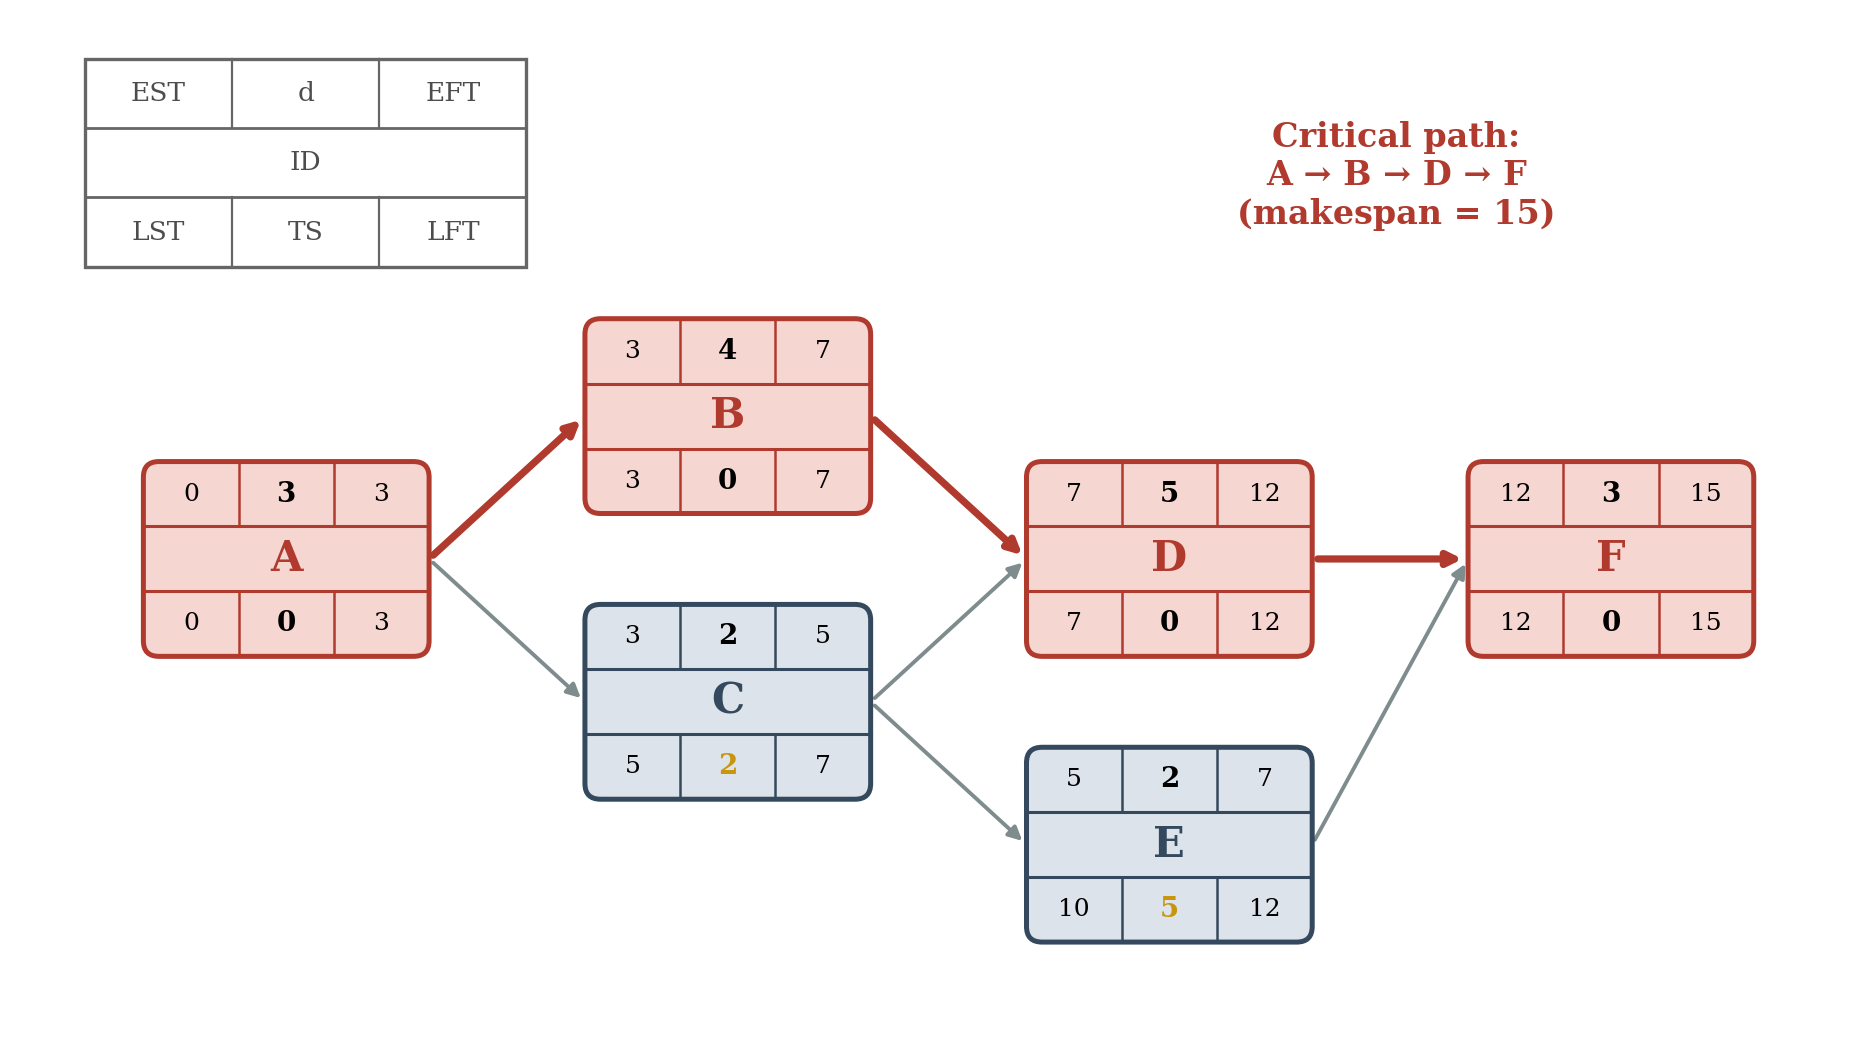
\includegraphics[width=\textwidth]{img/cpm-network.png}
  \caption[CPM activity-on-node network]{Activity-on-node network for the example
  of Table~\ref{tab:example}. Each node shows, from top to bottom,
  $(EST \mid d \mid EFT)$, the activity label, and $(LST \mid TS \mid LFT)$.
  Critical activities ($TS=0$) and the critical path
  $\text{A}\!\rightarrow\!\text{B}\!\rightarrow\!\text{D}\!\rightarrow\!\text{F}$
  are highlighted in red; the makespan is $C_{\max}=15$.}
  \label{fig:cpm-network}
\end{figure}

Applying the forward pass~\eqref{eq:es} and~\eqref{eq:ef} from the start gives
$EST_\text{A}=0,\ EFT_\text{A}=3$; then $EST_\text{B}=EST_\text{C}=EFT_\text{A}=3$, so
$EFT_\text{B}=7$ and $EFT_\text{C}=5$. Activity D waits for both B and C, hence
$EST_\text{D}=\max(EFT_\text{B},EFT_\text{C})=7$ and $EFT_\text{D}=12$. Finally
$EST_\text{F}=\max(EFT_\text{D},EFT_\text{E})=12$ and $EFT_\text{F}=15$, so the
makespan is $C_{\max}=15$.

The backward pass~\eqref{eq:lf} and~\eqref{eq:ls} starts from
$LFT_\text{F}=C_{\max}=15$ and propagates the latest times to the left. The
resulting slacks, from~\eqref{eq:ts}, are
$TS_\text{A}=TS_\text{B}=TS_\text{D}=TS_\text{F}=0$ (critical),
$TS_\text{C}=2$ and $TS_\text{E}=5$. The critical path is thus
$\text{A}\!\rightarrow\!\text{B}\!\rightarrow\!\text{D}\!\rightarrow\!\text{F}$.
Figure~\ref{fig:gantt-slack} renders the same schedule as a Gantt chart, with
each activity at its earliest start and the total float shown as a hatched
reserve to the right of the non-critical activities C and E.

\begin{figure}[htbp]
  \centering
  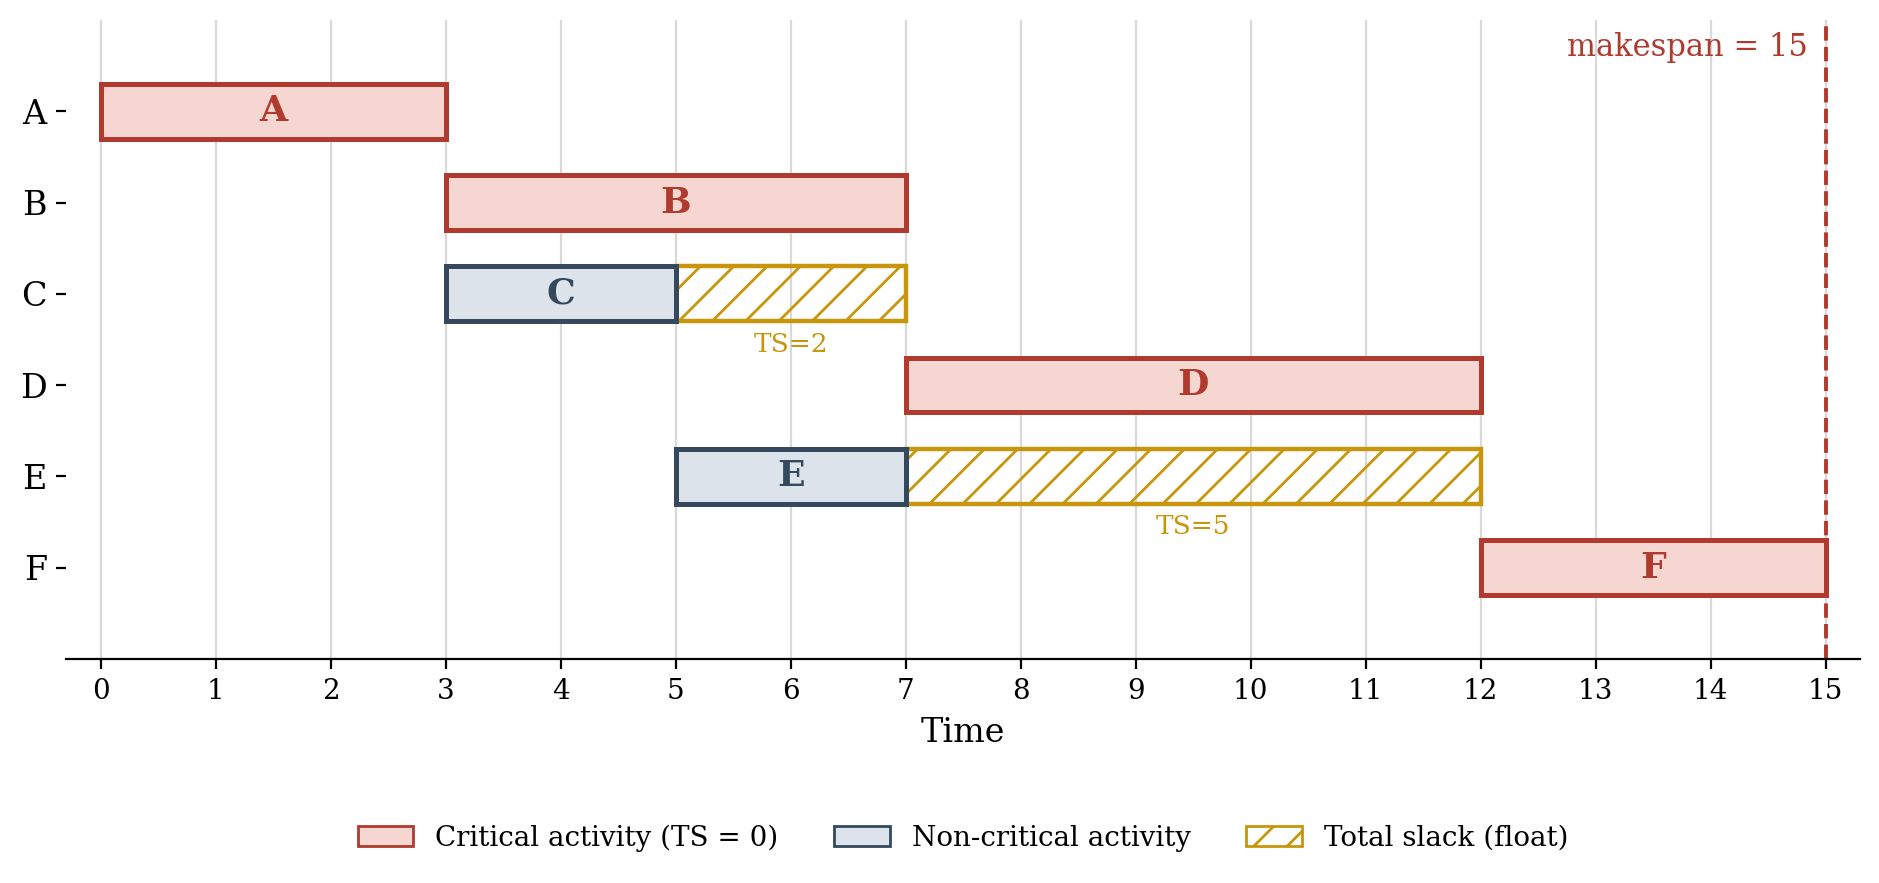
\includegraphics[width=\textwidth]{img/gantt-slack.png}
  \caption[Gantt chart with total float]{Early-start Gantt chart of the example
  project. Solid bars are activities at their earliest start; hatched bars show
  the total float (slack) of the non-critical activities C and E. Critical
  activities have no float and define the makespan $C_{\max}=15$.}
  \label{fig:gantt-slack}
\end{figure}

\subsection{Resource optimisation: levelling and smoothing}
\label{subsec:levelling-smoothing}

CPM as described so far assumes that resources are unlimited. In practice
activities compete for finite resources (people, machines, budget), and a
schedule that is feasible with respect to precedence may over-allocate a
resource~\cite{demeulemeester2002}. \emph{Resource
optimisation} adjusts the start dates of activities so that planned usage never
exceeds availability, and two complementary techniques are
distinguished~\cite{demeulemeester2002}. \emph{Resource levelling} is used when a
shared resource is over-allocated: it may move activities beyond their float,
typically by serialising parallel activities, so the resource limit, not the
precedence logic, drives the schedule. As a result levelling can change the
critical path and usually extends the project
duration~\cite{demeulemeester2002}. \emph{Resource
smoothing}, by contrast, adjusts activities only within their float, so the
critical path and the completion date are preserved while the resource profile
is flattened~\cite{demeulemeester2002}.

The crucial observation for this thesis is that as soon as resources are
limited, the simple longest-path computation of CPM no longer yields a feasible
schedule. Deciding \emph{which} activities to delay, and by how much, in order
to respect resource capacities while keeping the makespan small, is no longer a
polynomial network calculation but a hard combinatorial optimisation problem.
This is precisely the resource-constrained project scheduling problem studied in
the remainder of the thesis.

%==============================================================================
\section{Challenges in project scheduling}
\label{sec:challenges}
%==============================================================================

Adding resource constraints transforms project scheduling into the strongly \emph{NP-hard} Resource-Constrained Project Scheduling Problem (RCPSP)~\cite{blazewicz1983,ganian2020complexity}. The multi-mode extension (MRCPSP) studied here is even harder: once non-renewable resources are present, already \emph{deciding feasibility} (finding any mode assignment that respects the budgets) is NP-complete, as proved by Kolisch and Drexl~\cite{kolischdrexl1994} and confirmed in the recent complexity map of Ganian et al.~\cite{ganian2020complexity}.

This difficulty stems from a massive search space. In the MRCPSP, the exponentially growing combinations of valid start times are further multiplied by the available execution modes~\cite{kolischdrexl1994,hartmann2010survey}. Because exact methods like branch-and-bound can only solve small instances, evolutionary algorithms and other metaheuristics dominate larger applications~\cite{hartmann2002,kolisch2006,khajesaeedi2025review}.

Furthermore, constraints are tightly coupled: resolving a single resource conflict can cascade into new violations or alter the critical path~\cite{demeulemeester2002,khajesaeedi2025review}. Real-world scheduling also introduces conflicting multi-objective goals, such as project lead time versus resource-load balance~\cite{yang2024biobjective} or completion time versus cost~\cite{tian2022multiskill}, and parameter uncertainty~\cite{herroelen2005,ramos2023stochastic}. Standardised evaluation of these complexities relies on established benchmark libraries such as PSPLIB~\cite{kolisch1997} and the larger, multi-mode-specific MMLIB~\cite{vanpeteghem2014}; MMLIB50 and MMLIB100 (Section~\ref{subsec:mmlib}) are what this thesis's own empirical work is evaluated on.

Ultimately, these properties (an exponential, irregular search space, tightly coupled constraints, and the absence of exploitable global structure) make the MRCPSP exceptionally well-suited for population-based metaheuristics. \changed{Evolutionary algorithms require nothing of the problem beyond the ability to evaluate and compare candidate solutions, relying on selection and variation to navigate difficult landscapes. Given their strong empirical record on project scheduling specifically,} from the classic genetic algorithms of Hartmann~\cite{hartmann1998,hartmann2002} to systematic computational comparisons~\cite{kolisch2006,vanpeteghem2014} and recent surveys~\cite{khajesaeedi2025review,dokeroglu2025metaheuristics}, they form the foundation of the approach pursued in the remainder of this thesis.
%==============================================================================
\section{Problem statement and research objectives}
\label{sec:problem-statement}
%==============================================================================
\changed{This section states the target problem precisely
(Section~\ref{subsec:problem-statement}) and derives the research objectives
the thesis pursues (Section~\ref{subsec:objectives}).}
\subsection{Problem statement}
\label{subsec:problem-statement}

This thesis addresses the \emph{Multi-mode Resource-Constrained Project
Scheduling Problem} (MRCPSP)~\cite{brucker1999,hartmann2010survey}. We are given
a project of \emph{non-preemptive} activities \changed{(once started, an activity runs
to completion and cannot be interrupted)}
linked by precedence relations. Each activity may be executed in one of several
\emph{modes}; choosing a mode fixes the duration of the activity and the amounts
of the \emph{renewable} resources (e.g. labour or machines, available afresh each
period) and \emph{non-renewable} resources (e.g. a fixed budget, consumed over
the whole project) that it requires \cite{kolischdrexl1994,hartmann2010survey}.
A solution must select exactly one mode per
activity and a start time for every activity such that

\begin{enumerate}
  \item every activity starts only after all its predecessors have finished
        (precedence feasibility);
  \item at no point in time does the total demand for any renewable resource
        exceed its per-period availability;
  \item the total consumption of each non-renewable resource over the project
        does not exceed its budget.
\end{enumerate}

The objective is to minimise the project \emph{makespan} $C_{\max}$, the
completion time of the final activity, subject to the three constraint classes
above. This is the canonical objective in the benchmark
literature~\cite{kolisch1997,demeulemeester2002}; it reduces to the
single-mode RCPSP when each activity has one mode and to the pure CPM
longest-path problem of Section~\ref{subsec:cpm} when resources are unlimited.
\changed{For the complexity reasons established in Section~\ref{sec:challenges}, this
thesis approaches the problem with an evolutionary
algorithm~\cite{hartmann1998,kolisch2006,vanpeteghem2014,khajesaeedi2025review}.}
As the baseline against which the algorithm proposed in this thesis is compared,
we adopt the genetic-programming hyper-heuristic (GPHH) of
Tian, Mei and Zhang~\cite{Tian2024GPHH}, which learns scheduling rules for the
multi-mode problem and represents a recent, competitive evolutionary approach to
the MRCPSP. The publicly available reference implementation of this GPHH is used
directly as the empirical baseline throughout the experimental evaluation in
Chapter~\ref{chap:experiments}.

\changed{Despite this competitiveness, the baseline leaves several concrete
opportunities unaddressed, in the information it exposes to the evolved
rule, in how it selects parents, and in the absence of any refinement of
the schedules its rules produce. Section~\ref{subsec:research-gap}
substantiates these in full once the necessary formal background is in
place, and Chapter~\ref{chap:approach} targets them with three additive,
independently switchable modifications of the baseline, so that the
individual contribution of each can be isolated experimentally in
Chapter~\ref{chap:experiments}.}

\subsection{Formal definition of the single-mode RCPSP}
\label{subsec:rcpsp-model}

\changed{The informal statement above is now made precise, starting with
the single-mode special case.}
Let $V = \{0, 1, \dots, n, n+1\}$ be the set of activities of a project, where
activity $0$ is a dummy \emph{source} and activity $n+1$ a dummy \emph{sink},
both of zero duration; this is the same activity-on-node convention used
informally in Section~\ref{subsec:cpm}~\cite{demeulemeester2002}, with $n$ the
number of non-dummy activities. Precedence relations form a set of directed
edges $E \subseteq V \times V$, and each activity $j$ has a fixed duration
$d_j \ge 0$ ($d_0 = d_{n+1} = 0$). A set $\mathcal{R}^{\rho}$ of \emph{renewable}
resources is available with a constant per-period capacity $R^{\rho}_k$ for
each $k \in \mathcal{R}^{\rho}$; activity $j$ requires $r^{\rho}_{jk} \ge 0$ units of
resource $k$ for its entire duration. Writing
$A(f,t) = \{\, j \in V : f_j - d_j \le t < f_j \,\}$ for the set of activities
active at time $t$ under a schedule (finish-time vector) $f = (f_j)_{j \in V}$,
the single-mode RCPSP is
\begin{align}
  \text{minimise } \quad & C_{\max} = f_{n+1} \label{eq:rcpsp-obj}\\
  \text{subject to } \quad
  & f_i \le f_j - d_j, && \forall (i,j) \in E, \label{eq:rcpsp-prec}\\
  & \sum_{j \,\in\, A(f,t)} r^{\rho}_{jk} \le R^{\rho}_k, && \forall k \in \mathcal{R}^{\rho},\ \forall t \ge 0, \label{eq:rcpsp-res}\\
  & f_j \ge d_j, && \forall j \in V. \label{eq:rcpsp-nonneg}
\end{align}
Constraint~\eqref{eq:rcpsp-prec} is exactly the precedence relation used by the
forward pass of CPM (Section~\ref{subsec:passes}); constraint~\eqref{eq:rcpsp-res}
is new and couples activities that CPM treats independently. This formulation
follows the conceptual linear-programming model of Demeulemeester and
Herroelen~\cite{demeulemeester2002} for the decision variables $f_j$ and
duration $d_j$, and the resource-classification notation
$\mathcal{R}^\rho,\mathcal{R}^\nu,R^\rho_k$ of Brucker et
al.~\cite{brucker1999}, whose unifying notation for project scheduling this
thesis adopts for resource sets and availabilities throughout.
Without~\eqref{eq:rcpsp-res} the problem reduces to the
longest-path computation of Section~\ref{subsec:cpm}; with it, deciding even
feasibility in the multi-mode case becomes NP-complete, as already noted in
Section~\ref{sec:challenges}.

\subsection{Formal definition of the multi-mode RCPSP}
\label{subsec:mrcpsp-model}

The MRCPSP augments the model of
Section~\ref{subsec:rcpsp-model} with a finite set of execution \emph{modes}
$\mathcal{M}_i$ for every activity $i$ and a second resource class. Choosing mode
$m \in \mathcal{M}_i$ fixes the activity's duration $d_{im}$, its demand $r^{\rho}_{imk}$ for each
renewable resource $k \in \mathcal{R}^{\rho}$, and its consumption $r^{\nu}_{imk}$ of each
\emph{non-renewable} resource $k \in \mathcal{R}^{\nu}$, a resource with a single budget
$R^{\nu}_k$ for the whole project rather than a per-period
capacity~\cite{kolischdrexl1994,hartmann2010survey}. With mode-assignment
variables $m_i \in \mathcal{M}_i$ added to the finish-time variables $f_i$, the model
becomes
\begin{align}
  \text{minimise } \quad & C_{\max} = f_{n+1} \label{eq:mrcpsp-obj}\\
  \text{subject to } \quad
  & f_i \le f_j - d_{j m_j}, && \forall (i,j) \in E, \label{eq:mrcpsp-prec}\\
  & \sum_{j \,\in\, A(f,t)} r^{\rho}_{j m_j k} \le R^{\rho}_k, && \forall k \in \mathcal{R}^{\rho},\ \forall t \ge 0, \label{eq:mrcpsp-res}\\
  & \sum_{j \,\in\, V} r^{\nu}_{j m_j k} \le R^{\nu}_k, && \forall k \in \mathcal{R}^{\nu}, \label{eq:mrcpsp-nr}\\
  & m_j \in \mathcal{M}_j,\ f_j \ge d_{j m_j}, && \forall j \in V. \label{eq:mrcpsp-mode}
\end{align}
Constraint~\eqref{eq:mrcpsp-nr} is what distinguishes the MRCPSP from a simple
RCPSP with per-mode durations: because it sums over the \emph{entire} project
rather than over a time window, it can be \changed{checked} only after every mode has
been fixed, which is exactly why Kolisch and Drexl proved that even checking
feasibility of a mode assignment is NP-complete~\cite{kolischdrexl1994}.
Setting $|\mathcal{M}_i|=1$ for every activity recovers the single-mode
model~\eqref{eq:rcpsp-obj}--\eqref{eq:rcpsp-nonneg} exactly.
Early heuristics for this exact problem combined a hand-designed priority rule
for activity selection with a second, equally hand-designed rule for mode
selection~\cite{boctor1996new,kolisch1994priority,lova2006mrcpsp}.

\subsection{A taxonomy of realistic extensions}
\label{subsec:taxonomy}

The MRCPSP is itself one of several directions in which the basic RCPSP has been
extended to better match real projects~\cite{hartmann2010survey,mika2015mrcpsp}.
Figure~\ref{fig:rcpsp-taxonomy} situates it among the variants most discussed
in the recent literature:
\begin{description}
  \item[Generalized precedence relations (MRCPSP/max)] replace the simple
        finish-to-start relation of~\eqref{eq:mrcpsp-prec} with minimal and
        maximal time lags between any pair of activities, first formalised by
        Bartusch, M\"ohring and Radermacher~\cite{bartusch1988}; even feasibility
        is NP-hard under this extension~\cite{hartmann2010survey}.
  \item[Preemptive variants] allow an activity to be interrupted and resumed
        later, trading schedule flexibility for a more complex SGS that must
        track partially completed activities~\cite{vanpeteghem2010}.
  \item[Multi-skill RCPSP] replaces anonymous renewable resources with named
        workers who each master a subset of required skills, adding a
        many-to-one assignment problem on top of scheduling; Tian et
        al.~\cite{tian2022multiskill} formulate this jointly with mode and
        skill-switch decisions for the multi-objective case.
  \item[Stochastic and robust RCPSP] treat durations or resource availability as
        uncertain rather than fixed, an issue surveyed early by Herroelen and
        Leus~\cite{herroelen2005} and addressed for the multi-mode case by Ramos
        et al.~\cite{ramos2023stochastic} with a multi-start iterated local
        search over a stochastic-programming formulation.
  \item[Multi-objective RCPSP] optimises makespan jointly with a second
        criterion, e.g. cost or resource-load balance; Yang et
        al.~\cite{yang2024biobjective} combine NSGA-II with $Q$-learning for a
        bi-objective (lead time vs.\ resource-load balance) multi-mode
        multi-project variant.
  \item[Dynamic / disrupted RCPSP] reacts online to disruptions revealed during
        execution, e.g. resource breakdowns, rather than planning the whole
        project up front~\cite{cai2024rlgnn}; Ruhlusara\c{c} and \c{C}al{\i}\c{s}kan
        address the related dynamic multi-mode \emph{multi-project} setting with
        an MILP model minimising weighted earliness and tardiness, validated on
        a real furniture-manufacturing case~\cite{ruhlusarac2022dynamic}.
\end{description}

\begin{figure}[htbp]
  \centering
  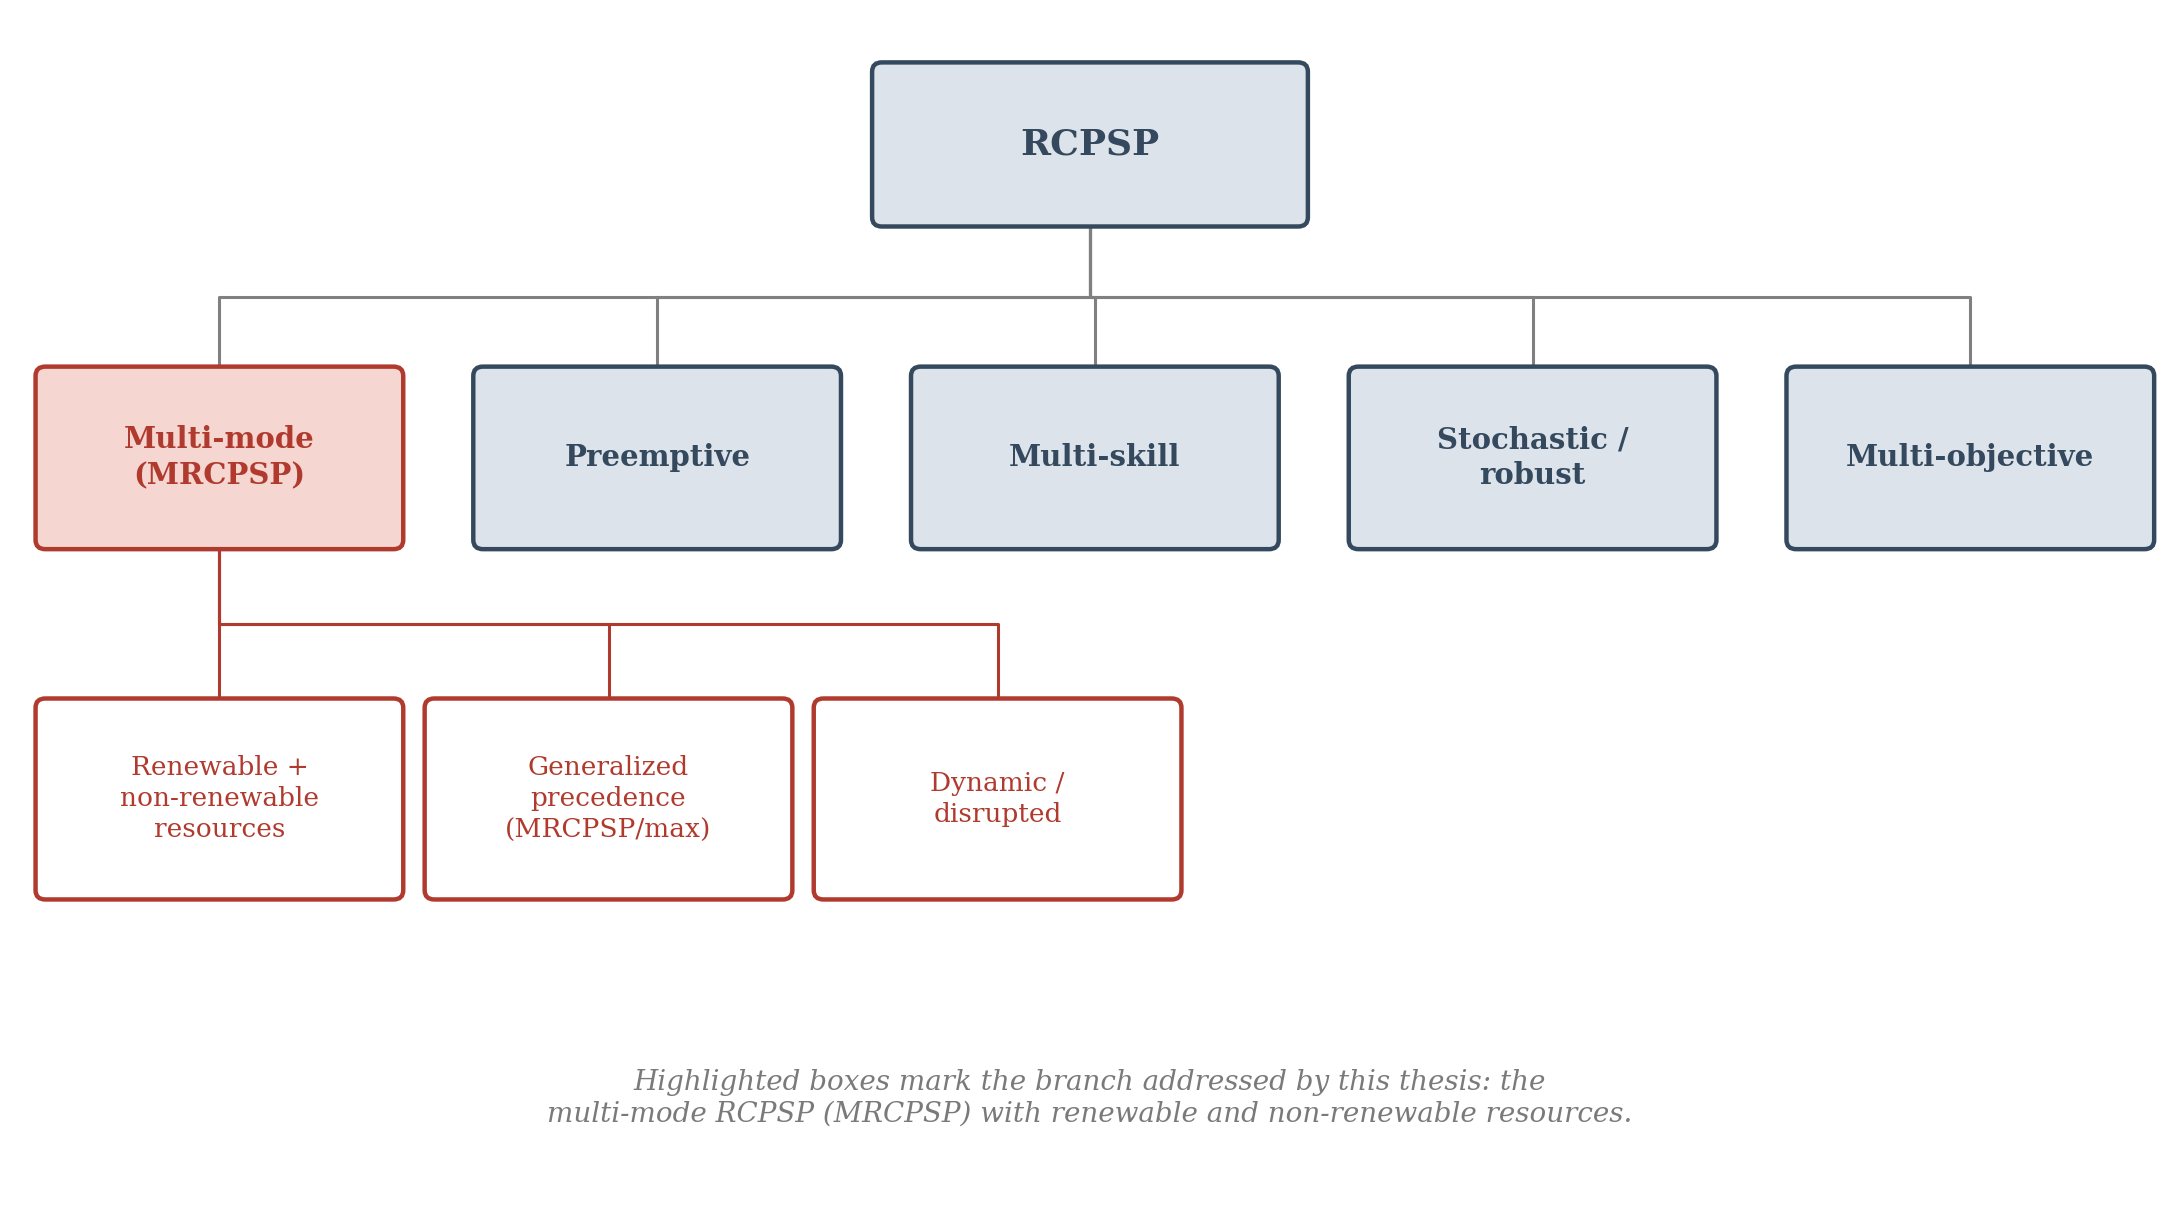
\includegraphics[width=0.92\textwidth]{img/rcpsp-taxonomy.png}
  \caption[Taxonomy of RCPSP extensions]{A taxonomy of realistic RCPSP
  extensions. This thesis addresses the multi-mode branch (MRCPSP) with both
  renewable and non-renewable resources (highlighted), the variant formalised
  in Section~\ref{subsec:mrcpsp-model}.}
  \label{fig:rcpsp-taxonomy}
\end{figure}

These extensions are not mutually exclusive (the multi-skill and
multi-objective variants above are themselves built on top of the multi-mode
model), which is why Hartmann and Briskorn's survey organises them as a
combinable feature set rather than a strict
hierarchy~\cite{hartmann2010survey}. Structural extensions beyond this
taxonomy also exist: van der Beek et al.~\cite{VanDerBeek2024} keep a single
makespan objective but relax which activities must even be executed (a
\emph{flexible project structure} in which only a subset of each ``selection
group'' need run) and allow non-renewable resources to be both consumed and
produced over the project, solving the resulting problem with a hybrid
differential-evolution algorithm, illustrating that real projects can
violate assumptions, such as a fixed activity set, that every variant above
still takes for granted. The present thesis keeps to the
``plain'' renewable-and-non-renewable MRCPSP of
Section~\ref{subsec:mrcpsp-model}, the variant for which the standard MMLIB and
PSPLIB benchmarks (Chapter~\ref{chap:dataset}) and the baseline algorithm of
Section~\ref{subsec:problem-statement} are defined.

\subsection{Research objectives}
\label{subsec:objectives}

The thesis pursues the following objectives:

\begin{enumerate}
  \item \textbf{Design.} To design a custom evolutionary algorithm for the
        MRCPSP.
  \item \textbf{Implementation.} To implement the algorithm in Python in a way
        that is reproducible and that can read the standard PSPLIB and MMLIB
        instance formats.
  \item \textbf{Analysis.} To analyse the behaviour of the algorithm 
        in order to understand which design choices
        contribute most to its performance.
  \item \textbf{Evaluation.} To evaluate the algorithm on the MMLIB50 and
        MMLIB100 benchmark sets~\cite{vanpeteghem2014} using standard
        quality metrics, and to compare it against our baseline, the
        genetic-programming hyper-heuristic of Tian, Mei and
        Zhang \cite{Tian2024GPHH}.
  \item \textbf{Discussion.} To discuss the computational complexity,
        scalability and limitations of the proposed approach, and to identify
        directions for future work.
\end{enumerate}

\chapter{Overview of current approaches}
\label{chap:overview}

\changed{This chapter surveys how the (M)RCPSP is solved in the literature
and identifies the gap the proposed algorithm addresses. It first
introduces the schedule generation schemes and the solution representation
that virtually every heuristic for the problem shares
(Section~\ref{sec:rcpsp-formalization}), then evolutionary algorithms and
genetic programming (Section~\ref{sec:ea-metaheuristics}), and finally the
existing exact and metaheuristic approaches together with the research gap
(Section~\ref{sec:existing-approaches}).}

%==============================================================================
\section{\texorpdfstring{\changed{Schedule generation schemes and solution representation}}{Schedule generation schemes and solution representation}}
\label{sec:rcpsp-formalization}
%==============================================================================

\changed{This section introduces the schedule generation scheme used by
almost every (M)RCPSP heuristic to decode priorities into feasible
schedules, and connects it to solution representation, continuing the
worked example of Table~\ref{tab:example} under an added resource
constraint.}

\subsection{Schedule generation schemes}
\label{subsec:sgs}

Constraint~\eqref{eq:rcpsp-res} cannot be resolved by a single forward pass: at
any point several activities may be precedence-eligible while only some of them
fit within the remaining resource capacity. Almost every constructive heuristic
and every metaheuristic for the RCPSP therefore builds a schedule with a
\emph{schedule generation scheme} (SGS), a step-wise procedure that, at each
step, chooses one eligible activity from a \emph{decision set} and fixes its
start time so that~\eqref{eq:rcpsp-res} stays satisfied, until every activity is
scheduled~\cite{kolisch1996sgs}. The two classical variants differ in their
decision set:
\begin{description}
  \item[Serial SGS] processes activities one at a time. At each step the decision
        set $D$ contains every unscheduled activity whose predecessors are
        already scheduled; one activity is selected from $D$ (by a priority
        rule, see below) and given the earliest start time that respects both
        precedence and the resource capacities given everything scheduled so
        far. Serial SGS always reaches a so-called \emph{active} schedule:
        \changed{one in which no activity can be started earlier without delaying
        some other activity or violating a constraint. This matters because
        the set of active schedules is guaranteed to contain an optimal
        solution, so restricting the search to them loses
        nothing~\cite{kolisch1996sgs}.}
  \item[Parallel SGS] advances a clock $t$ instead of an activity counter. At
        each decision point $t$ it forms the set of all activities that are
        precedence-eligible \emph{and} resource-feasible at $t$, schedules as
        many of them as the remaining capacity allows (again by priority), and
        then advances $t$ to the next finish time.
\end{description}
Kolisch's empirical comparison of the two schemes is more nuanced than the
active-schedule argument alone suggests: in single-pass mode parallel SGS
actually attains a \emph{lower} average deviation from the optimum than
serial SGS, and under biased random sampling serial SGS only pulls ahead for
larger sample sizes and moderately resource-constrained instances, with
parallel SGS remaining competitive for small samples and tightly constrained
instances~\cite{kolisch1996sgs}. This thesis nonetheless adopts serial SGS as
the default decoding procedure throughout, since it alone is guaranteed to
reach the active-schedule space containing the optimum (the argument above),
with the parallel variant reserved for the dual-decoding experiments of
Chapter~\ref{chap:approach}. \changedB{Algorithms~\ref{alg:parallel-sgs}
and~\ref{alg:serial-sgs} state the two variants in full, each driven by a
generic priority rule $\pi$; Chapter~\ref{chap:approach} instantiates the
serial variant with the evolved rule pair that drives it in this thesis.}

\begin{algorithm}[htbp]
\caption[Parallel SGS with a priority rule]{\changed{Parallel SGS with a
priority rule $\pi$ (lower value = higher priority).}}
\label{alg:parallel-sgs}
\begin{algorithmic}[1]
\Require instance with activities $V$; priority rule $\pi$
\State $t \gets 0$;\quad $S \gets \emptyset$ \Comment{clock and scheduled set}
\While{$S \neq V$}
  \State $D_t \gets \{\, j \in V \setminus S : \text{all predecessors of } j$
    \Statex \hspace{\algorithmicindent}\hspace{\algorithmicindent}
    $\text{finished by } t \text{ and } j \text{ resource-feasible at } t \,\}$
  \While{$D_t \neq \emptyset$}
    \State $j^{*} \gets \arg\min_{j \in D_t} \pi(j)$; start $j^{*}$ at time $t$;
      $S \gets S \cup \{j^{*}\}$
    \State recompute $D_t$ under the reduced remaining capacity at $t$
  \EndWhile
  \State $t \gets$ the earliest finish time of a running activity after $t$
\EndWhile
\State \Return the completed schedule
\end{algorithmic}
\end{algorithm}

\begin{algorithm}[htbp]
\caption[Serial SGS with a priority rule]{\changedB{Serial SGS with a
priority rule $\pi$ (lower value = higher priority).}}
\label{alg:serial-sgs}
\begin{algorithmic}[1]
\Require instance with activities $V$; priority rule $\pi$
\State $S \gets \emptyset$ \Comment{already-scheduled activities}
\While{$S \neq V$}
  \State $D \gets \{\, j \in V \setminus S : \text{all predecessors of } j \text{ are in } S \,\}$ \Comment{decision set}
  \State $j^{*} \gets \arg\min_{j \in D} \pi(j)$
  \State start $j^{*}$ at the earliest time respecting precedence and
    resource capacities
  \State update remaining resource availabilities; $S \gets S \cup \{j^{*}\}$
\EndWhile
\State \Return the completed schedule
\end{algorithmic}
\end{algorithm}

\subsection{Solution representation: from chromosomes to schedules}
\label{subsec:representation-intro}

An SGS by itself only decides feasibility; it needs a \emph{priority value} for
every activity in the decision set to break ties between simultaneously
eligible activities. The classical representation, going back to the first
genetic algorithms for the RCPSP~\cite{hartmann1998}, encodes a solution as an
\emph{activity list}: a permutation of $V$ that respects all precedence
relations (a topological order of the activity network). Decoding such a
chromosome with one pass of the serial SGS (always select, from the current
decision set, the eligible activity that appears earliest in the list) yields
exactly one feasible schedule for exactly one problem instance. This
representation-then-decoding split, chromosome on one side and SGS on the
other, is what later allows genetic \emph{programming} to replace the
chromosome with a reusable priority \emph{rule}, as
Section~\ref{sec:ea-metaheuristics} develops.

\subsubsection*{Worked example, continued}

Table~\ref{tab:example} introduced six activities with no resource constraints;
Figure~\ref{fig:cpm-network} found a makespan of 15. Suppose now a single
renewable resource $R$ of capacity 2 is added, with per-activity demands
$r_A=1,\, r_B=2,\, r_C=1,\, r_D=2,\, r_E=1,\, r_F=1$. The unconstrained schedule
of Figure~\ref{fig:gantt-slack} is no longer resource-feasible, since it runs
$B$ and $C$ concurrently from $t=3$ to $t=5$, a combined demand of $1+2=3 > 2$.
Decoding the activity-list chromosome $[A, C, E, B, D, F]$ with the serial SGS of
Section~\ref{subsec:sgs} resolves the conflict: $A$ and $C$ are scheduled as
before, but $B$, although precedence-eligible from $t=3$, right after $A$
finishes, cannot start until $t=7$, because at any earlier time its demand of
2 units would push the combined usage with the still-active $C$ or $E$ above
the capacity of 2. Only once $C$ and $E$ have both finished does enough capacity
free up. Activities $D$ and $F$ then simply follow in precedence order, giving
the schedule and Gantt chart of Figure~\ref{fig:sgs-decoding} and a makespan of
19: four time units above the unconstrained CPM value, a gap attributable
entirely to resource contention rather than precedence.

\begin{figure}[htbp]
  \centering
  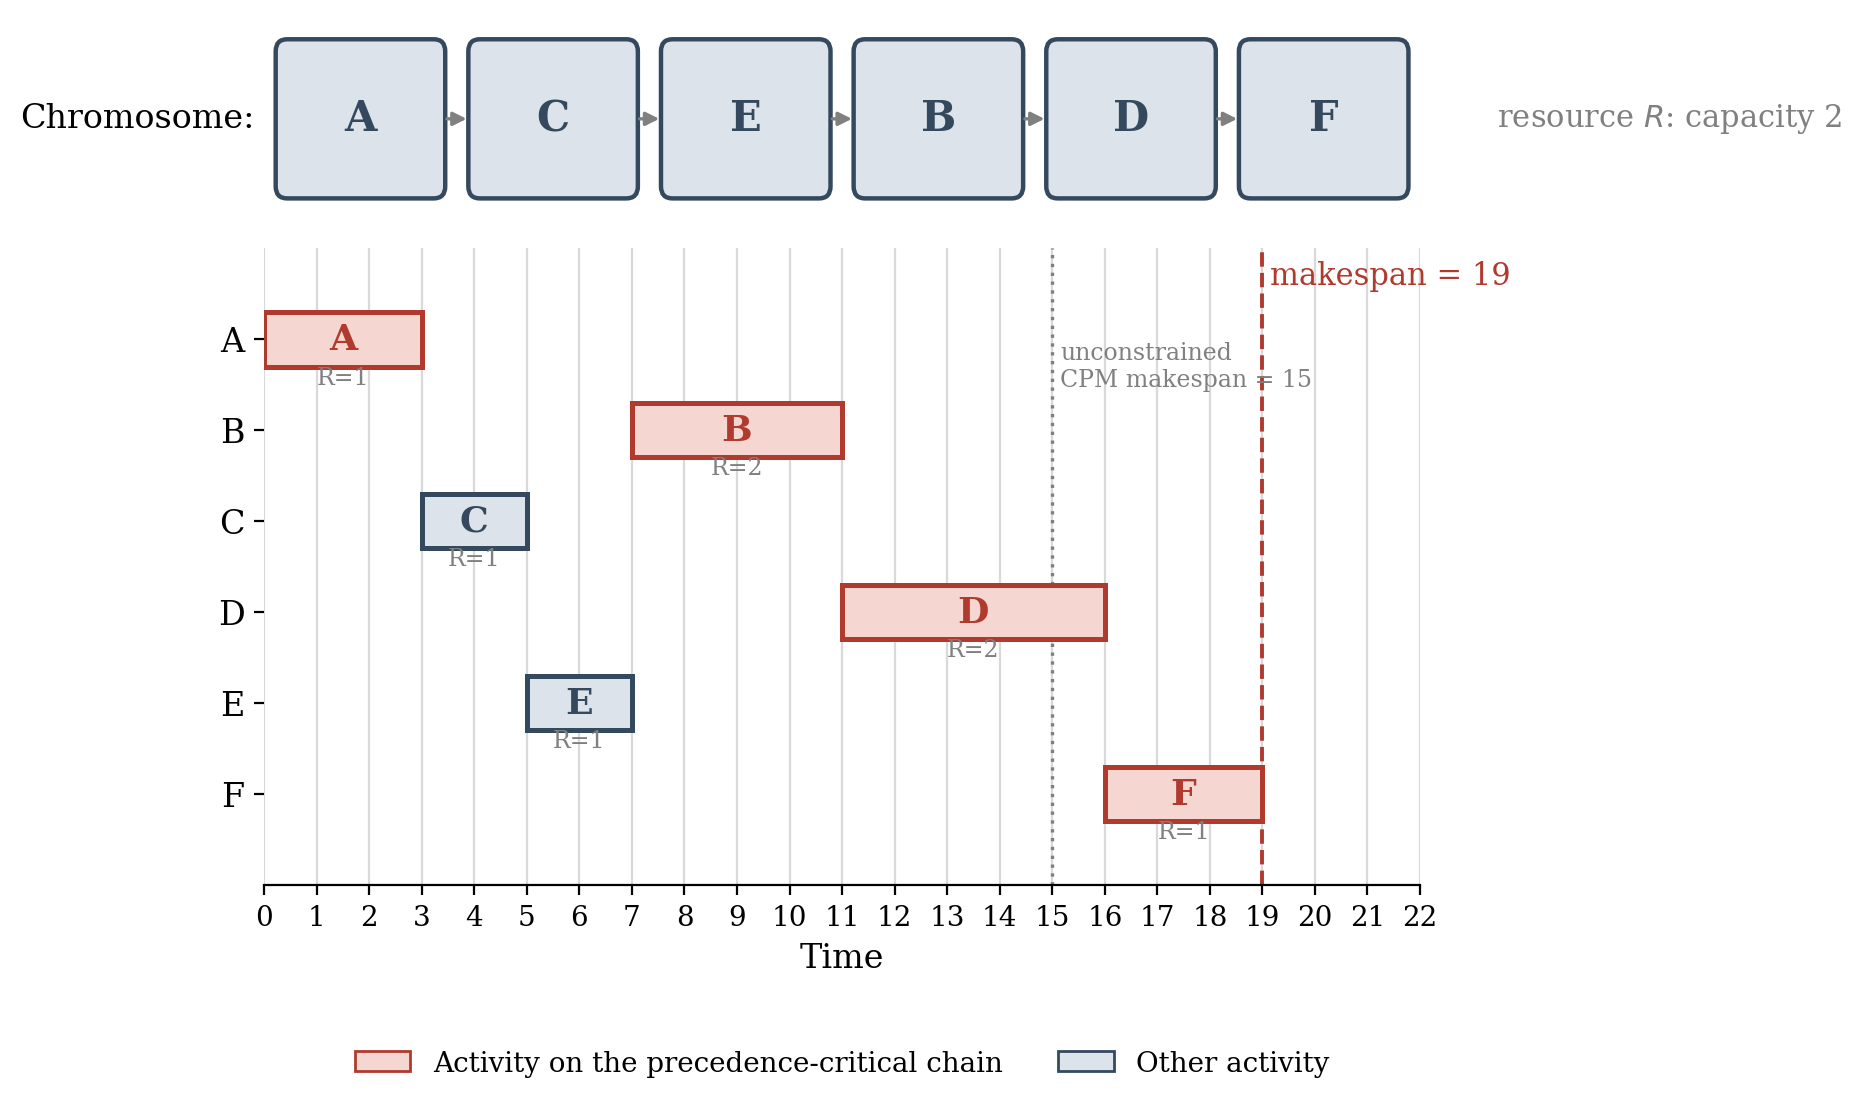
\includegraphics[width=\textwidth]{img/sgs-decoding.png}
  \caption[Serial SGS decoding under a resource constraint]{Decoding the
  activity-list chromosome $[A,C,E,B,D,F]$ with the serial SGS, under a single
  renewable resource $R$ of capacity 2 (demands shown below each bar). Activity
  $B$ is delayed from its precedence-eligible time $t=3$ to $t=7$ by resource
  contention with $C$ and $E$; the resulting makespan is 19, against the
  unconstrained CPM value of 15 (Figure~\ref{fig:gantt-slack}).}
  \label{fig:sgs-decoding}
\end{figure}

%==============================================================================
\section{Evolutionary algorithms and metaheuristics}
\label{sec:ea-metaheuristics}
%==============================================================================

\changed{This section introduces the algorithmic family on which the rest of the
thesis builds: the evolutionary loop shared by every such algorithm, and
the two representations relevant here, the fixed-length chromosome of a
genetic algorithm and the variable-size program tree of genetic
programming.}

\subsection{The general evolutionary loop}
\label{subsec:ea-loop}

An evolutionary algorithm (EA) maintains a \emph{population} of candidate
solutions, called individuals, and repeatedly applies three biologically
inspired operators to it: \emph{selection} favours individuals with better
fitness as parents; \emph{variation} (crossover and mutation) produces offspring
by recombining or perturbing parents; and \emph{replacement} forms the next
generation from parents and offspring, usually again biased toward
fitness. No assumption is made about the objective being
convex, differentiable, or even computable in closed form, only that
candidate solutions can be evaluated and compared, which is precisely why EAs
remain effective on a combinatorially structured, discontinuous landscape such
as the RCPSP makespan surface described in
Section~\ref{sec:challenges}~\cite{dokeroglu2025metaheuristics}.
Figure~\ref{fig:ea-loop} depicts this cycle.
What changes between EA \emph{families} is the representation of an
individual and the variation operators defined on it; the next two subsections
contrast the two representations relevant to this thesis.

\begin{figure}[htbp]
  \centering
  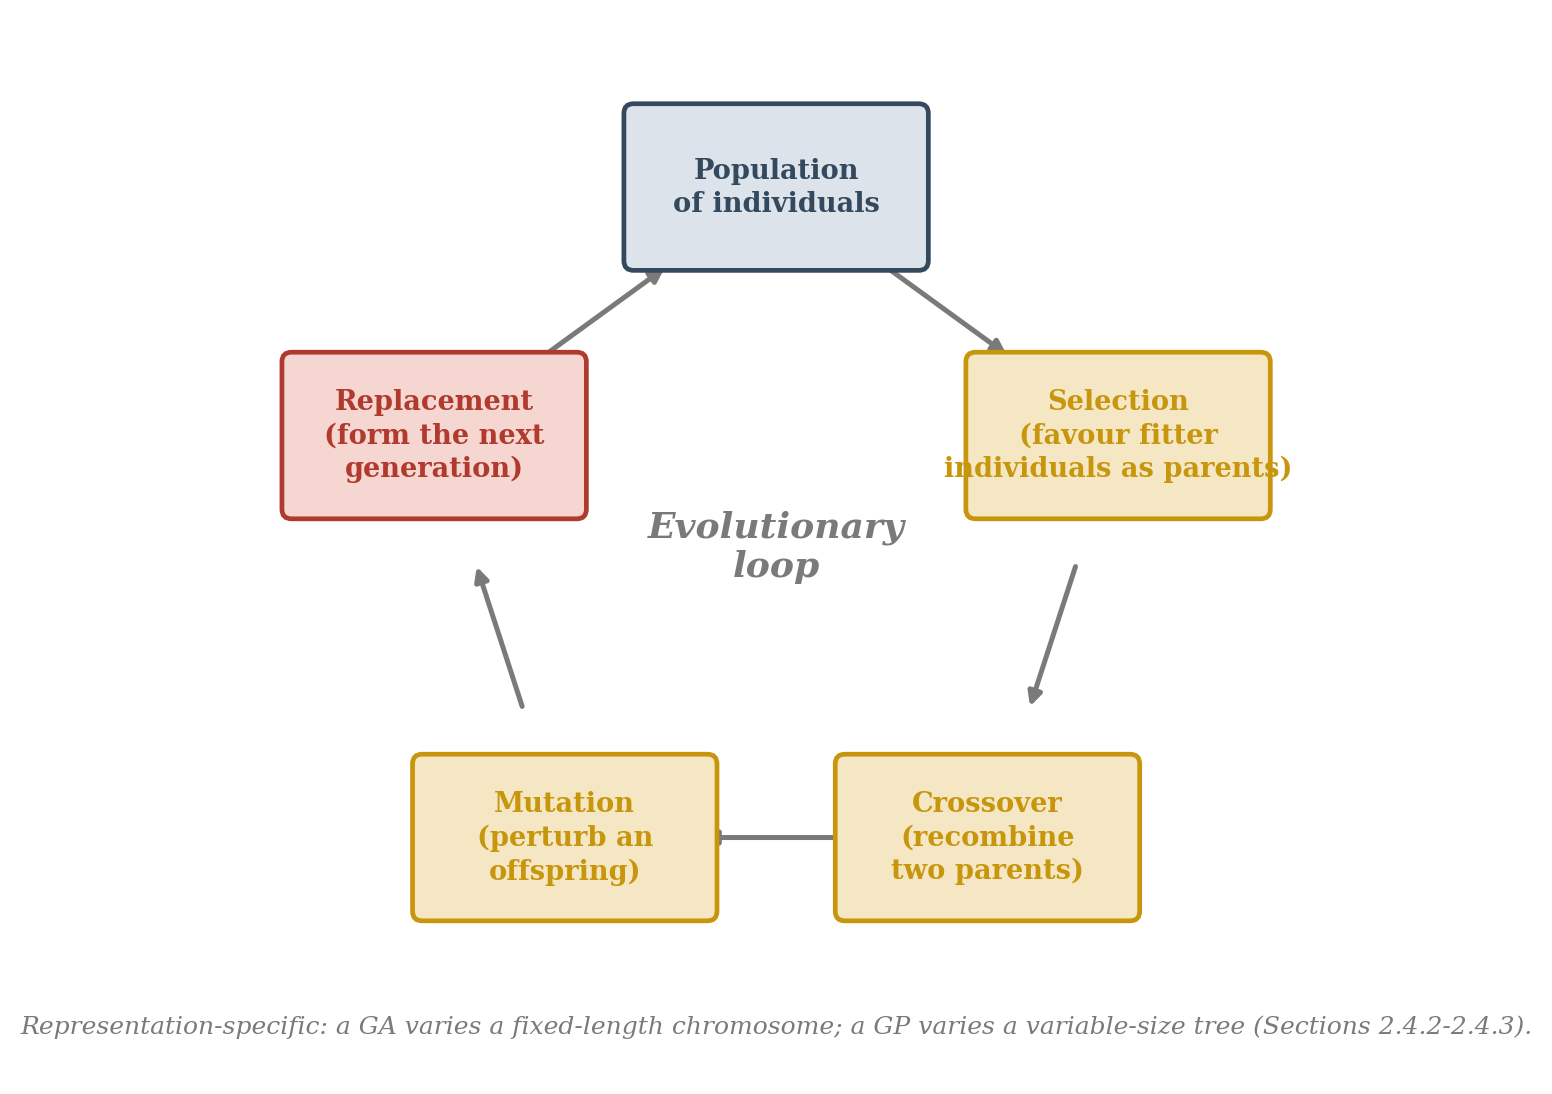
\includegraphics[width=0.72\textwidth]{img/ea-loop.png}
  \caption[The general evolutionary loop]{The general evolutionary loop
  shared by every EA family discussed in this thesis: selection biases which
  individuals become parents, crossover and mutation jointly form the
  variation step that produces offspring, and replacement assembles the next
  generation. Sections~\ref{subsec:ga-rcpsp} and~\ref{subsec:gp-hh} keep this
  loop fixed and contrast only the representation on which crossover and
  mutation operate.}
  \label{fig:ea-loop}
\end{figure}

\subsection{Genetic algorithms for (M)RCPSP}
\label{subsec:ga-rcpsp}

A genetic algorithm (GA) represents each individual as a fixed-length
chromosome over a finite alphabet, classically a bit string, and applies
generic operators such as one-point crossover or bit-flip mutation defined
purely on that encoding. Applied to the RCPSP, the
chromosome is the activity-list permutation of
Section~\ref{subsec:representation-intro}, possibly paired with a
mode-assignment list for the multi-mode case; specialised operators such as
precedence-preserving crossover keep every offspring chromosome a valid
topological order~\cite{hartmann1998,hartmann2002}. Decoding with the serial SGS
of Section~\ref{subsec:sgs} converts the chromosome into a fitness value (the
makespan); Van Peteghem and Vanhoucke's GA for the preemptive and
non-preemptive MRCPSP, and its extension to a wide instance set, established
this activity-list-plus-SGS design as the standard GA baseline for the multi-mode
problem~\cite{vanpeteghem2010,vanpeteghem2014}. Crucially, the chromosome
\emph{is} the schedule of one specific instance: evolving a population means
searching for one good solution, and the search must restart from scratch for
every new project.

\subsection{Genetic programming and hyper-heuristics}
\label{subsec:gp-hh}

Genetic programming (GP), introduced by Koza as a way of \changedB{evolving} computer
programs rather than fixed-length strings~\cite{koza1994gp}, keeps the
evolutionary loop of
Section~\ref{subsec:ea-loop} but replaces the fixed-length chromosome with a
variable-size syntax tree, typically representing an arithmetic or logical
expression: internal nodes are \emph{functions} (e.g. $+, -, \min$) and leaves
are \emph{terminals} (input features or constants).
Subtree crossover exchanges randomly chosen subtrees between two parent trees,
and subtree mutation replaces a subtree with a freshly generated random one;
because every well-formed subtree is itself a well-formed tree, these operators
need no special repair mechanism to stay closed under the representation.

When a GP tree is interpreted not as a direct solution but as a \emph{priority
rule} (compiled once and then queried by an SGS every time it must break a tie
in the decision set), the result is a \emph{genetic-programming
hyper-heuristic} (GPHH): instead of searching for one schedule, the algorithm
searches for one re-usable rule that an SGS can apply to \emph{any} instance of
the problem class~\cite{branke2016gphh}.
Figure~\ref{fig:representation-contrast} contrasts the two representations
directly: the GA chromosome of Section~\ref{subsec:ga-rcpsp} decodes, with one
SGS pass, into a single schedule for a single instance, whereas a GP tree such
as $\min(\mathrm{LST},\, \mathrm{GRPW} - \mathrm{Duration})$ is compiled into a
priority function that an SGS can query on an unseen instance without any
further evolution. This shift from instance-specific solutions to
generalisable rules is what makes GPHH attractive whenever many related
instances must be solved repeatedly, exactly the setting evaluated in
Chapter~\ref{chap:experiments}, and it is the representation adopted by the
baseline of this thesis~\cite{Tian2024GPHH}.

\begin{figure}[htbp]
  \centering
  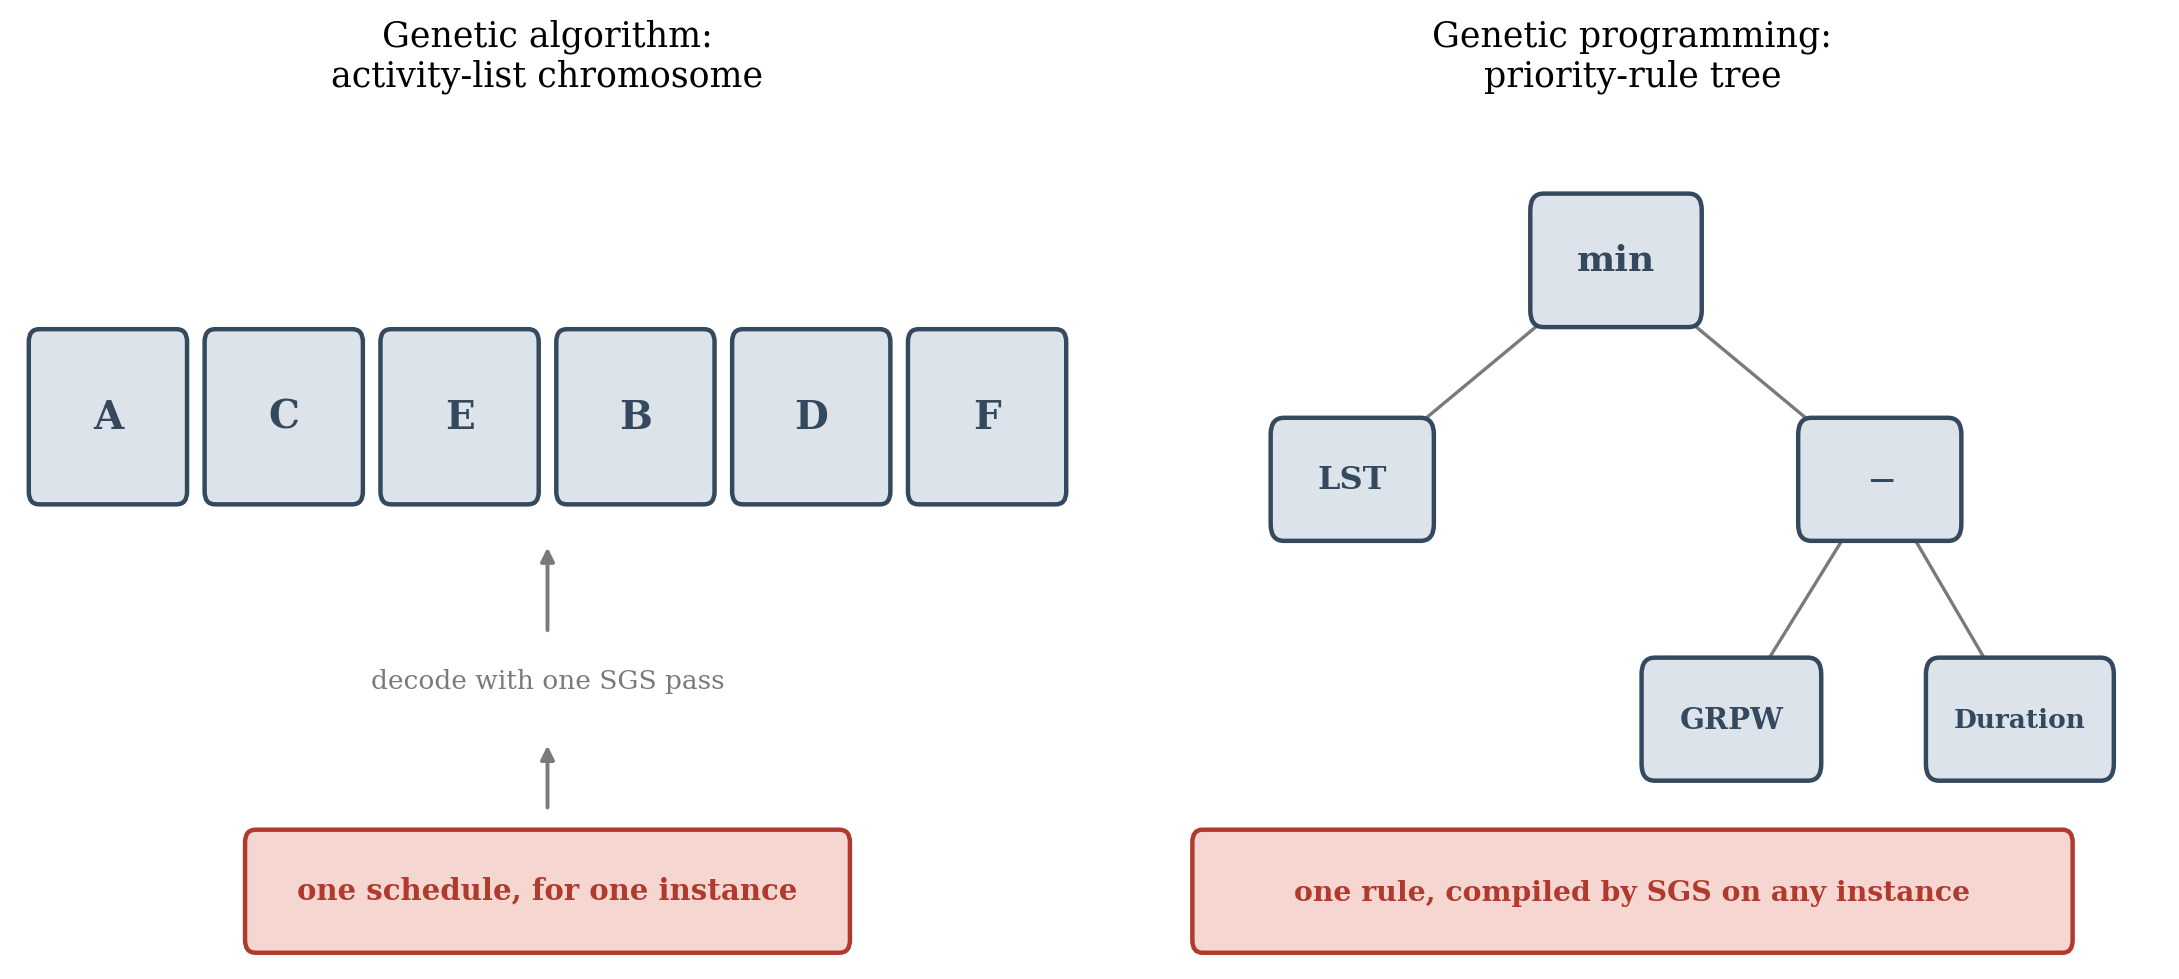
\includegraphics[width=0.92\textwidth]{img/representation-contrast.png}
  \caption[GA chromosome vs.\ GP priority-rule tree]{The representation
  contrast between a genetic algorithm and a genetic-programming
  hyper-heuristic. The GA chromosome decodes, via one SGS pass, into a schedule
  for one instance; the GP tree is a priority rule that an SGS can compile and
  apply to any instance of the problem class.}
  \label{fig:representation-contrast}
\end{figure}

%==============================================================================
\section{Existing approaches for (M)RCPSP}
\label{sec:existing-approaches}
%==============================================================================

\changed{This section surveys how the literature has actually solved the (M)RCPSP,
moving from exact methods through metaheuristics and local search to the
genetic-programming hyper-heuristics most directly related to this thesis,
and closes with the specific gap that Chapter~\ref{chap:approach}
addresses.}

\subsection{Exact methods}
\label{subsec:exact}

Exact algorithms for the MRCPSP are almost exclusively branch-and-bound
procedures that explore the space of precedence- and resource-feasible partial
schedules, pruned with lower bounds derived from the (mode-relaxed) critical
path; this style of bounding remains the reference point for newer exact
formulations, e.g. for the generalized-precedence
MRCPSP/max~\cite{bartusch1988}. Because the underlying decision problem is
NP-complete (Section~\ref{subsec:mrcpsp-model}), these methods scale to at most
a few dozen activities before running times become impractical, which is the
chief reason that metaheuristics dominate the literature for realistically sized
instances~\cite{demeulemeester2002,hartmann2010survey}. Recent work narrows
this gap from two directions rather than closing it outright: Chakrabortty,
Sarker and Essam reduce the variable count of event-based \changed{mixed-integer
linear programming (MILP)} formulations
for the MRCPSP~\cite{chakrabortty2014event}, while Vanhoucke and Coelho
combine branch-and-bound with metaheuristic-style restriction of the search
space in a matheuristic that reports new best-known solutions on standard
RCPSP benchmarks~\cite{vanhoucke2024matheuristic}, building on their earlier
result that the feasible solution space of an RCPSP instance can itself be
reduced without excluding any optimum~\cite{vanhoucke2024reducing}. Neither
line of work scales to the MMLIB50/MMLIB100 instance sizes used in this
thesis (Chapter~\ref{chap:dataset}).

\subsection{Classical and recent metaheuristics}
\label{subsec:metaheuristics}

Besides the genetic algorithms already discussed in
Section~\ref{subsec:ga-rcpsp}, the RCPSP and MRCPSP have been attacked with
essentially every major metaheuristic framework: simulated annealing, tabu
search, scatter search, ant colony optimisation and particle swarm
optimisation, each paired with the activity-list-plus-SGS encoding of
Section~\ref{subsec:representation-intro} and a framework-specific notion of
neighbourhood or pheromone update~\cite{kolisch2006,khajesaeedi2025review}.
Table~\ref{tab:recent-approaches} samples how active this line of work remains:
Peng et al.~\cite{peng2023quantumpso}
hybridise quantum-behaved particle swarm optimisation with the JAYA search
operator for a multi-skill multi-mode variant; and Cai, Bian and
Liu~\cite{cai2024rlgnn} depart from population-based search altogether, training
a graph-neural-network policy with proximal policy optimisation to schedule
under resource disruptions. Mirror-based and hybrid differential-evolution
GAs continue to be proposed for the plain MRCPSP itself: Zamani's mirror GA
solves an instance and a mode-inverted counterpart in parallel and reports
results competitive with or better than earlier GA baselines on PSPLIB and
MMLIB~\cite{zamani2019mirror}, and Cheng and Tran combine chaotic search with
fuzzy $c$-means clustering in a differential-evolution algorithm specifically
to avoid the premature convergence that plagues simpler
GAs~\cite{cheng2016fcde}. Priority-rule design itself also remains an active
topic in its own right: Buddhakulsomsiri and Kim extend priority-rule
heuristics with resource vacations and activity
splitting~\cite{buddhakulsomsiri2007}, and Adamu, Okagbue and Oguntunde
combine several classical rules into a single hybrid rule via machine
learning~\cite{adamu2019priority}, both hand-designing exactly the kind of
composite priority function that the GP of Chapter~\ref{chap:approach}
instead evolves automatically. Across this diversity, the encoding and decoding
machinery of Sections~\ref{subsec:representation-intro}
and~\ref{subsec:ga-rcpsp} is shared almost universally; what differs is how
candidate priority lists are proposed and accepted.

\begin{table}[htbp]
  \centering
  \caption[Representative metaheuristic approaches for (M)RCPSP]{\changed{Representative
  metaheuristic approaches for (M)RCPSP, in
  chronological order, illustrating the range of frameworks (swarm,
  local-search, learning-based and evolutionary) applied to the problem.}}
  \label{tab:recent-approaches}
  \begin{tabularx}{\textwidth}{@{}>{\raggedright\arraybackslash}X >{\raggedright\arraybackslash}p{3.1cm} >{\raggedright\arraybackslash}X c@{}}
    \toprule
    \textbf{Method} & \textbf{Reference} & \textbf{Problem variant} & \textbf{Year} \\
    \midrule
    Fuzzy-clustering chaotic DE & Cheng and Tran~\cite{cheng2016fcde} & Multi-mode & 2016 \\
    Mirror-based GA & Zamani~\cite{zamani2019mirror} & Multi-mode & 2019 \\
    MILP, weighted earliness/tardiness & Ruhlusara\c{c} and \c{C}al{\i}\c{s}kan~\cite{ruhlusarac2022dynamic} & Dynamic, multi-mode, multi-project & 2022 \\
    Hybrid quantum PSO & Peng et al.~\cite{peng2023quantumpso} & Multi-skill, multi-mode & 2023 \\
    Multi-start iterated local search & Ramos et al.~\cite{ramos2023stochastic} & Stochastic, multi-mode & 2023 \\
    RL with graph neural network & Cai et al.~\cite{cai2024rlgnn} & Resource disruptions & 2024 \\
    NSGA-II + $Q$-learning & Yang et al.~\cite{yang2024biobjective} & Multi-objective, multi-project & 2024 \\
    Hybrid differential evolution & van der Beek et al.~\cite{VanDerBeek2024} & Flexible project structure & 2024 \\
    Two-tree GPHH (this thesis' baseline) & Tian et al.~\cite{Tian2024GPHH} & Multi-mode & 2024 \\
    Multi-tree GP, knee-point grouping & Tian et al.~\cite{tian2025multitree} & Dynamic, multi-mode & 2025 \\
    \bottomrule
  \end{tabularx}
\end{table}

\subsection{Local search and schedule improvement}
\label{subsec:local-search}

Orthogonal to how a priority list is searched is how the schedule it decodes
into can be \emph{improved after the fact}, without changing the underlying
list. The best-known such technique is \emph{justification}: starting from a
schedule built by a forward SGS, a backward pass right-justifies every
activity (delays it as late as possible without increasing the makespan), and a
further forward pass left-justifies the result again; Valls, Ballest{\'i}n and
Quintanilla show that this single- or double-justification step is
computationally cheap and, applied across more than twenty published RCPSP
algorithms on the PSPLIB j120 benchmark, never worsened a schedule while
improving the large majority of
cases~\cite{valls2005justification}. \changed{The reason it works is that each pass
moves every activity as far as it can go in one direction without extending
the project: right-justification compacts the schedule against its end and
thereby frees resource capacity early on, and the subsequent
left-justification can exploit those freed periods to start activities
earlier than the original schedule allowed; since no activity is ever moved
past the current makespan, the makespan can only stay equal or decrease.}
Because justification operates purely on the
decoded schedule, it composes with \emph{any} priority-list search method,
genetic or otherwise, and Chapter~\ref{chap:approach} revisits it directly as
one of the operators evaluated for the algorithm proposed in this thesis.
A related idea is to plan \emph{bidirectionally} from the outset rather than
improving a forward schedule afterwards: Klein embeds backward,
deadline-oriented scheduling passes directly into priority-rule heuristics and
reports substantial makespan improvements over forward-only
scheduling~\cite{klein2000bidirectional}, a precedent that
Chapter~\ref{chap:approach} revisits not for a single priority-list heuristic
but for an evolved GPHH rule, via the backward serial SGS introduced there.
Closer still to the multi-mode setting of this thesis, Afshar, Shahhosseini
and Sebt pair a standard GA with a purpose-built local search operator for
the MRCPSP specifically, and report consistent makespan improvements over
the GA alone across PSPLIB instances~\cite{afshar2022ga}; their result is
direct evidence, for this thesis's own problem variant rather than a
related one, that a local, schedule-level refinement step can improve on a
population-based search's own output, the same motivation
Section~\ref{subsec:localsearch-eval} gives for pairing critical-path local
search with the GPHH baseline.

\subsection{Hyper-heuristics and genetic-programming-based scheduling}
\label{subsec:gphh-related}

The GPHH idea introduced in Section~\ref{subsec:gp-hh} has its own substantial
literature, anchored by the foundational review of
Branke et al.~\cite{branke2016gphh} and, more generally, by Burke, Hyde,
Kendall and Woodward's demonstration that GP can automate heuristic design
across many combinatorial domains, not just scheduling~\cite{burke2012automating}.
Early applications to the (single-mode) RCPSP itself compared a GA directly
against a single-tree GP priority rule: Frankola, Golub and Jakobovi\'c note
that, unlike a GA chromosome, an evolved GP rule transfers to instances unseen
during search and is therefore better suited to dynamic
environments~\cite{frankola2008evolutionary}, and \DJ umi\'c, \v{S}i\v{s}ejkovi\'c,
\v{C}ori\'c and Jakobovi\'c develop a systematic terminal-selection methodology
for the same single-tree setting~\cite{dumic2018evolving}; neither extends to
the additional non-renewable-resource and mode-selection decisions that the
multi-mode problem requires. Most applications still target (dynamic) job-shop
and flow-shop scheduling rather than project scheduling: Zhang, Mei and
Zhang's factored GP representation for dynamic flexible job-shop scheduling,
which multiplies a fixed, hand-designed sub-expression with a freely evolved
one, is a representative example of how this wider literature engineers GP
representations~\cite{zhang2019new}. Within project scheduling specifically,
the GPHH of Tian, Mei and Zhang adapted to the MRCPSP and adopted as the
baseline of this thesis evolves two cooperating trees, one priority rule for choosing the next activity
and one for choosing its execution mode, decoded jointly by the serial
SGS~\cite{Tian2024GPHH}. The same authors' most recent
follow-up~\cite{tian2025multitree} extends the multi-tree design with a
knee-point-guided activity-group selection mechanism for the \emph{dynamic}
multi-mode problem, confirming, together with a recent survey of the
broader project-scheduling field~\cite{servranckx2024preface}, that
multi-tree GPHH for the MRCPSP is an active and still-evolving research
direction rather than a closed topic.

\subsection{Research gap}
\label{subsec:research-gap}

Three observations from this survey motivate the approach taken in
Chapter~\ref{chap:approach}. First, and most directly, the GPHH baseline of
Tian, Mei and Zhang~\cite{Tian2024GPHH} gives its evolved priority rule
terminals describing precedence structure and renewable-resource demand,
but nothing about non-renewable resource state, even though mode choice is
exactly the decision that trades duration and renewable-resource use
against non-renewable consumption. To the best of our knowledge, no
published GPHH for the MRCPSP exposes non-renewable budget information to
the evolving rule directly. Second, the local-search literature
(Section~\ref{subsec:local-search}) and the GPHH literature
(Sections~\ref{subsec:gp-hh}--\ref{subsec:gphh-related}) have developed
almost independently: schedule-level refinement techniques such as
justification are applied routinely to GA-evolved schedules but, to the
best of our knowledge, rarely to the schedules produced by a GPHH-evolved
rule, leaving open whether a \changed{schedule-level local-search} refinement step
benefits an evolved priority rule the way it benefits a directly-evolved
schedule. Third, the
GP literature's own selection-mechanism alternatives to tournament
selection, epsilon-lexicase selection among them, have seen comparatively
little systematic evaluation on multi-instance scheduling rules
specifically, despite selection pressure being a mechanism that can be
changed without touching representation or fitness at all. Chapter~\ref{chap:approach}
accordingly proposes closing the first gap directly, with non-renewable
resource terminals, and screens the second and third empirically, with
critical-path local search and epsilon-lexicase selection, rather than
assuming either transfers cleanly to this problem; Chapter~\ref{chap:experiments}
evaluates all three on the standard MMLIB benchmark.

\chapter{Project scheduling dataset overview}
\label{chap:dataset}

This chapter \changed{presents} the empirical ground this thesis is evaluated on. It
introduces the benchmark instance families used throughout
(Section~\ref{sec:benchmark-datasets}), the structure of an individual
problem instance (Section~\ref{sec:instance-structure}), and the schedule
quality metric and statistical protocol used to compare algorithms
(Section~\ref{sec:eval-metrics}), before Chapter~\ref{chap:approach} turns
to the algorithm itself.

%==============================================================================
\section{Benchmark datasets (PSPLIB, MMLIB)}
\label{sec:benchmark-datasets}
%==============================================================================

Reproducible comparison of scheduling algorithms relies on standardised
benchmark instances with known structure and, where available, published
reference results. This thesis draws on two related families of multi-mode
project-scheduling instances: the Project Scheduling Problem Library
(PSPLIB)~\cite{kolisch1997} and the Multi-Mode Library
(MMLIB)~\cite{vanpeteghem2014}, both distributed in the same plain-text
\texttt{.mm} format described in Section~\ref{sec:instance-structure}.

\subsection{PSPLIB}
\label{subsec:psplib}

PSPLIB~\cite{kolisch1997} is the original and most widely used benchmark
library for the RCPSP and its multi-mode extension. Its multi-mode instance
sets are organised by the number of non-dummy activities $n$ and the number
of modes per activity, and include the well-known j20, j30 and m5 sets
(554, 640 and 558 instances of $n=20$, $n=30$ and $n=16$ activities
respectively, each with 2 renewable and 2 nonrenewable resource types,
following the same resource structure as MMLIB at a smaller scale).
PSPLIB is described here for completeness, as the benchmark family the
wider MRCPSP literature surveyed in Chapter~\ref{chap:overview} most
commonly reports against; this thesis's own comprehensive evaluation
(Chapter~\ref{chap:experiments}) is conducted entirely on MMLIB50 and
MMLIB100 (Section~\ref{subsec:mmlib}), not on PSPLIB, so that every
reported comparison uses one consistent, directly comparable benchmark
family throughout.

\subsection{MMLIB and MMLIB+}
\label{subsec:mmlib}

MMLIB~\cite{vanpeteghem2014} was purpose-built for the MRCPSP and is
substantially larger and more diverse than the PSPLIB multi-mode sets. It
comprises two instance sets:

\begin{itemize}
  \item \textbf{MMLIB50}: 540 instances with $n=50$ activities;
  \item \textbf{MMLIB100}: 540 instances with $n=100$ activities.
\end{itemize}

Both sets share the same resource layout as PSPLIB (2 renewable and 2
nonrenewable resource types, 3 modes per activity) but systematically vary
the instance characteristics described in
Section~\ref{subsec:indicators} (network density, resource availability and
the number of resources actually used by each activity) to produce a wide
and controlled spread of instance difficulty. MMLIB50 and MMLIB100 are the
primary benchmark sets used throughout this thesis: they are the sets on
which the GPHH baseline of Tian et al.~\cite{Tian2024GPHH} was originally
evaluated, and they form the training, validation and test splits used for
the proposed approach in Chapter~\ref{chap:approach} and for the comparative
evaluation in Chapter~\ref{chap:experiments}.

\textbf{MMLIB+} extends this design to 3\,240 instances (648 classes of 5
instances each), split evenly between $n=50$ and $n=100$ activities. Unlike
MMLIB50/100, both the renewable and the nonrenewable resource count vary
between 2 and 4 types per instance, every activity is required to consume
every available resource type (resource factor fixed at 1), and the number
of modes per activity is set to 3, 6 or 9, substantially raising the
dimensionality of the mode-assignment problem and making the nonrenewable
budget a non-trivial constraint rather than a value the baseline can
effectively ignore. This is exactly the setting the
nonrenewable-resource-aware terminals of
Section~\ref{subsec:nr-terminals-definition} are designed for, and a
separate, smaller-scale, instance-matched preliminary check on MMLIB+
(Section~\ref{subsec:nr-eval}) found the same direction of effect as the
main MMLIB50/MMLIB100 evaluation; MMLIB+ is not itself part of this
thesis's comprehensive evaluation.

Table~\ref{tab:datasets} summarises all three families for reference; only
MMLIB50 and MMLIB100 (bold) are used in this thesis's own comprehensive
evaluation (Chapter~\ref{chap:experiments}), PSPLIB and MMLIB+ are included
for context and comparison against the wider literature.

\begin{table}[htbp]
  \centering
  \caption{Multi-mode benchmark instance families referenced in this
  thesis. MMLIB50 and MMLIB100 (bold) are the sets this thesis's
  comprehensive evaluation is conducted on; PSPLIB and MMLIB+ are shown for
  context and are not part of that evaluation.
  $|\mathcal{R}^{\rho}|$ and $|\mathcal{R}^{\nu}|$ denote the number of renewable and
  nonrenewable resource types, respectively; for MMLIB+ these quantities vary
  per instance across the listed values rather than being fixed.}
  \label{tab:datasets}
  \begin{tabular}{l r r r r r}
    \toprule
    \textbf{Dataset} & \textbf{Instances} & \textbf{Activities $n$} & \textbf{Modes} & $|\mathcal{R}^{\rho}|$ & $|\mathcal{R}^{\nu}|$ \\
    \midrule
    PSPLIB j20  & 554   & 20      & 3 & 2 & 2 \\
    PSPLIB j30  & 640   & 30      & 3 & 2 & 2 \\
    PSPLIB m5   & 558   & 16      & 5 & 2 & 2 \\
    \textbf{MMLIB50}     & 540   & 50      & 3 & 2 & 2 \\
    \textbf{MMLIB100}    & 540   & 100     & 3 & 2 & 2 \\
    MMLIB+      & 3\,240 & 50 / 100 & 3 / 6 / 9 & 2 / 4 & 2 / 4 \\
    \bottomrule
  \end{tabular}
\end{table}

%==============================================================================
\section{Data instance structure}
\label{sec:instance-structure}
%==============================================================================

Every instance in PSPLIB and MMLIB is stored as a plain-text file in the
PSPLIB ``multi-mode'' (\texttt{.mm}) format, organised into four blocks: a
header describing the instance size and resource types, a
\emph{precedence relations} block defining the activity-on-node graph of
Section~\ref{subsec:cpm}, a \emph{requests/durations} block giving the
duration and resource requirements of every (activity, mode) pair, and a
\emph{resource availabilities} block giving the capacity of each resource
type. The excerpt below shows part of an MMLIB50 instance file
(\texttt{J50100\_1.mm}, 52 jobs, i.e.\ 50 activities plus a dummy source and
sink); activity~2 illustrates how its three modes trade off duration against
resource consumption (visualised directly in Figure~\ref{fig:mode-tradeoff}).

\begin{samepage}
\begin{code}
jobs (incl. supersource/sink): 52
RESOURCES
  - renewable    : 2 R
  - nonrenewable : 2 N
************************************************
PRECEDENCE RELATIONS:
jobnr.  #modes  #successors  successors
1       1       8             2 3 4 5 6 7 8 11
2       3       6             20 17 16 15 14 13
...
************************************************
REQUESTS/DURATIONS
jobnr. mode  dur  R1  R2  N1  N2
1      1     0    0   0   0   0
2      1     2    0   5   9   9
       2     5    5   0   3   5
       3     6    5   0   2   1
...
************************************************
RESOURCE AVAILABILITIES
       R1  R2  N1   N2
       40  31  289  292
\end{code}
\end{samepage}

\begin{figure}[htbp]
  \centering
  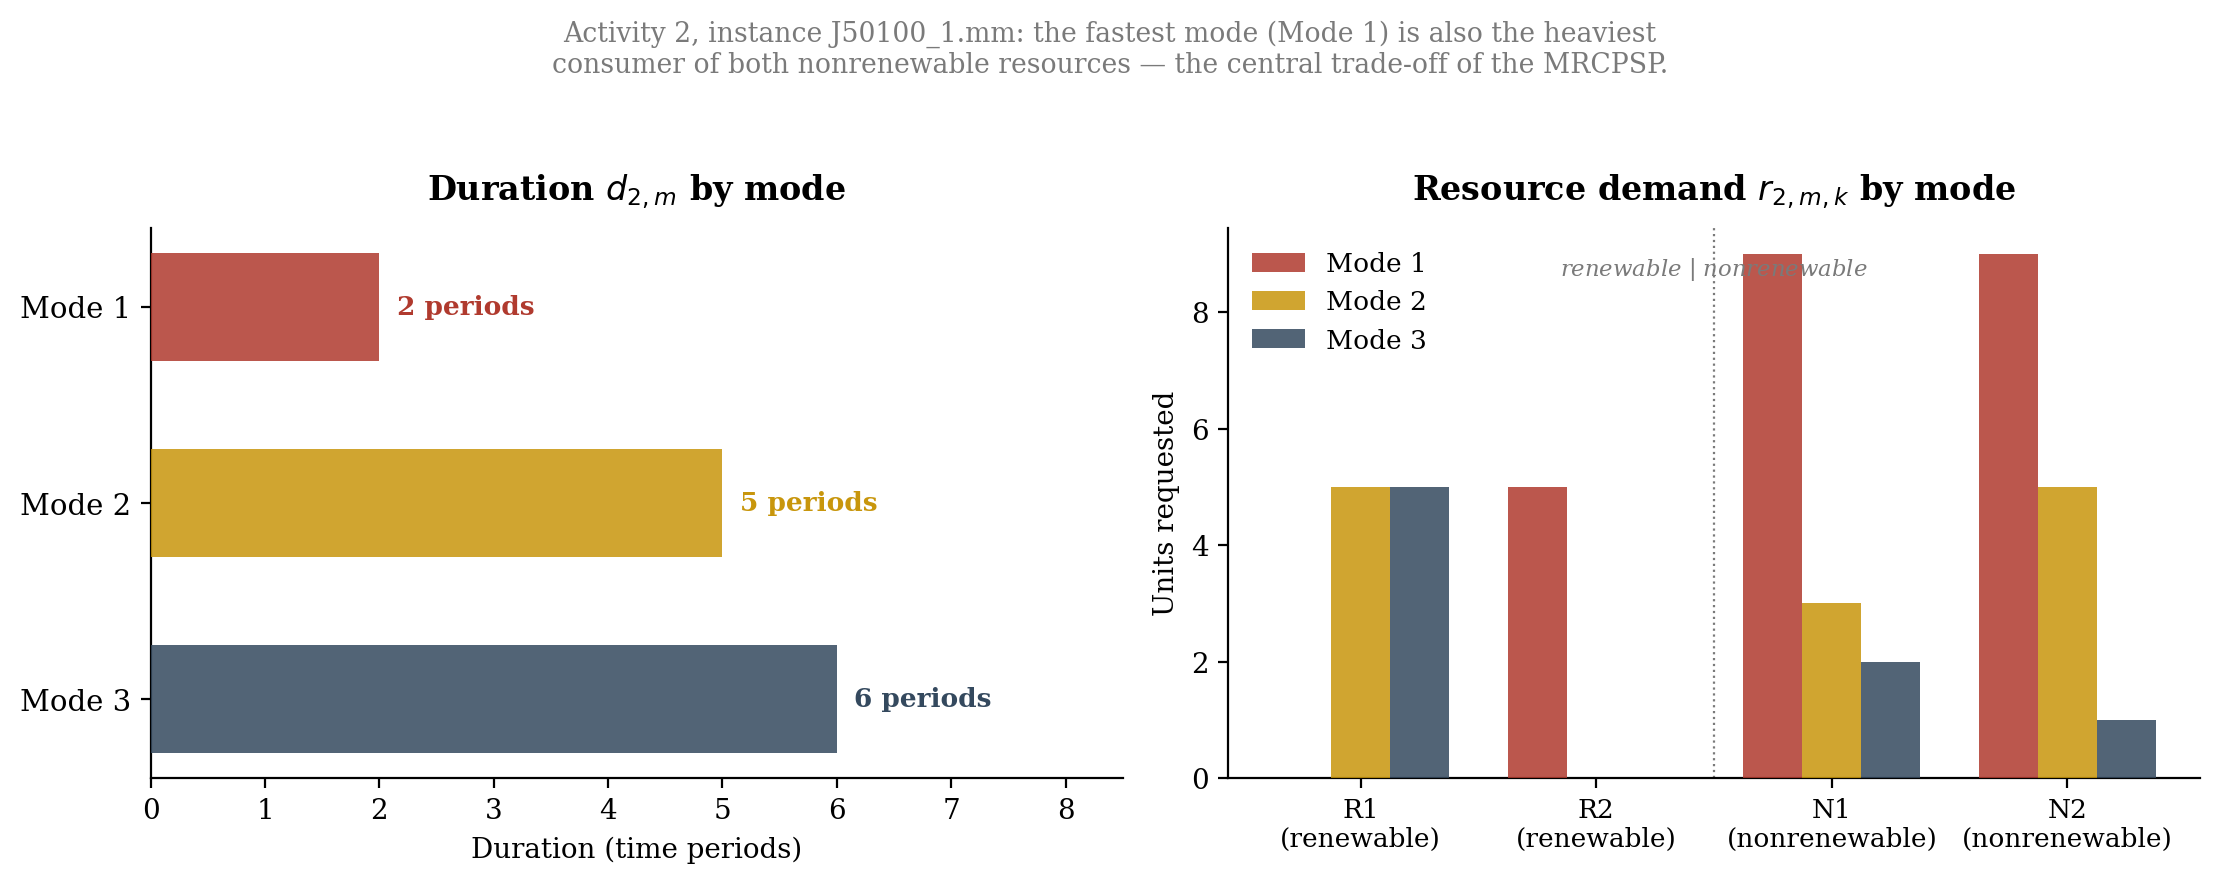
\includegraphics[width=0.95\textwidth]{img/mode-tradeoff.png}
  \caption[Duration vs.\ resource trade-off across modes]{The duration
  vs.\ resource-consumption trade-off across the three modes of activity~2
  in the excerpt above. Left: mode~1 is the fastest. Right: mode~1 is also
  the heaviest consumer of both nonrenewable resources N1 and N2, while
  modes~2 and~3 trade additional duration for a lighter nonrenewable
  footprint: the mode-choice trade-off central to the MRCPSP
  (Section~\ref{subsec:problem-statement}).}
  \label{fig:mode-tradeoff}
\end{figure}

The header fixes the total number of jobs, including the two zero-duration
dummy activities that act as a unique source and sink for the
activity-on-node network of Section~\ref{subsec:cpm}, and the number of
renewable and nonrenewable resource types. The precedence block lists, for
every activity, its number of modes and its immediate successors, which
together define the precedence graph. The requests/durations block then
gives, for every mode $m \in \mathcal{M}_i$ of activity $i$, the duration $d_{im}$ and
the per-period requirement $r_{imk}$ of every resource $k$: choosing a mode
fixes both quantities simultaneously, so a shorter mode (e.g.\ activity~2,
mode~1, duration~2) typically demands more of one resource and less of
another than a longer mode (mode~3, duration~6); this is the mode-choice
trade-off central to the MRCPSP (Section~\ref{subsec:problem-statement}).
Finally, the availabilities block gives the per-period capacity of each
renewable resource and the total project budget of each nonrenewable
resource.

\changedB{When an instance is loaded, the parser produces a model object exposing the
activities, their modes (with per-mode durations and resource requirements),
the precedence relations and the capacities of both resource classes
programmatically; this is the representation queried directly by the GP
terminals and the schedule-generation scheme described in
Chapter~\ref{chap:approach}.}

\subsection{Instance characterisation indicators}
\label{subsec:indicators}

To produce a controlled spread of instance difficulty, MMLIB instances are
generated to target specific values of three pre-existing project- and
resource-characterisation indicators (order strength, resource factor and
resource strength) which Van Peteghem and Vanhoucke adopt when
constructing the dataset~\cite{vanpeteghem2014}.

\textbf{Order strength (OS)} is the density of the precedence graph. Let
$V' = V \setminus \{0, n+1\}$ be the non-dummy activities and let $\mathcal{P}
\subseteq V' \times V'$ be the transitive closure of the precedence edge set
$E$ (Section~\ref{subsec:rcpsp-model}) restricted to $V'$, i.e. $\mathcal{P}$
contains every directly \emph{and} transitively implied precedence relation
between non-dummy activities. OS is then $|\mathcal{P}|$ divided by the
maximum possible number of relations among $n$ activities,
\[
  \mathrm{OS} = \frac{|\mathcal{P}|}{n(n-1)/2}.
\]
A low OS means many activities can run in parallel, so resource conflicts
dominate scheduling decisions; a high OS means the project is largely
serial, so precedence dominates.

\textbf{Resource factor (RF)} measures how many of the available resource
types each activity actually consumes. For renewable resources it is the
fraction of (activity, mode, resource) triples with a strictly positive
requirement,
\[
  \mathrm{RF}_{\mathcal{R}^{\rho}} =
  \frac{1}{n\,|\mathcal{R}^{\rho}|}
  \sum_{i=1}^{n} \sum_{m \in \mathcal{M}_i} \sum_{k \in \mathcal{R}^{\rho}}
  \mathds{1}\!\left[r^{\rho}_{imk} > 0\right],
\]
\changed{where $\mathds{1}[\cdot]$ is the indicator function, equal to $1$
when the bracketed condition holds and $0$ otherwise, and the notation for
activities, modes, resources and requirements is that of
Section~\ref{subsec:mrcpsp-model},}
with $\mathrm{RF}_{\mathcal{R}^{\nu}}$ defined analogously over the nonrenewable
resources $\mathcal{R}^{\nu}$. $\mathrm{RF}=1$ means every activity requests
every resource type; $\mathrm{RF}=0$ means no activity requests any resource
of that class.

\textbf{Resource strength (RS)}, following Van Peteghem and Vanhoucke's
definition~\cite{vanpeteghem2014} (their Eq.\ (8), stated there for the
nonrenewable case and extended here per resource $k$), measures how tight the
resource availability is relative to demand,
\[
  RS^{\rho}_k = \frac{a^{\rho}_k - r^{\rho}_{k,\min}}{r^{\rho}_{k,\max} - r^{\rho}_{k,\min}},
  \qquad
  RS^{\nu}_k = \frac{a^{\nu}_k - r^{\nu}_{k,\min}}{r^{\nu}_{k,\max} - r^{\nu}_{k,\min}},
\]
where $a^{\rho}_k$ ($a^{\nu}_k$) is the availability of resource $k$ (denoted
$R^{\rho}_k$/$R^{\nu}_k$ in Section~\ref{subsec:mrcpsp-model}'s notation),
$r^{\rho}_{k,\min}$ ($r^{\nu}_{k,\min}$) is
the minimum amount of $k$ that is needed for the instance to remain feasible
at all\changed{, a quantity computable directly from the instance data:
for a renewable resource it is the largest per-period demand no mode
choice can avoid, $r^{\rho}_{k,\min} = \max_{i} \min_{m \in \mathcal{M}_i}
r^{\rho}_{imk}$ (with less capacity than this, some activity could not be
executed in any mode), and for a nonrenewable resource it is the total
consumption when every activity uses its cheapest mode,
$r^{\nu}_{k,\min} = \sum_{i} \min_{m \in \mathcal{M}_i} r^{\nu}_{imk}$},
and $r^{\rho}_{k,\max}$ ($r^{\nu}_{k,\max}$) is the peak (renewable)
or total (nonrenewable) demand for $k$ when every activity is scheduled as
early as possible, ignoring resource constraints. $RS$ close to $0$ indicates
a tightly resource-constrained instance, while $RS$ close to $1$ indicates
that the resource is effectively unconstrained. In MMLIB, OS, RF and RS are
each set to one of a small number of target levels (typically
$0.25$/$0.5$/$0.75$) when generating instances, which is what gives the
library its systematic coverage of the instance space.

\begin{figure}[htbp]
  \centering
  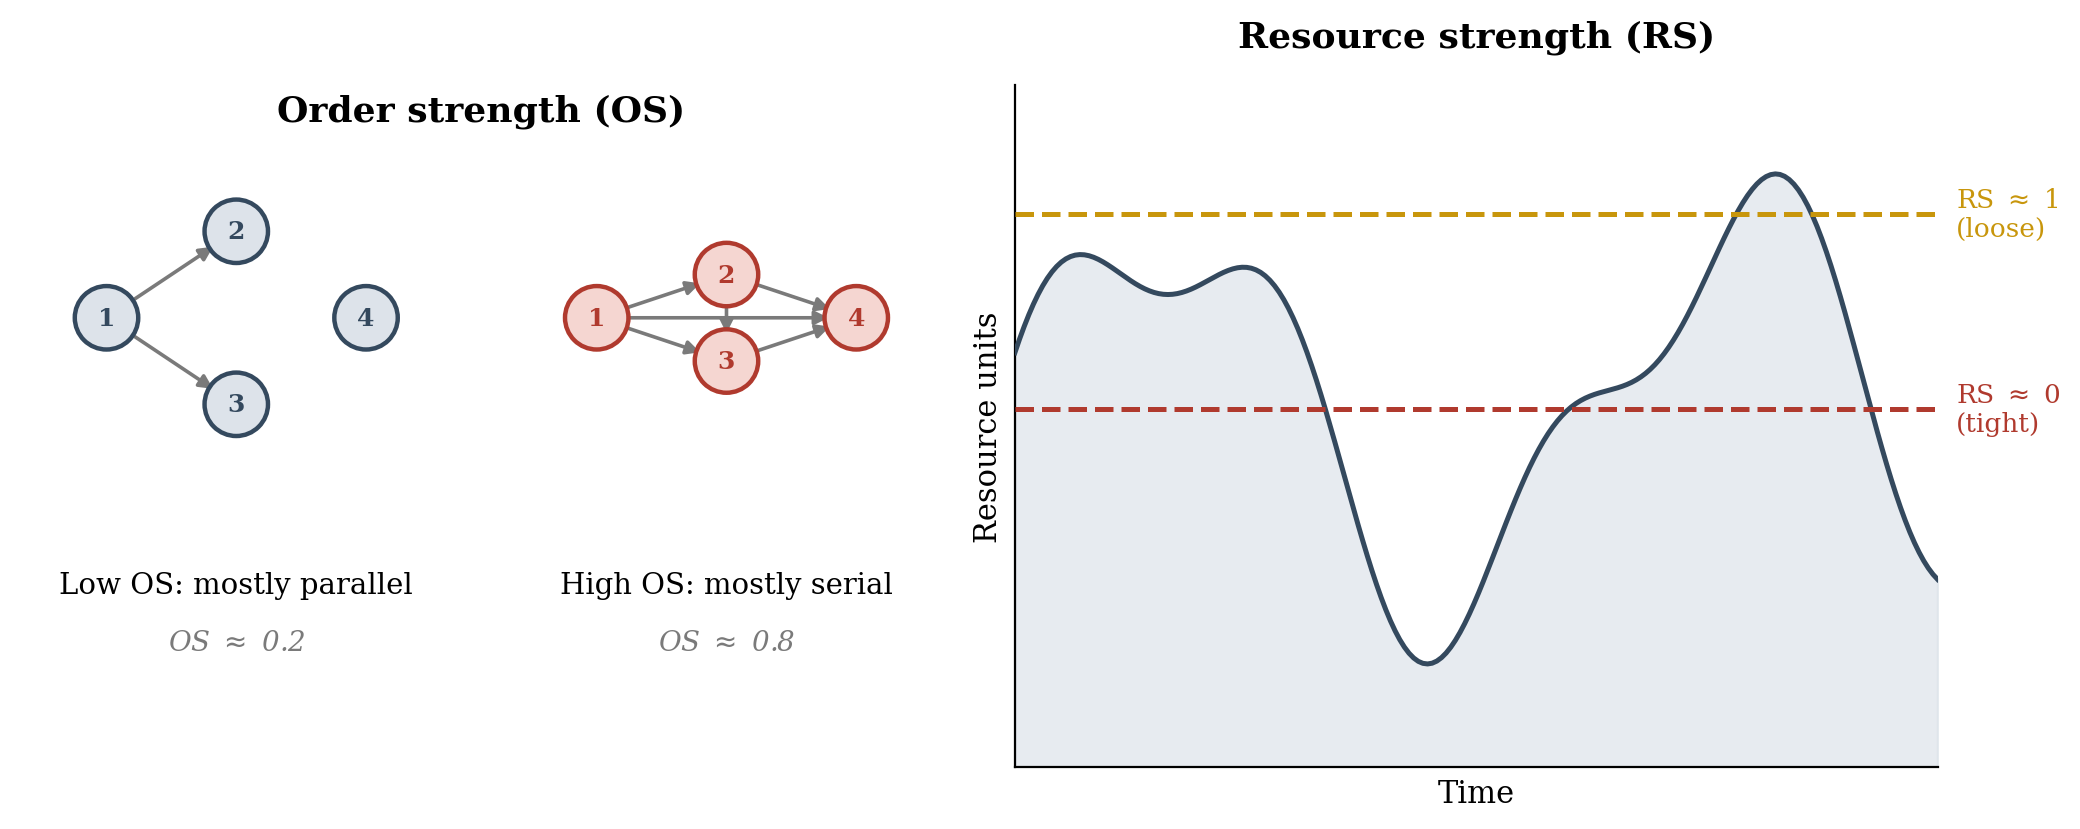
\includegraphics[width=0.95\textwidth]{img/instance-indicators.png}
  \caption[Order strength and resource strength, illustrated]{Order strength
  (OS) and resource strength (RS) illustrated on small synthetic examples.
  Left: a low-OS precedence graph (many parallel activities) versus a
  high-OS graph (a near-serial chain). Right: \changed{the solid curve is
  the aggregate demand for one renewable resource over time under an
  earliest-start schedule; the two dashed horizontal lines are two
  alternative per-period availability levels for the same demand profile.
  An availability well above the demand peak gives a loose instance
  ($\mathrm{RS}\approx 1$), an availability close to the unavoidable
  minimum a tight one ($\mathrm{RS}\approx 0$).} Resource factor (RF) is
  omitted as it is a simple counting indicator with no useful graphical
  analogue.}
  \label{fig:instance-indicators}
\end{figure}

%==============================================================================
\section{Schedule quality evaluation metrics}
\label{sec:eval-metrics}
%==============================================================================

A \emph{schedule} for an MRCPSP instance assigns every activity a mode
$m \in \mathcal{M}_i$ and a start time, and is \emph{feasible} if it satisfies the
three constraint classes of Section~\ref{subsec:problem-statement}:
precedence, per-period renewable-resource availability, and total
nonrenewable-resource budgets. Only feasible schedules are considered; the
schedule-generation scheme used throughout this thesis (and by the baseline)
constructs feasible schedules by design, so feasibility itself is not used as
a ranking criterion; schedules are compared purely on quality.

The primary quality measure is the \emph{makespan} $C_{\max}$, the completion
time of the sink activity, as already defined in
Section~\ref{subsec:cpm}. Because $C_{\max}$ depends strongly on instance
size, it cannot be compared directly across instances of different $n$, OS,
RF or RS. Following standard practice in the (M)RCPSP
literature~\cite{kolisch1997,vanpeteghem2014}, $C_{\max}$ is therefore
normalised against an instance-specific lower bound before being aggregated.

\textbf{CPM-based lower bound.} For instance $i$, let
$d_{i}^{\min} = \min_{m \in \mathcal{M}_i} d_{im}$ be the duration of its shortest
mode. Applying the forward CPM recursion of
Section~\ref{subsec:passes}, equations~\eqref{eq:es}--\eqref{eq:ef}, with
$d_{i}^{\min}$ in place of $d_i$ and \emph{ignoring all resource
constraints} gives the earliest finish (EF) time of the sink activity, denoted
$\mathrm{CPM}_{\mathrm{EF}}(i)$. Since both the resource constraints and the
choice of (possibly longer) modes are relaxed, $\mathrm{CPM}_{\mathrm{EF}}(i)$
is a valid, though generally not tight, lower bound on $C_{\max}(i)$ for
any feasible schedule of instance $i$, and depends only on the instance, not
on the algorithm being evaluated.

\textbf{Relative deviation.} The quality of a schedule with makespan
$C_{\max}(i)$ on instance $i$ is reported as its percentage deviation from
this lower bound,
\[
  \mathrm{dev}(i) \;=\; \frac{C_{\max}(i) - \mathrm{CPM}_{\mathrm{EF}}(i)}{\mathrm{CPM}_{\mathrm{EF}}(i)} \times 100\%.
\]
Averaging $\mathrm{dev}(i)$ over a set of instances (training, validation or
test) gives the \emph{Average Relative Deviation} (ARD\%), the single number
used both as the GP fitness function during training
(Section~\ref{subsec:problem-statement}, Chapter~\ref{chap:approach}) and as
the headline figure for comparing configurations and reporting results in
Chapter~\ref{chap:experiments}.

\textbf{Statistical comparison.} Because $\mathrm{dev}(i)$ is computed for
every algorithm configuration on the same instances, two configurations can
be compared instance-by-instance using a paired, non-parametric Wilcoxon
signed-rank test on the per-instance deviations. Chapter~\ref{chap:experiments}
reports such comparisons against the baseline using a one-sided test (the
alternative hypothesis being that the proposed configuration's deviations are
\emph{lower}), marking improvements as significant at the $p<0.05$ and
$p<0.10$ levels.

\chapter{Proposed approach and novelty}
\label{chap:approach}

This chapter defines the algorithmic starting point against which every
proposed modification in Chapter~\ref{chap:experiments} is measured. It
fixes, in detail, the exact baseline configuration, representation,
decoding procedure, and operators shared by the baseline and every
extension evaluated later, so that Chapter~\ref{chap:experiments}'s
comparisons isolate the effect of each proposed change rather than any
incidental difference in the surrounding machinery.

\section{Definition of the baseline algorithm}
\label{sec:baseline-definition}

The baseline used for comparison is the Genetic Programming Hyper-Heuristic
(GPHH) method for MRCPSP introduced by Tian, Mei, and Zhang~\cite{Tian2024GPHH},
presented at the 2024 IEEE Congress on Evolutionary Computation. \changed{The
authors' own implementation, available at
\url{https://github.com/TianYuanSX/GP\_MRCPSP\_CEC2024}, is used unmodified
as the baseline throughout this thesis. The following subsections describe
its components in turn: the core idea, the individual representation and
its terminal sets, the schedule construction procedure, the fitness
evaluation, and the evolutionary operators and parameters.} GPHH is
evaluated on the same MMLIB50 and MMLIB100 benchmark sets as the proposed
algorithm, making it a directly comparable starting point.

\subsection{Core idea: evolving heuristics rather than schedules}

GPHH belongs to the class of hyper-heuristic methods: instead of searching for good schedules directly, it uses Genetic Programming to automatically evolve scheduling priority rules.
Each evolved rule is an executable symbolic expression that, when applied inside a Schedule Generation Scheme (SGS), determines which activity to schedule next and in which execution mode.
The GP search operates at the level of rules, not solutions; once the best rule has been found on a training set of instances, it is applied to new instances without any further search.
\changed{Figure~\ref{fig:gphh-architecture} gives an overview of the whole pipeline; the remaining subsections describe its stages in turn.}

\begin{figure}[t]
  \centering
  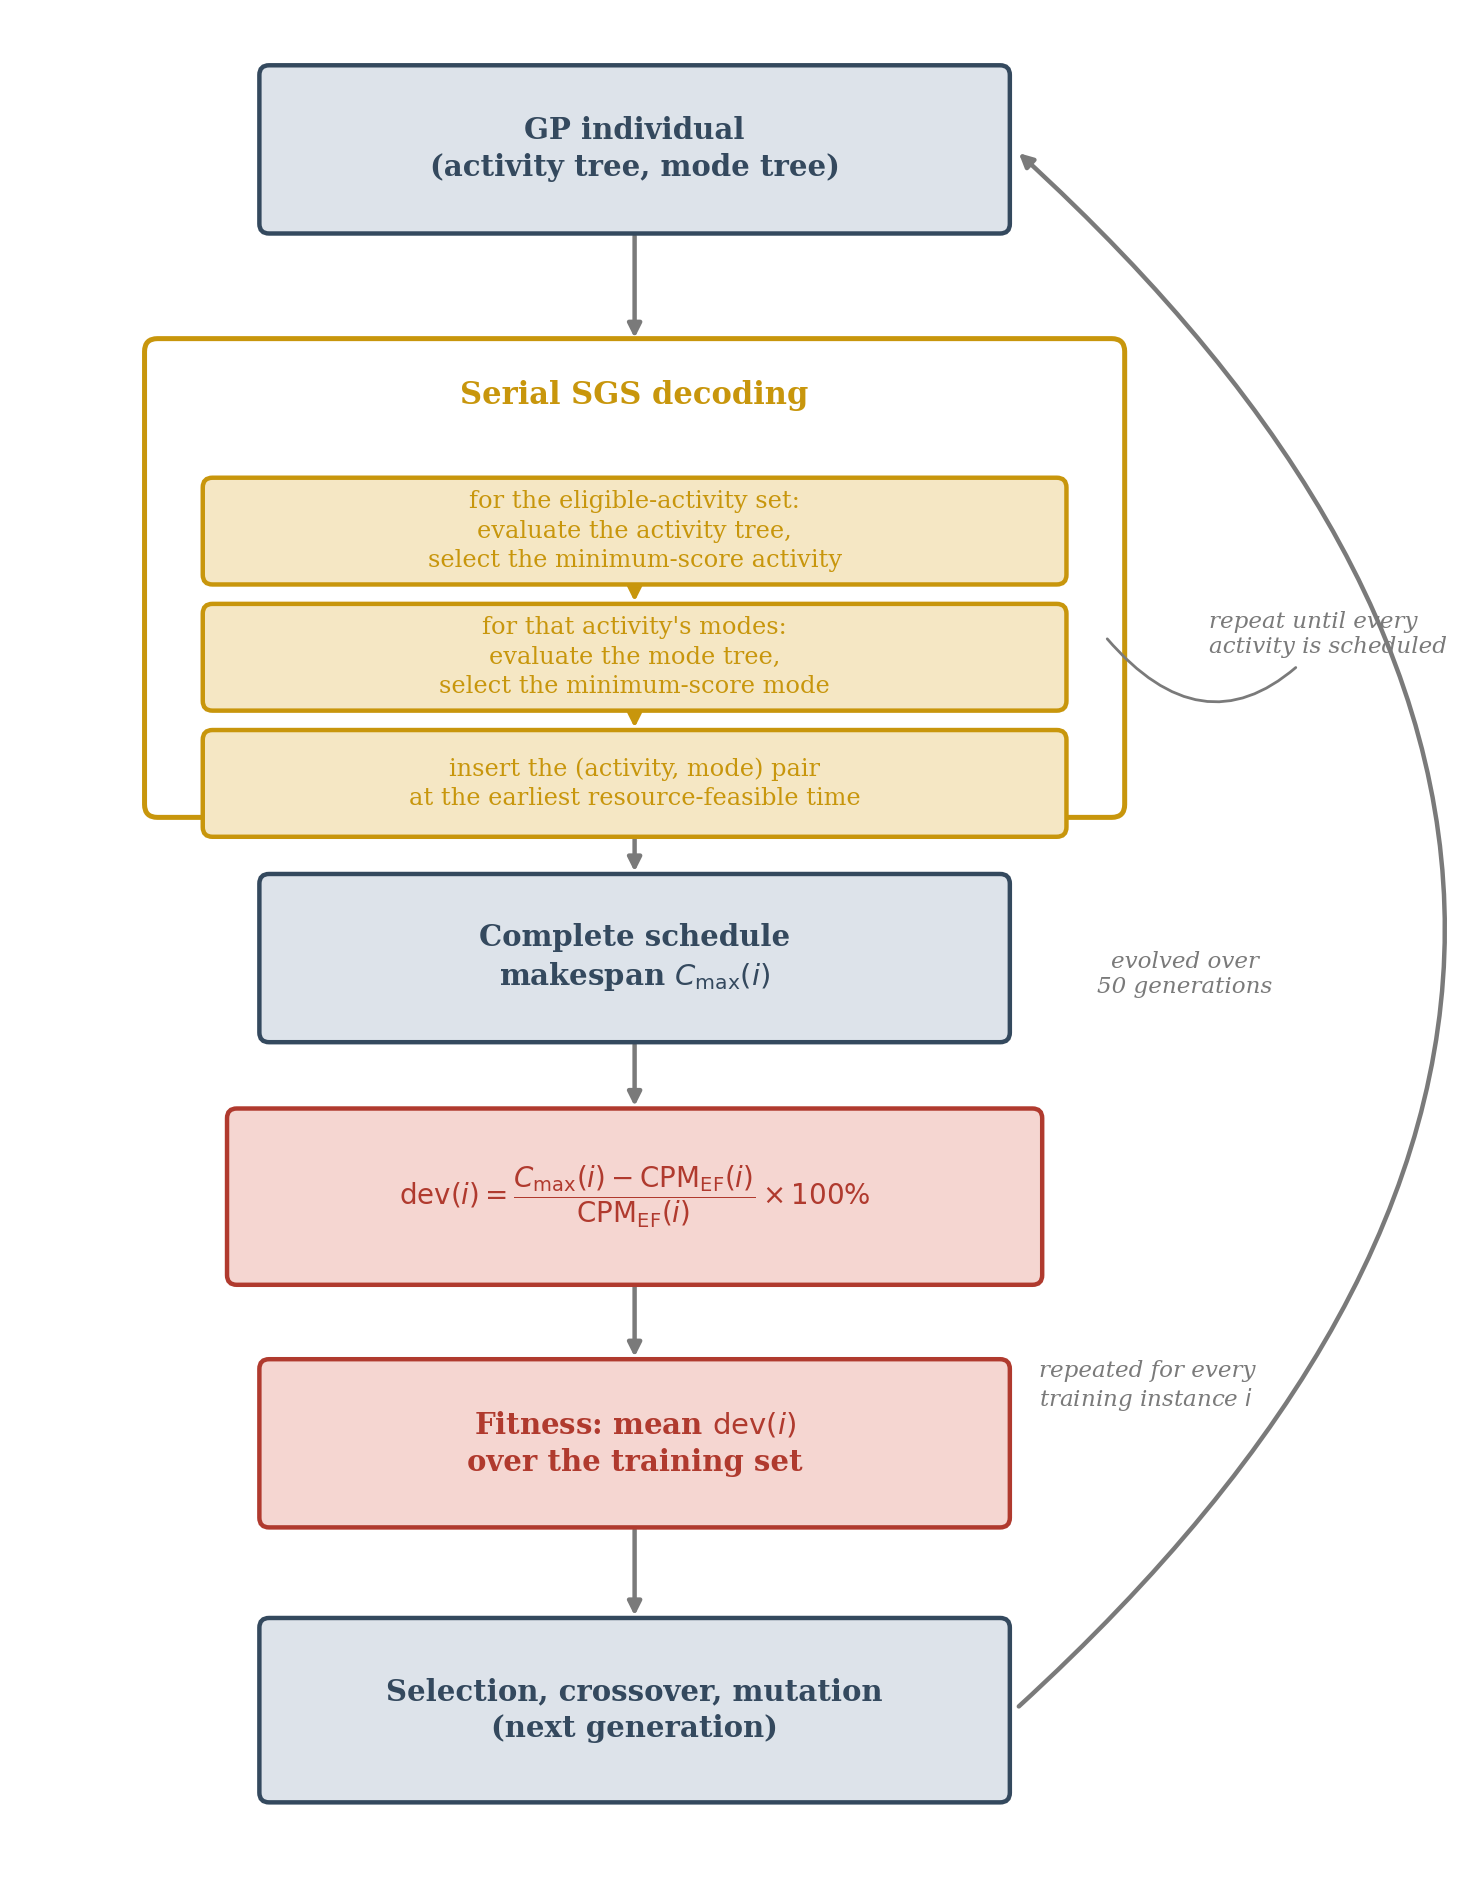
\includegraphics[width=0.78\textwidth]{img/gphh-architecture.png}
  \caption[The baseline GPHH pipeline]{Overview of the baseline GPHH
  pipeline: a multi-tree individual drives the serial SGS decoding loop to
  produce a complete schedule, whose deviation from the CPM lower bound is
  averaged over the training set to obtain the individual's fitness, which
  in turn drives selection, crossover and mutation for the next generation.
  The remaining subsections of this section detail each stage.}
  \label{fig:gphh-architecture}
\end{figure}

\subsection{Individual representation: multi-tree GP}
\label{subsec:individual-representation}

Each individual in the GP population is a pair of symbolic expression trees evolved simultaneously.
The \emph{activity tree} computes a numeric priority value for each eligible activity; the activity with the lowest value is selected next.
The \emph{mode tree} then computes a priority value for each available execution mode of the selected activity; again the mode with the lowest value is assigned.
This two-tree structure (referred to as \texttt{activity\_first} in the implementation) separates the activity-selection and mode-selection decisions into independently evolved sub-rules.

Both trees are constructed from a shared \textbf{function set}: \texttt{add}, \texttt{sub}, \texttt{mul}, \texttt{div} (protected against division by zero), \texttt{min}, and \texttt{max}.
The \textbf{terminal sets} differ between the two trees to reflect the information relevant at each decision stage\changed{, and are defined precisely in Tables~\ref{tab:activity-terminals} and~\ref{tab:mode-terminals}.
In the definitions, $j$ denotes the candidate activity, $\mathcal{M}_j$ its set of modes, $d_{jm}$ the duration of mode $m$, $\mathcal{K}$ the set of resource types, $r_{jmk}$ the requirement of mode $m$ for resource $k \in \mathcal{K}$, and $d^{\min}_j = \min_{m \in \mathcal{M}_j} d_{jm}$ the shortest duration available to activity $j$; $P_j$ and $S_j$ are the sets of immediate predecessors and successors of $j$ (Section~\ref{subsec:passes}), and $\bar{P}_j$ and $\bar{S}_j$ the corresponding transitive closures (all direct and indirect predecessors and successors).
The activity-tree terminals are static: they are computed once per instance, before decoding starts, with the four CPM dates obtained from one forward and backward pass (Section~\ref{subsec:passes}) on the resource-relaxed instance with every activity at its shortest duration $d^{\min}_j$.
Of the mode-tree terminals, only EFFT is dynamic, i.e.\ depends on the state of the partially built schedule at the moment the rule is queried; the remaining terminals are properties of the candidate mode or of the instance.}

\changedC{The order just described, select the activity first, then its
mode, is only one way to organise the decision, and Tian et
al.~\cite{Tian2024GPHH} define three variants, called \emph{GP decision
strategies} throughout this thesis; every experiment of
Chapter~\ref{chap:experiments} is run under each of the three.
Under \emph{activity-first} (the variant described above), the activity
tree scores every eligible activity, the lowest-scoring activity is
selected, and the mode tree then scores only that activity's modes to pick
one. Under \emph{mode-first}, the order is reversed: the mode tree first
commits a mode for every eligible activity (each activity's
lowest-scoring mode), and the activity tree then chooses among the
eligible activities, each already seen in its committed mode; the chosen
activity is scheduled in that mode. Because the mode is fixed before the
activity decision, the mode-first activity tree drops the across-modes
aggregates of Table~\ref{tab:activity-terminals} (the
\texttt{avg/max/min\_task\_duration} and \texttt{RReq\_m} terminals),
which would be redundant in that context. Under \emph{simultaneous},
finally, the individual is a single integrated tree rather than a pair:
it draws on the combined terminal vocabulary of both tables and scores
every eligible (activity, mode) pair jointly, and the lowest-scoring pair
is scheduled. Activity-first and mode-first therefore both evolve two
coupled trees and differ in which decision constrains which, while
simultaneous evolves one rule over the joint decision space, a
distinction that Section~\ref{subsec:nr-eval} shows to matter.}

\begin{table}[htbp]
  \centering
  \caption[Terminal set of the activity tree]{\changed{Terminal set of the
  activity tree. All terminals are computed
  once per instance before decoding.}}
  \label{tab:activity-terminals}
  \small
  \begin{tabularx}{\textwidth}{@{}l X@{}}
    \toprule
    \textbf{Terminal} & \textbf{Definition} \\
    \midrule
    \texttt{PC} & $|P_j|$ \\
    \texttt{TPC} & $|\bar{P}_j|$ \\
    \texttt{SC} & $|S_j|$ \\
    \texttt{TSC} & $|\bar{S}_j|$ \\
    \texttt{GRPW} & $d^{\min}_j + \sum_{i \in S_j} d^{\min}_i$
      (Greatest Rank Positional Weight) \\
    \texttt{GRPW\_all} & $d^{\min}_j + \sum_{i \in \bar{S}_j} d^{\min}_i$ \\
    \texttt{ES}, \texttt{EF}, \texttt{LS}, \texttt{LF} & $EST_j$, $EFT_j$,
      $LST_j$, $LFT_j$ (Section~\ref{subsec:passes}),
      computed on the resource-relaxed instance with durations $d^{\min}_j$ \\
    \texttt{avg\_task\_duration} &
      $\frac{1}{|\mathcal{M}_j|} \sum_{m \in \mathcal{M}_j} d_{jm}$ \\
    \texttt{max/min\_task\_duration} &
      $\max_{m \in \mathcal{M}_j} d_{jm}$,\;
      $\min_{m \in \mathcal{M}_j} d_{jm}$ \\
    \texttt{avg\_RReq\_m} &
      $\frac{1}{|\mathcal{M}_j|\,|\mathcal{K}|}
       \sum_{m \in \mathcal{M}_j} \sum_{k \in \mathcal{K}} r_{jmk}$ \\
    \texttt{max/min\_RReq\_m} &
      $\max_{m \in \mathcal{M}_j,\, k \in \mathcal{K}} r_{jmk}$,\;
      $\min_{m \in \mathcal{M}_j,\, k \in \mathcal{K}} r_{jmk}$ \\
    \bottomrule
  \end{tabularx}
\end{table}

\begin{table}[t]
  \centering
  \caption[Terminal set of the mode tree]{\changed{Terminal set of the mode
  tree, evaluated for a candidate mode
  $m$ of the selected activity $j$. Only \texttt{EFFT} depends on the
  current decoding state.}}
  \label{tab:mode-terminals}
  \small
  \begin{tabularx}{\textwidth}{@{}l X@{}}
    \toprule
    \textbf{Terminal} & \textbf{Definition} \\
    \midrule
    \texttt{task\_duration} & $d_{jm}$ \\
    \texttt{EFFT} & $\mathrm{EFFT}_{jm} = \min_{t \in F_{jm}} (t + d_{jm})$,
      where $F_{jm}$ is the set of feasible start times of $j$ in mode $m$
      under the current partial schedule; the mode-selection rule of Lova,
      Tormos and Barber~\cite{lova2006mrcpsp} \\
    \texttt{RR} & $|\{\,k \in \mathcal{K} : r_{jmk} > 0\,\}|$ \\
    \texttt{GRD} & $d_{jm} \cdot |\{\,k \in \mathcal{K} : r_{jmk} > 0\,\}|$ \\
    \texttt{avg\_RReq} &
      $\frac{1}{|\mathcal{K}|} \sum_{k \in \mathcal{K}} r_{jmk}$ \\
    \texttt{max/min\_RReq} &
      $\max_{k \in \mathcal{K}} r_{jmk}$,\;
      $\min_{k \in \mathcal{K}} r_{jmk}$ \\
    \texttt{avg\_ResCap} &
      $\frac{1}{|\mathcal{K}|} \sum_{k \in \mathcal{K}} R_k$
      (instance constant; $R_k$ is resource $k$'s capacity) \\
    \texttt{max/min\_ResCap} &
      $\max_{k \in \mathcal{K}} R_k$,\;
      $\min_{k \in \mathcal{K}} R_k$ \\
    \bottomrule
  \end{tabularx}
\end{table}

\subsection{Schedule construction via SGS}
\label{subsec:sgs-construction}

\changedB{At runtime the evolved rule pair drives the serial SGS of
Algorithm~\ref{alg:serial-sgs} (Section~\ref{subsec:sgs}), with one
multi-mode extension.}
\changedB{The activity tree plays the role of the priority rule $\pi$: at
each step it is evaluated for every eligible activity (those whose
predecessors have all been completed) and the activity $j^{*}$ with the
minimum score is chosen. The selection of $j^{*}$ is followed by one extra
step that the single-mode statement of Algorithm~\ref{alg:serial-sgs} does
not need: the mode tree is evaluated for every available mode
$m \in \mathcal{M}_{j^{*}}$ and the mode with the minimum score is
assigned.}
The activity is inserted into the schedule at the earliest time at which all renewable resource requirements of the chosen mode are satisfied.
This process repeats until all activities are scheduled.

\subsection{Fitness evaluation}
\label{subsec:fitness-evaluation}

Each individual is evaluated on a fixed \emph{training set} of MRCPSP instances drawn from the MMLIB benchmark library.
\changed{The reference value for each instance is its \emph{CPM lower bound}
$\mathrm{CPM}_{\mathrm{EF}}(i)$: the critical-path length of instance $i$,
computed by one CPM pass (Section~\ref{subsec:passes}) with all resource
constraints relaxed and every activity at its shortest mode duration.
Since removing constraints and shortening activities can only decrease the
optimal makespan, no feasible schedule can finish earlier than this bound.}
For each training instance $i$ the rule pair constructs a schedule via the SGS and the deviation of the resulting makespan from the CPM lower bound is recorded as
\[
    \mathrm{dev}(i) \;=\; \frac{C_{\max}(i) - \mathrm{CPM}_{\mathrm{EF}}(i)}{\mathrm{CPM}_{\mathrm{EF}}(i)} \times 100\%.
\]
The fitness of the individual is the mean deviation across all training instances.
A separate \emph{validation set} is used at the end of each generation to monitor generalisation, and a held-out \emph{test set} provides the final performance figure.

\subsection{Evolutionary operators and parameters}
\label{subsec:evolutionary-operators}

Selection uses tournament selection with tournament size~7.
Crossover applies one-point subtree exchange at rate~0.8 with the standard Koza-style 90/10 bias toward internal (non-terminal) over leaf nodes as the crossover point, favouring the exchange of larger structural subtrees over trivial leaf swaps.
Mutation applies the same 90/10 internal-over-leaf bias to its replacement point, at rate~0.15, again favouring structural change over simple leaf substitution.
Both operators enforce a hard tree-depth limit of~8 after application.
Initial trees are generated by the half-and-half method to depths between~2 and~6.
The default configuration uses a population of 1\,000 individuals, 50 generations, and 10 elite individuals carried forward unchanged each generation.

\section{The proposed algorithm}
\label{sec:proposed-algorithm}

\changedB{This section defines the three proposed extensions of the
baseline: non-renewable resource terminals
(Section~\ref{subsec:nr-terminals-definition}), epsilon-lexicase selection
(Section~\ref{subsec:lexicase-definition}), and critical-path-guided local
search (Section~\ref{subsec:localsearch-definition}).
Section~\ref{sec:parameter-sensitivity} then documents the exploratory
screening through which they were selected and the alternatives that were
rejected.}
Non-renewable resource terminals are presented first and in the most
detail, since they are this thesis's central, most novel proposed
contribution: unlike lexicase selection and critical-path local search,
which adapt existing evolutionary-computation mechanisms to this problem,
NR terminals close a genuine, previously unaddressed information gap in
the GPHH terminal set itself.

\subsection{Non-renewable resource terminals}
\label{subsec:nr-terminals-definition}

The baseline's terminal set (Section~\ref{subsec:individual-representation})
gives the GP visibility into precedence structure and renewable-resource
demand, but nothing about non-renewable (NR) resource state: no terminal
tells the evolving rule how much of the project's total NR budget remains,
or how much a candidate mode would spend against it. This is a genuine
information gap, not a hypothetical one, since mode choice is exactly the
decision that trades duration and renewable-resource use against NR
consumption: a rule with no NR signal at all can only manage the NR budget
by accident. The proposed extension closes this
gap with three additions to the terminal set, computed from each resource's
initial and remaining stock and each task's per-mode demand.
\changed{In the definitions below, $\mathcal{R}^{\nu}$ is the set of NR
resource types, $R^{\nu}_k$ the initial budget of resource $k$,
$\mathrm{rem}_k$ its remaining stock at the current decision point (initial
budget minus the consumption of every already-committed activity/mode
pair), $r^{\nu}_{jmk}$ the demand of the candidate activity $j$ in mode
$m$, and $U$ the set of not-yet-scheduled activities:}

\begin{itemize}
  \item \textbf{\texttt{NR\_STOCK\_RATIO}} (activity and integrated trees):
  the minimum, across all NR resource types, of remaining stock divided by
  initial stock,
  \changed{\[
    \texttt{NR\_STOCK\_RATIO} \;=\;
    \min_{k \in \mathcal{R}^{\nu}} \frac{\mathrm{rem}_k}{R^{\nu}_k},
  \]}
  a single aggregated scalar answering ``how much of the
  project's NR budget is left right now.'' One aggregated value rather than
  one terminal per resource type is used deliberately, so that the same
  tree remains well-defined regardless of how many NR resource types a
  given instance happens to have.
  \item \textbf{\texttt{NR\_MODE\_DEMAND\_RATIO}} (mode tree only): the
  maximum, across NR resource types, of a candidate mode's NR demand
  divided by remaining stock,
  \changed{\[
    \texttt{NR\_MODE\_DEMAND\_RATIO} \;=\;
    \max_{k \in \mathcal{R}^{\nu}} \frac{r^{\nu}_{jmk}}{\mathrm{rem}_k}
  \]
  (a zero-demand resource contributes $0$; an exhausted one,
  $\mathrm{rem}_k \le 0$ with positive demand, contributes a large penalty
  constant so such modes rank last).} This is the most directly decision-relevant
  of the three, since mode choice is precisely what trades duration against
  NR consumption, and demand relative to \emph{remaining} (not initial)
  stock matches how the simulator already gates mode eligibility on
  currently available resources.
  \item \textbf{\texttt{NR\_BUDGET\_PRESSURE}} (activity and integrated
  trees): a forward-looking feasibility-risk proxy, the minimum, across NR
  resource types, of remaining stock minus the sum of every not-yet-scheduled
  activity's cheapest-mode demand for that resource, normalised by initial
  stock,
  \changed{\[
    \texttt{NR\_BUDGET\_PRESSURE} \;=\;
    \min_{k \in \mathcal{R}^{\nu}}
    \frac{\mathrm{rem}_k - \sum_{i \in U} \min_{m \in \mathcal{M}_i} r^{\nu}_{imk}}{R^{\nu}_k}.
  \]}
  Unlike the other two terminals, which describe the present, this
  one estimates whether the \emph{remainder} of the project can still be
  completed at all under the current NR budget.
\end{itemize}

Because these terminals are only meaningful on instances that still carry
their non-renewable resources, this extension additionally changes which
instances are loaded. \changedB{The baseline pipeline follows the paper's
own preprocessing: as each MMLIB instance is read, every non-renewable
resource is stripped from it, leaving the modes, durations and renewable
constraints intact but removing the NR budgets entirely, so the baseline
in fact runs on a renewable-only relaxation of the original MRCPSP.} For
this extension, NR-preserving instances are read directly instead
(\texttt{keep\_non\_renewable=True}), so the terminals reflect a genuine
resource constraint rather than a placeholder. Every other element of the
representation, function set, decoding procedure and fitness computation
(Sections~\ref{subsec:individual-representation}--\ref{subsec:fitness-evaluation})
is left completely unchanged; NR terminals are a strictly additive change
to the terminal set, evaluated against a matched baseline run on the same
NR-preserving instances (\texttt{baseline\_nr}), so that any measured
difference is attributable to the terminals themselves and not to a
confound in the surrounding machinery. Section~\ref{subsec:nr-eval} reports
this extension's evaluation and finds it the strongest, most broadly
replicated result in this thesis.

\subsection{Epsilon-lexicase selection}
\label{subsec:lexicase-definition}

The second proposed extension replaces the baseline's tournament selection
(Section~\ref{subsec:evolutionary-operators}) with epsilon-lexicase
selection\changed{~\cite{spector2012lexicase,lacava2016epsilon}}, leaving
the representation, variation operators and fitness
function untouched. Where tournament selection chooses a winner by
aggregate fitness over a randomly drawn subset of the population,
epsilon-lexicase selection chooses by filtering the \emph{entire}
population down case by case: for each selection event, the training
instances are shuffled into a random order, and the candidate pool is
narrowed, one instance at a time, to whichever individuals remain within an
adaptive epsilon (0.01 times the standard deviation of that instance's
scores among the current candidates) of the best score seen on that
instance, until either a single candidate remains or every instance has
been used, at which point the survivor is drawn uniformly at random from
whatever remains. Repeating this procedure independently for each parent
needed reproduces the population-level selection pressure a GA or GP
population requires. \changed{Algorithm~\ref{alg:lexicase} states one
selection event in full.} The motivation for trying this mechanism on a
multi-instance scheduling rule is that tournament selection's
aggregate-fitness pressure can let a single generalist that is merely
adequate everywhere dominate a specialist that is excellent on a difficult
subset of instances but weak elsewhere; case-by-case elimination is
designed to preserve exactly the kind of instance-specific specialists that
aggregate fitness would discard. Section~\ref{subsec:lexicase-eval}
evaluates whether that theoretical advantage materialises\changed{;
Section~\ref{subsec:pilot-lexicase-iteration} documents the staged pilot
evidence behind this extension, including its central
qualification: a real training-fitness advantage that does not always
survive to held-out test fitness.}

\begin{algorithm}[htbp]
\caption[Epsilon-lexicase selection]{\changed{Epsilon-lexicase selection of
one parent. $s(p, i)$ denotes individual $p$'s deviation on training
instance $i$; the procedure is repeated independently for every parent
needed.}}
\label{alg:lexicase}
\begin{algorithmic}[1]
\Require population $P$, training instances $I$, scores $s(p,i)$
\State shuffle $I$ into a random order $i_1, \dots, i_{|I|}$
\State $C \gets P$ \Comment{candidate pool}
\For{$t = 1, \dots, |I|$}
  \State $b \gets \min_{p \in C} s(p, i_t)$;\quad
  $\epsilon \gets 0.01 \cdot \operatorname{std}_{p \in C} s(p, i_t)$
  \State $C \gets \{\, p \in C : s(p, i_t) \le b + \epsilon \,\}$
  \If{$|C| = 1$} \State \Return the single member of $C$ \EndIf
\EndFor
\State \Return an individual drawn uniformly at random from $C$
\end{algorithmic}
\end{algorithm}

\subsection{Critical-path-guided local search}
\label{subsec:localsearch-definition}

The third proposed extension is a \changed{Baldwinian} memetic refinement step
applied to elite individuals during training, layered on top of either
selection mechanism. Once each generation's population has been evaluated,
the top 8\% of individuals by mean training fitness are selected as elites,
and each elite's own decoded schedule (not its GP tree) is refined by a
greedy hill-climb offering three move types: a mode-reassignment move, a
precedence-respecting activity-swap move, and a resource-shift move. The
resource-shift move is where critical-path information enters: rather than
proposing an arbitrary shift and re-checking feasibility from scratch, it
uses each activity's earliest and latest start dates from the classical CPM
forward/backward pass (Section~\ref{subsec:cpm}), computed once per
instance, to restrict candidate shifts to ones that are precedence-feasible
by construction. This makes the search over candidate moves both cheaper
(no wasted feasibility checks) and more likely to find a move worth
accepting than a CPM-blind alternative would. Critically, only the elite's
\emph{recorded fitness} is overwritten with whatever improvement the
hill-climb finds; the GP tree itself, the genotype that variation and
selection operate on, is left completely unchanged. \changed{This is what
makes the mechanism Baldwinian rather than Lamarckian: in a Lamarckian
memetic algorithm the improvement found by local search would be written
back into the genotype, whereas here a tree that produces an improvable
schedule is only rewarded for that schedule's improved fitness, without
the improvement itself being encoded anywhere the GP search could inherit
or recombine it directly.}
\changed{Algorithm~\ref{alg:local-search} states the procedure in full.}
Section~\ref{subsec:localsearch-eval} evaluates this extension and finds
its benefit concentrated under parallel schedule generation, a scheme
dependence discussed there and in Chapter~\ref{chap:conclusion}.

\begin{algorithm}[htbp]
\caption[Critical-path-guided local search on elites]{\changed{Critical-path-guided
local search applied to the elite individuals of one generation.}}
\label{alg:local-search}
\begin{algorithmic}[1]
\Require evaluated population; elite fraction $8\%$; iteration limit $10$
\For{each elite individual $e$ (top $8\%$ by mean training fitness)}
  \For{each training instance}
    \State $\sigma \gets$ the schedule decoded from $e$'s rule pair
    (Section~\ref{subsec:sgs-construction})
    \For{up to $10$ iterations}
      \State propose a move: mode reassignment, precedence-respecting
      activity swap, or a resource shift whose candidate start times are
      restricted to the activity's CPM window $[EST_j, LST_j]$
      \If{the moved schedule $\sigma'$ is feasible and
          $C_{\max}(\sigma') < C_{\max}(\sigma)$}
        \State $\sigma \gets \sigma'$ \Comment{accept only strict improvements}
      \EndIf
    \EndFor
  \EndFor
  \State overwrite $e$'s recorded fitness with the refined schedules' mean
  deviation \Comment{the GP tree itself is unchanged (Baldwinian)}
\EndFor
\end{algorithmic}
\end{algorithm}
\section{Screening the candidate extensions}
\label{sec:parameter-sensitivity}

\changed{Before any candidate modification was evaluated at the scale
described in Section~\ref{sec:experimental-setup}, it was screened
cheaply: small populations (tens of individuals), few generations, and a
handful of benchmark instances, all on MMLIB50 only. At the per-run
training times reported by Tian et al.~\cite{Tian2024GPHH}, a fully
powered evaluation (population 1\,000, 50 generations, 30 seeds,
Table~\ref{tab:experimental-parameters}) of even one candidate costs
anywhere from minutes to several days per run, so screening every idea at
that scale was not feasible. The screening proceeded in three rounds, each
narrowing the field: a diagnosis-driven, graft-based
variation scheme referred to as DMGE (Section~\ref{subsec:pilot-dmge}),
a round of enriched terminal sets
(Section~\ref{subsec:pilot-terminals}), and a staged evaluation of
epsilon-lexicase selection combined with a critical-path local search
(Section~\ref{subsec:pilot-lexicase-iteration}). \changed{The three
extensions defined in Section~\ref{sec:proposed-algorithm} are what
survived this screening and were selected for the fully powered evaluation
of Chapter~\ref{chap:experiments}.} The numbers in this
section should be read as directional only, since small samples inflate
effect-size estimates; every positive pilot finding is re-examined at full
statistical power in Chapter~\ref{chap:experiments}.}

\subsection{Exploratory investigation of DMGE modifications}
\label{subsec:pilot-dmge}

\changed{The first family of screened ideas modified the GP's
\emph{variation} step. The central idea is to make variation informed rather than
blind. Two terms recur below and are used in the following fixed sense: a
\emph{diagnosis} is an automatic classification of \emph{why} an evolved
rule's schedule is poor (for example, it exhausted a non-renewable
budget), read off the schedule-construction trace; a \emph{graft} is the
insertion of a small, pre-built conditional subtree, targeted at the
diagnosed deficiency, into the rule's tree, in place of the random subtree
replacement that ordinary mutation would perform. The schemes evaluated
here were assembled from a shared toolkit of seven small, individually
switchable modifications of the exploratory codebase; each is described
below with its motivation, before the schemes that combine them.}

\changed{\textbf{Modification 1: a well-defined conditional operator.} The
exploratory codebase's \texttt{if\_else} operator (a conditional primitive
used only in this screening round, not part of the baseline function set
of Section~\ref{subsec:individual-representation}) originally evaluated
both branches unconditionally and treated any nonzero condition value as
true, so a slack value of exactly zero branched incorrectly. Modification
1 replaces it with an operator that evaluates the condition against a
well-defined \texttt{condition > 0} threshold and only then evaluates the
selected branch. This is a prerequisite for every later modification that
branches on critical-path state.}

\changed{\textbf{Modification 2: non-renewable resource visibility.} The
motivation is that no baseline terminal reflects non-renewable (NR)
resource state (the gap Section~\ref{subsec:nr-terminals-definition} later
addresses directly). Two terminals are added, both averaged over the NR
resource types $k \in \mathcal{R}^{\nu}$ with remaining stock
$\mathrm{rem}_k$ and initial budget $R^{\nu}_k$:
\begin{align*}
  \texttt{NR\_STOCK\_RATIO} &=
    \frac{1}{|\mathcal{R}^{\nu}|} \sum_{k \in \mathcal{R}^{\nu}}
    \frac{\mathrm{rem}_k}{R^{\nu}_k}
    &&\text{(activity tree)},\\
  \texttt{NR\_MODE\_DEMAND\_RATIO} &=
    \frac{1}{|\mathcal{R}^{\nu}|} \sum_{k \in \mathcal{R}^{\nu}}
    \frac{r^{\nu}_{jmk}}{\mathrm{rem}_k}
    &&\text{(mode tree).}
\end{align*}
Both return neutral values on instances without NR
resources. \changedB{This two-terminal pair is the direct precursor of the NR
terminals proposed in Section~\ref{subsec:nr-terminals-definition}: the
proposed version pulls the same underlying idea out of this toolkit,
aggregates by minimum and maximum instead of the mean, adds the third,
forward-looking \texttt{NR\_BUDGET\_PRESSURE} terminal, and applies the
result as a strictly additive change to the terminal set with no
conditional grafting logic around it.}}

\changed{\textbf{Modification 3: schedule-state and mode-flexibility
terminals.} The motivation is that the baseline rule cannot behave
differently early versus late in schedule construction, and cannot see how
much freedom an activity's mode choice offers. Five terminals are added,
writing $\mathrm{avail}_k(t)$ for the remaining capacity of renewable
resource $k$ at time $t$, $t_j$ for the candidate activity's earliest
feasible start, and $n_{\mathrm{sched}}$ for the number of already-scheduled
activities:
\begin{align*}
  \texttt{SCHEDULED\_FRACTION} &= \frac{n_{\mathrm{sched}}}{n},\\
  \texttt{NUM\_MODES} &= |\mathcal{M}_j|,\\
  \texttt{DURATION\_FLEXIBILITY} &=
    \frac{\max_{m} d_{jm} - \min_{m} d_{jm}}{\max_{m} d_{jm}},\\
  \texttt{BOTTLENECK\_RENEWABLE\_RATIO} &=
    \min_{k \in \mathcal{R}^{\rho}} \frac{\mathrm{avail}_k(t_j)}{R^{\rho}_k},\\
  \texttt{RENEWABLE\_DEMAND\_VS\_AVAILABILITY} &=
    \max_{k \in \mathcal{R}^{\rho}} \frac{r^{\rho}_{jmk}}{\mathrm{avail}_k(t_j)},
\end{align*}
the last two capturing how free the tightest renewable resource still is
at the activity's start and a mode's demand relative to what is available
at the current decision moment.}

\changed{\textbf{Modification 4: critical-path-preserving mutation.} Once
Modification 1 makes critical-path-conditioned branches meaningful,
ordinary mutation is as likely to destroy such a branch as any other
subtree. This modification scans a tree before mutating it, marks every
node whose subtree references slack or critical-path terminals as
protected, and mutates only the remaining nodes (falling back to ordinary
mutation if the whole tree is protected).}

\changed{\textbf{Modification 5: backward serial SGS.} A second decoding
direction: schedules are built successor-to-predecessor at
latest-feasible start times instead of predecessor-to-successor at
earliest-feasible ones, so that a rule evolved against it can use
late-start/late-finish signals as primary decision terminals.}

\changed{\textbf{Modification 6: critical-path extension terminal.} One
further mode-tree terminal,
\[
  \texttt{CP\_EXTENSION\_IF\_SCHEDULED} =
  \max\bigl(0,\ \mathrm{EFFT}_{jm} - LFT_j\bigr),
\]
where $\mathrm{EFFT}_{jm}$ is
the mode's earliest feasible finish time under the current resource state
and $LFT_j$ the activity's latest finish date from the dynamically
recomputed CPM pass. It quantifies by how many time units committing to a
specific mode at the current decision moment would push the project's end
date out, a consequence question none of the static critical-path
terminals can answer.}

\changed{\textbf{Modification 7: urgency and regret terminals.} The most
tentative of the seven, labelled exploratory in the implementation itself:
\begin{align*}
  \texttt{URGENCY\_SCORE} &= \frac{1}{\mathit{slack}_j + 1},
    \qquad \mathit{slack}_j = LST_j - EST_j,\\
  \texttt{MODE\_DURATION\_REGRET} &=
    \frac{d_{jm} - \min_{m'} d_{jm'}}{\min_{m'} d_{jm'}},
\end{align*}
where the dynamic slack is recomputed each decision step (the urgency is
close to $1$ when the activity must start now and close to $0$ with ample
slack), and the regret measures how much slower the candidate mode is than
the activity's fastest one.}

\textbf{Combining the toolkit: three graft-based schemes.} \changed{Three
related schemes were built from this toolkit and screened. The most
developed, referred to here as Diagnostic Modification-Graft Evolution
(DMGE), works as follows: after each offspring is created and evaluated,
its schedule-construction trace is classified into one of three deficiency
categories (the schedule violated a non-renewable budget; the rule ignored
critical-path information; the rule ignored renewable-resource
contention), and a conditional \texttt{if\_else} subtree built from
terminals matching that category (drawn from Modifications 2, 3 and 6) is
grafted into the offspring's tree. A simpler precursor, Trace-Directed
Repair Evolution (TDRE), grafts in the same way but uses only one binary
diagnosis, whether the parent's schedule was non-renewable-feasible. The
third variant, referred to below as QD illumination, grafts nothing at
all: it keeps the toolkit's terminals but replaces the population with a
MAP-Elites-style quality-diversity archive whose two behavioural axes
measure how strongly the produced schedule relies on critical-path and on
non-renewable terminals respectively.}

\changed{Algorithm~\ref{alg:dmge} states DMGE's variation loop in full.}

\begin{algorithm}[htbp]
\caption[DMGE: diagnose-and-graft variation]{\changed{DMGE's
diagnose-and-graft variation step (screened and subsequently dropped).}}
\label{alg:dmge}
\begin{algorithmic}[1]
\For{each offspring $o$ produced by crossover or mutation}
  \State decode $o$'s schedule and record its construction trace
  \State $c \gets$ classify the trace: NR-infeasible /
    critical-path-blind / renewable-contention-blind
    \Comment{exhaustive: the third is the default}
  \State build an \texttt{if\_else} subtree from the terminals matching
    $c$ (Modifications 2, 3 or 6)
  \State graft the subtree into $o$'s tree, protecting existing
    critical-path branches (Modification 4)
  \State re-evaluate $o$
\EndFor
\end{algorithmic}
\end{algorithm}

\changedB{Note that the classification has no ``healthy'' outcome: an
offspring whose schedule is NR-feasible and whose rule respects the
critical path falls into the renewable-contention category by default, so
every offspring receives a graft, and there is no branch that leaves an
already-good rule pair alone. In retrospect this is a design weakness in
its own right, and one plausible contributor to the disruptiveness
discussed below.}

\changed{In practice, the pilot screen did not confirm the appeal of
informed variation.} None of the three graft/trace-based
variants produced a training-fitness improvement over the baseline large
enough to be interesting at pilot scale, and the two more elaborate
variants (DMGE proper and the quality-diversity illumination scheme)
introduced additional instability: runs were more sensitive to the specific
graft vocabulary available at a given generation, and wall-clock cost per
generation increased noticeably relative to the unmodified baseline for a
mechanism that was not, on this evidence, buying back any of that cost in
solution quality. A combined driver that ran the graft mechanism alongside
several of the other screened strategies at once was also tried, and gave a
bimodal result rather than a net improvement, one mild individual winner
bundled with several mild-to-strong losers, which further discouraged
carrying any of the three forward.

Two explanations seem plausible for why a theoretically appealing,
diagnosis-driven repair mechanism failed to pay off in practice, and they
are not mutually exclusive. First, the diagnostic categories the graft
mechanism reasons about (non-renewable infeasibility, critical-path
blindness, renewable-contention blindness) are coarse relative to the
continuous, interacting resource and precedence trade-offs the GP tree
already has to learn to balance on its own; a single categorical graft may
simply be too blunt an instrument to help once the underlying trade-off is
genuinely continuous. Second, grafting structure onto an existing,
already-evolved tree is a more disruptive edit than the small, local
perturbations ordinary crossover and mutation make, so even a well-targeted
graft may destroy more of what the parent had already learned than it
repairs. Distinguishing between these two explanations, or finding a third,
is left as future work (Section~\ref{sec:future-work}); what the pilot
screen does establish is that the added complexity of the graft mechanism,
and the instability that came with it, was not justified by any
corresponding gain in the schedules it produced.

The graft family's failure can be quantified directly: \changed{the pilot
comparison was re-executed at its original scale} during the writing of this thesis,
and the execution is deterministic, a second run with identical seeds
reproducing every number exactly. One measurement note applies: conditions are compared on \emph{held-out test
fitness}, the single scale every condition shares, since the
graft-dependent strategies train on NR-preserving instances whose
training-set ARD\% sits on a far looser scale than the renewable-only
instances the baseline trains on. \changedB{Here and throughout the rest of
this thesis, $r$ denotes the matched rank-biserial correlation: the
proportion of paired seeds in which the condition beat its baseline minus
the proportion in which it lost, so $r \in [-1, 1]$ and $r = -1$ means the
condition lost in every single paired seed
(Section~\ref{subsec:statistical-methodology} details the full testing
methodology).} Table~\ref{tab:pilot-dmge-results}
reports the result.

\begin{table}[htbp]
  \centering
  \small
  \caption[Pilot results: DMGE/graft family]{\changed{Pilot results for the}
  three graft/trace-based variation schemes, held-out test-fitness ARD\%
  (\%), 10 seeds per condition, paired two-sided Wilcoxon vs.\ baseline
  with matched rank-biserial $r$. All three are significantly worse than
  the baseline, and the two graft-based variants are worse by roughly a
  factor of four to five, with enormous seed-to-seed spread.}
  \label{tab:pilot-dmge-results}
  \begin{tabular}{lrrrrr}
    \toprule
    \textbf{Condition} & \textbf{Test mean} & \textbf{Std} & \textbf{Best} & \textbf{$p$} & \textbf{$r$} \\
    \midrule
    Baseline (tournament)     & 12.74 &  1.68 & 10.35 & --     & --       \\
    DMGE (diagnostic graft)   & 60.27 & 41.17 & 16.70 & 0.0020 & $-1.000$ \\
    TDRE (trace-directed)     & 56.48 & 32.93 & 18.18 & 0.0020 & $-1.000$ \\
    QD illumination           & 14.75 &  3.27 & 10.79 & 0.0176 & $-0.818$ \\
    \bottomrule
  \end{tabular}
\end{table}

\begin{figure}[htbp]
  \centering
  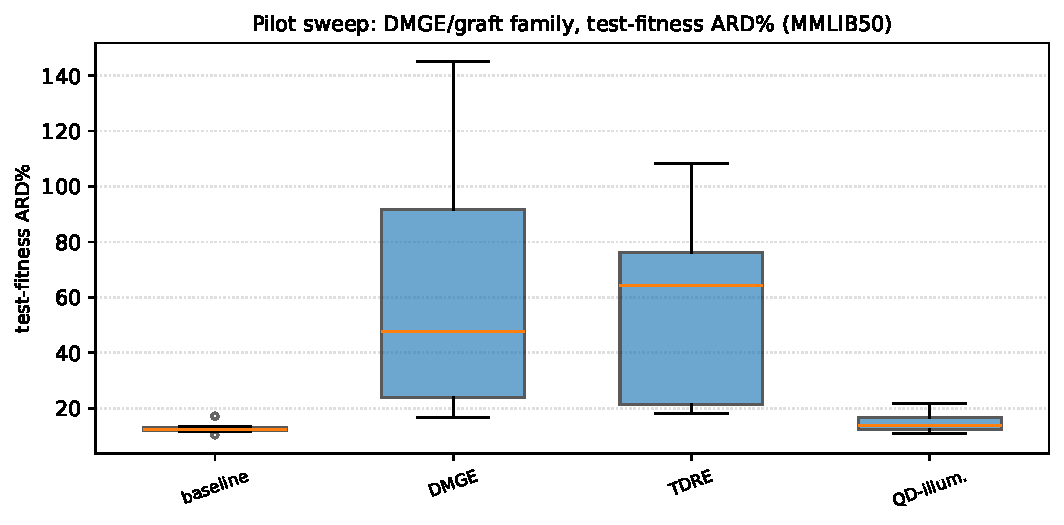
\includegraphics[width=0.85\textwidth]{img/generated/pilot_dmge_boxplot.pdf}
  \caption{Distribution of held-out test-fitness ARD\% across the three
  graft/trace-based variants and the baseline, 10 seeds per box. The two
  graft-based variants' boxes barely fit on the same axis as the
  baseline's, and their spread, not just their location, is the story:
  seed-to-seed standard deviations of 33--41 ARD\% points against the
  baseline's 1.7.}
  \label{fig:pilot-dmge-boxplot}
\end{figure}

\begin{figure}[htbp]
  \centering
  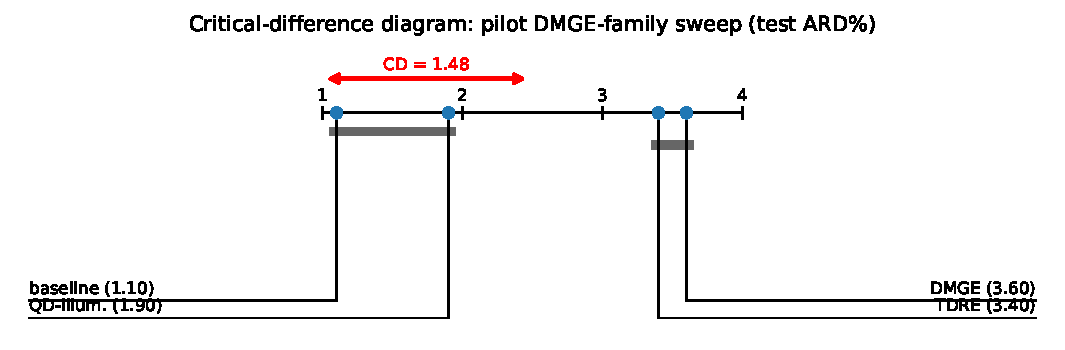
\includegraphics[width=0.85\textwidth]{img/generated/pilot_dmge_cd.pdf}
  \caption[Critical-difference diagram, pilot DMGE sweep]{Critical-difference
  diagram for the pilot DMGE-family \changed{comparison} (test ARD\%, Nemenyi CD at
  $\alpha=0.05$ for $k=4$ conditions and $N=10$ seed blocks). The baseline
  and the QD-illumination variant form one group, DMGE and TDRE a second,
  clearly separated one.}
  \label{fig:pilot-dmge-cd}
\end{figure}

The numbers in Table~\ref{tab:pilot-dmge-results}\changed{, visualised in
Figures~\ref{fig:pilot-dmge-boxplot} and~\ref{fig:pilot-dmge-cd},} turn the qualitative
verdict above into a quantitative one, and add a mechanism for the
``instability'' this section has so far described only informally. On the
common held-out test scale, DMGE and TDRE average 60.27 and 56.48 ARD\%
against the baseline's 12.74, worse in every single paired seed
($r=-1.000$), with seed-to-seed standard deviations twenty times the
baseline's; the QD-illumination variant, which grafts nothing and only
changes the archive structure, lands far closer (14.75) but still
significantly worse ($p=0.0176$). Part of the graft variants' collapse has
an identifiable cause that is itself instructive: their evolved rules lean
on the NR-dependent graft vocabulary, terminals that are only meaningful
on the NR-preserving instances they trained on and degrade to neutral
constants on the common test set, so entire grafted branches of the
evolved trees go inert at test time. A mechanism that conditions its
repairs on instance-set-specific terminals does not merely fail to help;
it produces rules that cannot survive a change of instance distribution.
An independent replication of \changed{the pilot comparison} on a disjoint seed set
reproduced this collapse in full (DMGE 38.05, TDRE 51.92 mean test ARD\%,
both still worse than the baseline in essentially every paired seed), so
the family's failure is a property of the mechanism, not of one draw of
seeds. \changed{None of the three variants justified the comprehensive
stage's cost, and none reappear in
Section~\ref{sec:operator-evaluation}.}

\changed{While DMGE did not provide the expected improvement, some of the
individual modifications were worth evaluating on their own. Modification
2's non-renewable-resource terminals are the clearest case: inside DMGE
their individual contribution could not be separated from the graft
mechanism's instability and cost. After the graft-based schemes were set
aside, these terminals were extended with a third, forward-looking one
(\texttt{NR\_BUDGET\_PRESSURE}, Section~\ref{subsec:nr-terminals-definition})
and evaluated as a strictly additive change to the terminal set, with no
grafting logic around them; they went on to become this thesis's strongest
result.}

\subsection{Exploratory investigation of enriched terminal sets}
\label{subsec:pilot-terminals}

DMGE's abandonment did not end the search for a variation- or
representation-side improvement; it redirected it. Immediately after the
pivot away from graft-based variation, three further terminal-set
extensions were tried in quick succession, each motivated directly by what
the previous one had (or had not) shown, which makes this round less a
grab-bag of ideas than a single chain of reasoning carried out in code.

\textbf{Critical-path propagation terminals.} The baseline already exposes
classic CPM dates (earliest/latest start and finish) as terminals, but
computes them once and leaves the GP tree to recombine them into anything
subtler, such as slack, itself. The first idea tried was to hand the GP a
more "ready-made" critical-path signal instead: four extra per-activity
features, computed once per instance and never recomputed during a run.
\changed{Writing $f(i) = d^{\min}_i + \max_{s \in S_i} f(s)$ for the
forward propagation score (the longest minimum-duration chain from $i$ to
the sink) and $b(i) = \min_{s \in S_i} b(s) - d^{\min}_i$ for its backward
counterpart, both normalised by the CPM makespan, the four terminals are
\begin{align*}
  \texttt{CP\_FORWARD} &= f(i), &
  \texttt{CP\_BACKWARD} &= b(i),\\
  \texttt{CP\_SLACK\_SCORE} &= b(i) - f(i), &
  \texttt{CP\_PROB} &= \frac{f_{\mathrm{raw}}(i)}{\max_{j} f_{\mathrm{raw}}(j)},
\end{align*}
the last being a criticality score relative to the most critical
activity.} At pilot scale (population 60, 25 generations, 5
MMLIB50 instances, 10 seeds), this sped up convergence noticeably (a mean
of 8.7 generations to reach the best solution, against 14.4 for the
baseline) and produced the single best individual run observed in this
round, but moved neither the mean training fitness nor the held-out test
fitness in any meaningful way \changed{(Table~\ref{tab:pilot-terminals-results})}. The diagnosis was
that one of the four new terminals is algebraically identical to the
existing LS terminal, and the other three are linear recombinations of
terminals the GP could already construct: the pilot rediscovered a shortcut
to something already reachable, not new information, which explains the
convergence-speed gain without a quality gain. This diagnosis is precisely
what motivated the next idea.

\textbf{Resource-constrained critical-path (RCCP) terminals.} If
precedence-only critical-path information was already redundant, the
natural next hypothesis was that \emph{resource-driven} criticality, which
no combination of the existing precedence-only terminals can express,
would fare better. Five terminals were added along these lines.
\changed{Let $k^{*}$ be the currently most contended (bottleneck)
renewable resource, i.e.\ the one maximising the utilisation
$u_k = 1 - \mathrm{avail}_k / R^{\rho}_k$, let $u^{*} = u_{k^{*}}$, and
let $E$ be the current eligible-activity set. The terminals are
\begin{align*}
  \texttt{RCCP\_BOTTLENECK\_UTIL} &= u^{*},\\
  \texttt{RCCP\_CANDIDATE\_CONTENTION} &=
    \frac{r^{\rho}_{jmk^{*}}}{\mathrm{avail}_{k^{*}}},\\
  \texttt{RCCP\_SLACK} &= \texttt{CP\_SLACK\_SCORE} \cdot (1 - u^{*}),\\
  \texttt{RCCP\_PRESSURE\_TREND} &=
    \frac{\sum_{i \in E} \min_{m} r^{\rho}_{imk^{*}}}{\mathrm{avail}_{k^{*}}},
\end{align*}
i.e.\ the bottleneck utilisation itself, the candidate mode's demand on
the bottleneck relative to what remains, a resource-discounted slack
score, and a forward-looking demand/remaining-supply ratio over the
currently eligible activities; the fifth,
\[
  \texttt{RCCP\_RESOURCE\_CONCENTRATION} =
  1 + \frac{\sum_{k \in \mathcal{R}^{\rho}} p_k \ln p_k}{\ln |\mathcal{R}^{\rho}|},
\]
where $p_k = r^{\rho}_{jmk} / \sum_{k'} r^{\rho}_{jmk'}$ is the share of
resource $k$ in the mode's total renewable demand, is one minus the normalised
Shannon entropy of the candidate mode's demand distribution over renewable
resource types, distinguishing a mode that draws heavily on one resource
type from one that spreads its demand thinly across several.} At
the same pilot scale (population 60, 25 generations, 5 MMLIB50 instances,
10 seeds, baseline / CP-propagation / RCCP / both combined), the result was
a second null: training fitness was statistically indistinguishable across
all four conditions \changed{(Table~\ref{tab:pilot-terminals-results})}.
Giving the GP live resource-contention information, not just
precedence information, did not translate into better trees at this scale
either\changed{, a second null result alongside
critical-path propagation}.

\textbf{Mode-interaction terminals.} A third, structurally different
hypothesis remained: rather than a \emph{budget} signal (how much of a
resource is left) or a \emph{contention} signal (who is competing for it
right now), a \emph{consequence} signal, how much choosing a given mode for
one activity narrows down the feasible mode choices left for other,
not-yet-scheduled activities sharing a resource window with it.
\changed{Three terminals implement this idea. Writing $E' = E \setminus
\{j\}$ for the other currently eligible activities and
$\mathrm{avail}_k$ for the current remaining capacity of renewable
resource $k$, and $\mathcal{K}_{jm} = \{\, k : r^{\rho}_{jmk} > 0 \,\}$
for the resource types the candidate mode actually uses. With
$\phi(i) = |\{\, m' \in \mathcal{M}_i : \exists k:\;
r^{\rho}_{im'k} > \mathrm{avail}_k - r^{\rho}_{jmk} \,\}|$ counting
neighbour $i$'s modes that committing the candidate mode would make
resource-infeasible:
\begin{align*}
  \texttt{MI\_CONSTRAINT\_TIGHTENING} &=
    \frac{1}{|E'|} \sum_{i \in E'} \frac{\phi(i)}{|\mathcal{M}_i|},\\
  \texttt{MI\_RECIPROCAL\_SCARCITY} &=
    \frac{|\{\, k \in \mathcal{K}_{jm} :
      \textstyle\sum_{i \in E'} \min_{m'} r^{\rho}_{im'k} > \mathrm{avail}_k \,\}|}
      {|\mathcal{K}_{jm}|},\\
  \texttt{MI\_ACTIVITY\_PRESSURE} &=
    \frac{1}{|\mathcal{M}_j|} \sum_{m \in \mathcal{M}_j}
    \texttt{MI\_CONSTRAINT\_TIGHTENING}(j, m),
\end{align*}
i.e.\ the average fraction of neighbours' modes the candidate mode would
make infeasible; a cheaper proxy counting
for how many of the candidate's resources the neighbours' combined
cheapest-mode demand already exceeds availability; and the first measure
averaged over the candidate activity's own modes (activity tree). These}
were the least literature-established of any extension
tried, by design: there is comparatively little precedent in the published
GPHH/RCPSP literature for a consequence-based terminal of this kind, so a
null result here was always going to be exactly as informative as a
positive one. It was, in fact, worse than null
\changed{(Table~\ref{tab:pilot-terminals-results})}: mode-interaction
terminals alone were not significant against baseline
\changed{(and the mean moved in the \emph{wrong} direction)}, and stacking
them with RCCP terminals made things actively worse, significantly so.
Combining two sets of additional
terminals compounded noise rather than information, a caution worth
carrying forward whenever new terminals are added to an already-rich
feature set.

\begin{table}[htbp]
  \centering
  \small
  \caption[Pilot results: enriched terminal sets]{\changed{Pilot results for
  the enriched-terminal-set round: mean training-fitness ARD\% (\%), 10
  seeds per condition, paired two-sided Wilcoxon $p$ against the matching
  baseline run. The two blocks are separate pilot runs, each compared
  against its own baseline.}}
  \label{tab:pilot-terminals-results}
  \begin{tabular}{lrr}
    \toprule
    \textbf{Condition} & \textbf{Train mean} & \textbf{$p$} \\
    \midrule
    Baseline                         & 12.25 & --    \\
    CP-propagation terminals         & 12.39 & 0.82  \\
    RCCP terminals                   & 12.55 & 0.46  \\
    CP-propagation + RCCP            & 12.25 & 1.00  \\
    \midrule
    Baseline (second run)            & 12.40 & --    \\
    Mode-interaction terminals       & 13.37 & 0.16  \\
    Mode-interaction + RCCP          & 14.21 & 0.04 \\
    \bottomrule
  \end{tabular}
\end{table}

Read together, this second exploratory round systematically worked through
precedence-based, resource-budget-based, resource-contention-based, and
consequence-based signals, in that order, each motivated by the previous
result's diagnosis, and none of the three terminal-set ideas tried here
justified carrying forward. Non-renewable resource terminals
(Section~\ref{subsec:nr-eval}) close a different, and as it turned out
genuinely open, information gap, visibility into non-renewable rather than
renewable resource state, which is precisely why they, and not any of the
three ideas in this subsection, were the one representation-side extension
promoted to the comprehensive stage.

\subsection{\texorpdfstring{\changed{Epsilon-lexicase selection and critical-path local search: staged evaluation}}{Epsilon-lexicase selection and critical-path local search: staged evaluation}}
\label{subsec:pilot-lexicase-iteration}

\changed{The third screened direction changed the search process rather
than the representation, combining two mechanisms. Tournament selection
was replaced by epsilon-lexicase selection (module \texttt{hybrid\_gp.py};
defined in full in Section~\ref{subsec:lexicase-definition}), motivated by
the fact that tournament selection on mean deviation collapses
per-instance scores into a single number and can converge prematurely onto
generalists, whereas lexicase treats every training instance as a separate
selection case and keeps specialists alive. On top of it, a memetic
local-search step was added (module \texttt{local\_search.py}; defined in
full in Section~\ref{subsec:localsearch-definition}) that runs a
critical-path repair, mode reassignment, precedence-respecting activity
swaps, and slack-based resource shifts, on the top $8\%$ of the population
every generation. The local search only ever overwrites an individual's
recorded fitness, never the GP tree itself, so the representation remains
exactly the baseline's (the Baldwinian design of
Section~\ref{subsec:localsearch-definition}). One supporting change was
needed: fitness evaluation (\texttt{evaluate\_heuristic} in
\texttt{gphh\_solver.py}) now also stores each individual's vector of
per-instance deviations (\texttt{case\_fitness}), which is what lexicase
selection filters on, case by case.}

\changed{This combination was evaluated in four stages of increasing scale
and cost, summarised in Tables~\ref{tab:lexicase-stages}
and~\ref{tab:lexicase-stages-consequences} and described below.}

\begin{table}[htbp]
  \centering
  \small
  \shrinktofit{%
  \caption[Escalating evidence for lexicase selection]{The four
  evidence-escalation stages of the lexicase follow-up, each on serial SGS
  against the tournament baseline (stage 1 measured the combination with
  the memetic local search; stages 2--4 measured lexicase in isolation).
  The training-fitness advantage strengthens with every escalation while
  the test-fitness effect, seemingly headed for significance at stages
  2--3, reverses at stage 4, the effect-size inflation episode discussed
  below.}
  \label{tab:lexicase-stages}
  \begin{tabular}{lll}
    \toprule
    \textbf{Stage} & \textbf{Scale} & \textbf{Outcome (lexicase vs.\ baseline)} \\
    \midrule
    1. First pass (with LS) &
    pop.\ 60, gen.\ 25, 5 inst., $n{=}10$ &
    train 11.87 vs.\ 13.48; $p{=}0.0059$, $r{=}0.93$ \\
    2. Official split &
    pop.\ 60, gen.\ 20, 10 classes, $n{=}10$ &
    \changed{train 16.58 vs.\ 18.05; $p{=}0.0098$, $r{=}0.89$; test 18.57 vs.\ 19.40; $p{=}0.109$} \\
    3. Power follow-up &
    stage 2 + 6 seeds ($n{=}16$) &
    \changed{train 16.57 vs.\ 17.91; $p{=}0.00058$, $r{=}0.90$; test 18.71 vs.\ 19.43; $p{=}0.074$, $r{=}0.543$} \\
    4. Extended follow-up &
    $n{=}31$ &
    \changed{train 16.68 vs.\ 17.60; $p{=}0.0002$, $r{=}0.72$; test 18.93 vs.\ 19.22; $p{=}0.325$, $r{=}0.209$} \\
    \bottomrule
  \end{tabular}%
  }
\end{table}

\begin{table}[htbp]
  \centering
  \small
  \shrinktofit{%
  \caption[Consequences of the lexicase iteration]{The two follow-on
  decisions the iteration produced: a gap-aware early-stopping mechanism
  built to act on the train/test asymmetry, which failed both validations
  and was retired, and the $2 \times 2$ ablation design (baseline,
  lexicase alone, local search alone, combined) that was promoted wholesale
  into the comprehensive stage rather than re-run at pilot scale.}
  \label{tab:lexicase-stages-consequences}
  \begin{tabular}{lll}
    \toprule
    \textbf{Follow-on} & \textbf{Design} & \textbf{Outcome} \\
    \midrule
    Gap-aware stopping &
    two validations, $n{=}10$ &
    n.s.\ ($p{=}0.109$ / $p{=}0.734$); retired \\
    $2 \times 2$ ablation &
    pop.\ 1\,000, gen.\ 50, $n{=}30$, full grid &
    became Chapter~\ref{chap:experiments}'s condition set \\
    \bottomrule
  \end{tabular}%
  }
\end{table}

The first pilot pass (population 60, 25 generations, 5 MMLIB50 instances,
10 seeds) combined epsilon-lexicase selection with \changed{the
critical-path local search (a hill-climbing refinement of elite
individuals' schedules, defined in
Section~\ref{subsec:localsearch-definition})} and found a large,
significant effect: mean training fitness of 11.87 against the baseline's
13.48, best-of-run 10.07 against 12.35, Wilcoxon $p=0.0059$ with a large
rank-biserial effect size ($r=0.93$). Convergence was slower under lexicase
(17.5 generations to best solution, against 12.0 for the baseline), which
is exactly what a case-by-case, diversity-preserving selection pressure
would be expected to do relative to tournament selection's tendency to
collapse onto a single strong generaliser early.

A second, larger pass moved to the official 60/20/20 train/validation/test
split on real MMLIB50, stratified down to 10 of the 108 classes because the
literal paper specification (population 1\,000, 50 generations, the full
class split) would have taken an estimated 200-plus days on the hardware
available at that stage (population 60, 20 generations, 10 seeds, both
serial and parallel SGS, three conditions: baseline, lexicase, lexicase
with local search). \changedB{The same 10-class stratification was later
retained for the comprehensive stage as well
(Section~\ref{subsec:instance-sampling}): \emph{training} on the full
108-class split was never computationally within reach at the paper's own
budget, since the training set sits inside the GP loop and its cost is
paid again for every individual in every generation. Testing carries no
such multiplier, so the rules evolved at the comprehensive stage are
additionally re-evaluated, after evolution, on the complete 108-class
held-out test set (Section~\ref{subsec:full108}).} On serial SGS, both
lexicase and the full combination significantly beat the baseline on
training fitness ($p=0.0098$ and $p=0.027$); the same comparison on
held-out test fitness landed at $p=0.109$ for lexicase, same direction, not
yet under the conventional 0.05 threshold. This pass also surfaced an
unplanned finding that turned out to matter more, at this scale, than the
selection mechanism under study: serial SGS dramatically outperformed
parallel SGS for every condition (test fitness around 18--19 versus 30--33),
a scale-of-effect difference between decoding schemes that later motivated
reporting every comprehensive-stage result broken down by SGS rather than
pooled across it (Section~\ref{sec:operator-evaluation}).

A quick power calculation on the $p=0.109$, $n=10$ result (effect size
$r=0.667$) suggested that 14--16 seeds might be enough to reach
significance, so six more seeds were added to that one comparison alone
rather than re-running the full grid. \changed{Two methodological caveats
apply to this step. First, adding observations
until a test reaches significance is a form of sequential testing without
correction, which inflates the false-positive rate; had the extension
produced $p<0.05$, that value could not have been taken at face value.
Second, the power calculation itself was built on a single small-sample
effect-size estimate. Both caveats turned out to matter, in the
conservative direction:} at $n=16$, the result moved to
$p=0.074$ ($r=0.543$), still short of significance, while training fitness,
already significant at $n=10$, became more so ($p=0.00058$)\changed{, and
extending the same comparison to $n=31$ \emph{weakened} the test-fitness
effect, to $p=0.325$ and $r=0.209$, instead of strengthening it.} The
$n=10$ estimate of $r=0.667$ had been small-sample
noise, not an early signal of a real, strengthening trend, a textbook
instance of effect-size inflation from an underpowered pilot. Training
fitness, meanwhile, stayed exactly where the larger samples had already
placed it: significant, and increasingly so ($p=0.0002$, $r=0.72$,
mean 16.68 for lexicase against 17.60 for baseline). \changed{The reading
at this scale was that lexicase selection reliably fits the training
instances better, but that advantage was not showing up as significantly
better generalisation. Partly in response to this episode, every
comprehensive-stage comparison in
Section~\ref{sec:operator-evaluation} was planned at a fixed $n=30$
decided in advance, not adaptively in response to interim $p$-values.}

\changed{Despite the $n=31$ null on test fitness, lexicase remained
interesting enough to carry into the comprehensive stage: its
training-fitness advantage was the most consistent positive signal any
screened mechanism had produced, the null covered only one decision
strategy and one decoding scheme at a reduced budget, and evaluating
lexicase added little extra cost to a comprehensive experiment whose
baseline runs had to be executed in any case. The comprehensive stage then
confirmed the train/test asymmetry across the full grid and, on MMLIB100,
found that it widens rather than resolves
(Section~\ref{subsec:lexicase-eval}).}

\changed{One design decision followed directly from this iteration: a full
$2 \times 2$ ablation, baseline, lexicase alone, local search alone, and
the two combined, became the core of the comprehensive stage's
experimental design (the conditions \texttt{baseline}, \texttt{lexicase},
\texttt{local\_search} and \texttt{hybrid} of
Chapter~\ref{chap:experiments}). The ablation was needed because every
pilot result up to the second pass had measured lexicase either in
combination with the local search or alongside it, so the two mechanisms'
individual contributions could not be separated: a gain or loss observed
for the combination could belong to either component, or to their
interaction. Running all four conditions at full statistical power is what
later made it possible to show that the combination underperforms both of
its own components (Section~\ref{subsec:final-comparison}).}

One further side-investigation grew directly out of this asymmetry and
also ended in a null result. Examining per-seed
training/validation fitness trajectories suggested that lexicase's
train/validation gap stays flat for several generations and then widens
onto a stable, higher plateau, with none of the later training-fitness
gains transferring to held-out data. A gap-onset detector was built to
catch this transition from the run's own validation trajectory (not a
hard-coded generation) and used to roll back to the best-on-validation
generation's individual, or stop the run early, once onset was detected.
Validated twice, once at a scale with no real train/test gap to catch (so
inconclusive by construction) and once against a known-gap 10-class split,
the detector correctly identified the onset generation and rolled back in
8--9 of 10 seeds, to a mean generation roughly a third to half of the full
budget, but gap-aware early stopping was never significantly better than
plain lexicase on test fitness ($p=0.109$ and $p=0.734$ in the two
validations), and the generalisation gap itself barely moved. The diagnosis was that
validation-set ``best so far'' is too noisy an estimator, at only 10--25
held-out instances, to reliably identify the generation that will actually
generalise best to a third, fully held-out set: the gap is real, but this
particular way of acting on it was not precise enough to help. This
mechanism was retired after that result and is not part of the
lexicase condition evaluated in Section~\ref{subsec:lexicase-eval}.

\changed{The methodological lesson of this iteration is that an early
effect-size estimate from a small pilot, even one that looks clean and
significant, should be treated as a hypothesis about direction, not
magnitude: a follow-up power calculation built on one such estimate can
point the wrong way once more data arrives.}

\changed{Table~\ref{tab:screening-verdicts} summarises the verdict on
every screened direction: only epsilon-lexicase selection, critical-path
local search and the non-renewable resource terminals were carried
forward into the comprehensive evaluation.}

\begin{table}[htbp]
  \centering
  \small
  \shrinktofit{%
  \caption[Screening verdicts]{\changed{Summary of the exploratory
  screening: the verdict on every screened direction and where its
  evidence is reported.}}
  \label{tab:screening-verdicts}
  \begin{tabular}{lll}
    \toprule
    \textbf{Screened direction} & \textbf{Pilot outcome} & \textbf{Decision} \\
    \midrule
    DMGE / TDRE / QD illum.    & significantly worse (Table~\ref{tab:pilot-dmge-results}) & dropped \\
    CP-prop.\ / RCCP / MI terminals & null or worse (Table~\ref{tab:pilot-terminals-results}) & dropped \\
    Epsilon-lexicase selection & consistent training-fitness wins (Table~\ref{tab:lexicase-stages}) & carried forward \\
    Critical-path local search & positive first pass with lexicase (Table~\ref{tab:lexicase-stages}) & carried forward \\
    NR resource terminals      & extracted from DMGE toolkit (Section~\ref{subsec:pilot-dmge}) & carried forward \\
    \bottomrule
  \end{tabular}%
  }
\end{table}


\chapter{Experimentation and comparison}
\label{chap:experiments}

Chapter~\ref{chap:approach} proposed a genetic-programming hyper-heuristic
(GPHH) baseline and a family of candidate modifications to it. This chapter
reports how those candidates were actually evaluated, and, just as
importantly, how the space of candidates was narrowed before any of them
was evaluated at full scale. The experimental programme underlying this
chapter was carried out in two clearly separated stages. An
\emph{exploratory} stage (Section~\ref{sec:parameter-sensitivity}) screened
a wide range of algorithmic ideas cheaply, using small populations, few
generations and few benchmark instances, with the explicit purpose of
generating and discarding hypotheses rather than producing publishable
numbers. A \emph{comprehensive} stage (Section~\ref{sec:operator-evaluation})
then took the small number of ideas that survived screening and evaluated
them at the scale, statistical power and instance coverage required to
support a scientific claim. Rather than evaluating every idea exhaustively,
preliminary experiments were first used to identify promising research
directions, and only those directions were carried forward into the
expensive, fully powered study. \changed{Two terms are used with a fixed
meaning throughout this chapter: a \emph{condition} is one algorithm
configuration under comparison (the baseline, or the baseline with one
proposed modification applied), and a \emph{cell} is one combination of
schedule generation scheme and GP decision strategy; every condition is
evaluated in every cell, on both benchmark datasets, with 30 random seeds
each.}

\section{Software implementation}
\label{sec:software-implementation}

All experiments were run against a single, shared code base
(\texttt{GP\_MRCPSP\_CEC2024/yuantian}) built on top of Tian, Mei and
Zhang's own reference implementation~\cite{Tian2024GPHH}, using
DEAP~\cite{derainville2012deap} for the underlying evolutionary loop
(population handling, crossover, mutation, and the tree representation
itself) and the \texttt{discrete-optimization} library for canonical
schedule decoding and feasibility checking. Every configuration compared in
this chapter, baseline and every proposed modification alike, therefore
shares the same GP engine, the same multi-tree individual representation
(Section~\ref{subsec:individual-representation}), the same instance parser,
and the same fitness computation; configurations differ only in the
specific, additive change under test (selection operator, elite refinement
step, or terminal set), so that a difference in outcome can be attributed
to that change rather than to incidental implementation drift between
otherwise-unrelated codebases.

The exploratory and comprehensive stages are implemented as two separate,
purpose-built harnesses within this shared code base. \changed{For clarity
of attribution: the \texttt{yuantian/} directory vendors \changedC{Tian,
Mei and Zhang's reference implementation~\cite{Tian2024GPHH}}, and everything evaluated in this chapter beyond
the plain baseline, the \texttt{exploratory/} and \texttt{experiments/}
modules and every extension condition, is this thesis's own addition
inside that directory, kept there so that the extensions and the reference
implementation share one code and import structure.}
\changed{Section~\ref{sec:parameter-sensitivity}'s pilot experiments are driven by
\texttt{yuantian/exploratory/} (one module per screened mechanism): the
DMGE-family comparison via
\texttt{yuantian/experiments/exploratory\_sweep\_experiment.py}, and the
staged lexicase/local-search evaluation via
\texttt{lexicase\_local\_search\_experiment.py} and
\texttt{full\_mmlib\_experiment.py}.}
Section~\ref{sec:operator-evaluation}'s comprehensive evaluation is driven
by a single \emph{matrix} experiment,
\texttt{yuantian/experiments/matrix\_runner.py}, parameterised by condition
(baseline, lexicase, local search, hybrid, NR terminals, and NR terminals'
own matched control), GP decision strategy (activity-first, mode-first,
simultaneous), schedule generation scheme (serial, parallel), benchmark
dataset, and random seed; \texttt{matrix\_config.py} is the single source
of truth for this grid and for the fixed parameter values reported in
Table~\ref{tab:experimental-parameters}. Because the full grid at the
paper's own population and generation budget is computationally heavy, runs
were distributed as PBS array jobs on the MetaCentrum computing grid
(Section~\ref{subsec:hw-sw}), and results were aggregated and tested for
significance offline with \texttt{yuantian/experiments/analyze\_matrix.py}
and \texttt{final\_comparison\_report.py}, which implement the statistical
methodology of Section~\ref{subsec:statistical-methodology} uniformly
across every condition and dataset.

\section{Experimental setup}
\label{sec:experimental-setup}

This section fixes the experimental protocol used throughout the rest of
the chapter: the hardware and software environment, the benchmark
instances and how they were sampled, the algorithm's parameters, the number
of independent runs, the evaluation metric, and the statistical procedure
used to decide whether an observed difference is meaningful. The same
protocol is used, without modification, for the exploratory and the
comprehensive stage; only the scale (population size, generation count,
instance count, and seed count) differs between them, as detailed in each
stage's own section.

\subsection{Hardware and software environment}
\label{subsec:hw-sw}

\changed{All runs were executed on the MetaCentrum national computing
grid. Table~\ref{tab:hw-sw-config} summarises the software environment,
the per-job resource allocation, and how jobs were scheduled.}

\begin{table}[htbp]
  \centering
  \small
  \caption[Hardware and software configuration]{\changed{Hardware and
  software configuration used for the runs reported in this chapter.
  Individual jobs were placed by the PBS scheduler on whichever grid nodes
  were available, so the exact hardware varies from run to run; the
  submission environment and per-job resource allocation below were
  constant.}}
  \label{tab:hw-sw-config}
  \begin{tabular}{@{}p{0.27\textwidth}p{0.65\textwidth}@{}}
    \toprule
    \textbf{Component} & \textbf{Configuration} \\
    \midrule
    Compute platform & MetaCentrum national computing grid (OpenPBS scheduler, version 23.06.06) \\
    \changed{Submission host} & \changed{\texttt{tarkil.grid.cesnet.cz}; compute nodes assigned per job by the scheduler (heterogeneous hardware)} \\
    Per-job allocation & 1 node, 8 CPU cores, 8\,GB RAM, 8\,GB local scratch \\
    Parallelism & population evaluation parallelised across 8 cores per run (\texttt{--multiprocess}) \\
    \changed{Operating system} & \changed{Debian GNU/Linux 12 (``bookworm'') on the submission host; node OS varies with the assigned machine} \\
    Python & 3.11.2, loaded via module \texttt{python/\allowbreak3.11.11-\allowbreak gcc-\allowbreak 10.2.1-\allowbreak 555dlyc} \\
    Core libraries & DEAP~\cite{derainville2012deap}, \texttt{discrete-optimization}, NumPy 1.24.2, SciPy \\
    Job scheduling & one PBS array element per (condition, strategy, SGS, dataset, seed) combination \\
    \bottomrule
  \end{tabular}
\end{table}

\subsection{Benchmark datasets and instance sampling}
\label{subsec:instance-sampling}

Both the exploratory and the comprehensive stage draw instances from
MMLIB50 and MMLIB100 (Section~\ref{subsec:mmlib}). \changed{Each MMLIB
dataset consists of 108 instance classes of five instances each, where a
class is one combination of the generator's OS/RF/RS target levels
(Section~\ref{subsec:indicators}). Following Tian et al.'s 60/20/20
convention, the five instances of every class are split into three
training instances, one validation instance and one test instance, so a
run trained on $n_{\text{classes}}$ classes sees $3\,n_{\text{classes}}$
training instances and is tested on $n_{\text{classes}}$ held-out ones.
\changed{The training, validation and test instances of a class therefore
always share the same OS/RF/RS setting: generalisation is measured to
\emph{unseen instances with the same characteristics}, not to unseen
characteristics.}
All planned runs of the comprehensive stage were completed, but on a
stratified subset of $n_{\text{classes}}=10$ classes, evenly spaced across
each dataset's class-index range (class indices $1, 11, 21, \dots, 91$)
and identical for every condition and
every seed, so that the subsampling cannot bias the comparison between
conditions. Because MMLIB numbers its classes systematically along the
generator's OS/RF/RS parameter grid, an even stride over the class indices
samples across the whole range of instance characteristics rather than
clustering in one region (the selected classes cover
$\mathrm{OS} \in \{0.25, 0.5, 0.75\}$, $\mathrm{RF} \in \{0.5, 1.0\}$
and RS from tight to effectively unconstrained,
cf.\ Table~\ref{tab:per-class-breakdown}); \changedC{it is, however, a
deterministic stride and does not guarantee that every OS/RF/RS
combination receives a class, so some parameter combinations are
unrepresented;} evaluating on all 108 classes at the paper's population and
generation budget would have required an estimated several hundred days of
computation\changedC{, which could not have been completed within the time
frame of this thesis}.}
Table~\ref{tab:experimental-parameters}
records this together with the remaining fixed settings.

\subsection{Algorithm parameters}
\label{subsec:algorithm-parameters}

\changed{Table~\ref{tab:experimental-parameters} lists the fixed parameter
values used throughout the comprehensive stage; except for the reduced
class count $n_{\text{classes}}$, they match the configuration of Tian et
al.~\cite{Tian2024GPHH}.}

\begin{table}[htbp]
  \centering
  \small
  \caption[Experimental parameters]{Fixed parameter values used throughout
  the comprehensive evaluation stage (Section~\ref{sec:operator-evaluation}).
  These match Tian et al.'s~\cite{Tian2024GPHH} own reported configuration
  except for $n_{\text{classes}}$, which is reduced from the paper's full
  108-class split for computational tractability
  (Section~\ref{subsec:instance-sampling}); the exploratory stage
  (Section~\ref{sec:parameter-sensitivity}) instead uses a substantially
  smaller population, generation count and instance count, since its purpose
  is cheap screening rather than a publishable estimate.}
  \label{tab:experimental-parameters}
  \begin{tabular}{@{}p{0.55\textwidth}p{0.35\textwidth}@{}}
    \toprule
    \textbf{Parameter} & \textbf{Value} \\
    \midrule
    Population size & 1\,000 \\
    Generations & 50 \\
    Elite individuals carried forward & 10 \\
    Tournament size (baseline selection) & 7 \\
    Crossover rate / mutation rate & 0.80 / 0.15 \\
    Maximum tree depth & 8 \\
    Initial tree depth range (ramped half-and-half) & 2--6 \\
    Local search elite fraction / iterations & 8\% pop.\ / 10 iterations \\
    Stratified classes per dataset ($n_{\text{classes}}$) & 10 (of 108) \\
    Train / validation / test cases per class & 3 / 1 / 1 \\
    Independent seeds per configuration & 30 \\
    Seed range (comprehensive stage) & 12\,000--12\,029 \\
    \bottomrule
  \end{tabular}
\end{table}

\subsection{Independent runs and evaluation metric}
\label{subsec:runs-and-metric}

Every reported configuration (a condition, GP decision strategy and
schedule generation scheme combination) is repeated for 30 independent
random seeds in the comprehensive stage, matching the seed count used by
Tian et al.\ for Tables V and VI of the source paper and giving each
comparison a paired sample of 30 observations. The evaluation metric
throughout is the Average Relative Deviation (ARD\%) from the CPM lower
bound, defined in Section~\ref{sec:eval-metrics}; both the training-set ARD\%
(the quantity the GP search directly minimises) and the held-out test-set
ARD\% (the quantity that actually matters for generalisation) are reported
side by side wherever the two diverge in an interesting way, since a method
that only improves training fitness is not, on its own, evidence of a
better learned heuristic.

\subsection{Statistical methodology}
\label{subsec:statistical-methodology}

\changed{Table~\ref{tab:statistical-methodology} summarises the statistical
procedures applied uniformly to every comparison in this chapter; the
paragraphs below define them in detail.}

\begin{table}[htbp]
  \centering
  \small
  \caption[Statistical methodology]{Statistical procedures applied uniformly
  to every comparison in this chapter.}
  \label{tab:statistical-methodology}
  \begin{tabular}{@{}p{0.32\textwidth}p{0.58\textwidth}@{}}
    \toprule
    \textbf{Aspect} & \textbf{Procedure} \\
    \midrule
    Paired comparison (condition vs.\ baseline) & Wilcoxon signed-rank test, two-sided, $\alpha = 0.05$ \\
    Pairing unit & random seed (same stratified instance split across conditions) \\
    Effect size & matched rank-biserial correlation $r \in [-1, 1]$ \\
    Feasibility handling & per-instance feasible-only mean; a seed is dropped only if \emph{zero} instances were feasible under it (Section~\ref{sec:eval-metrics}) \\
    Multi-condition ranking & Friedman test across (SGS, decision strategy) cells as blocks, with average rank per condition, visualised as a critical-difference diagram \\
    Multiple comparisons & \emph{not} corrected for family-wise error across cells (Section~\ref{subsec:threats-stat}) \\
    \bottomrule
  \end{tabular}
\end{table}

Two comparisons recur throughout this chapter and are always reported
together: a \emph{pairwise} test (a candidate condition against its
baseline, one SGS/strategy cell at a time) and, where three or more
conditions are compared jointly (Section~\ref{subsec:final-comparison}), a
\emph{joint ranking} across cells. For the pairwise case, each cell's 30
seeds give 30 paired (baseline, condition) observations; a Wilcoxon
signed-rank test on these pairs is reported together with the matched
rank-biserial effect size $r$, which is signed so that $r>0$ means the
candidate condition achieved lower (better) ARD\% than baseline and $r<0$
means the opposite. For the joint-ranking case, each of the six (SGS,
strategy) cells contributes one observation per condition (that cell's mean
ARD\% under that condition), conditions are ranked 1 (best) to $k$ (worst)
within each cell, and a Friedman test on these ranks (blocks = cells)
checks whether the average ranks differ by more than chance.

\textbf{Boxplots.} Where referenced below, a boxplot shows the distribution
of a metric (typically test-set ARD\%) across the 30 seeds of a given
configuration: the box spans the interquartile range, the line inside it
is the median, whiskers extend to the most extreme non-outlier
observations, and individual points beyond the whiskers are plotted as
outliers. Boxplots are the primary way this chapter communicates
\emph{spread}, not just the mean reported in text: two configurations with
identical means but very different spreads represent a materially
different practical proposition (a consistently mediocre method versus an
unreliable but occasionally excellent one), and the mean/std pairs in the
descriptive-statistics tables alone can obscure that distinction.

\textbf{Critical-difference (CD) diagrams.} Where referenced below, a
critical-difference diagram plots each condition's average rank (as defined
above) on a shared axis and draws a bold horizontal bar connecting any
group of conditions whose average ranks are \emph{not} statistically
distinguishable at the chosen significance level, following the
convention popularised for classifier comparison by
Dem\v{s}ar~\cite{demsar2006}. A CD diagram
is reported only where the corresponding Friedman test is itself
significant; where it is not, the ranking is reported as a plain table
instead, since drawing a CD diagram over ranks that a Friedman test could
not distinguish from chance would visually overstate the evidence for a
difference between individual conditions' averaged ranks. \changed{Note
that the joint ranking has only the six (SGS, strategy) cells available as
blocks, which limits the resolution of the Friedman test and makes the
critical difference wide; this limitation is discussed together with the
other statistical caveats in the conclusion.}

\subsection{Reproducibility}
\label{subsec:reproducibility}

Every result file records enough information to be regenerated
independently: which of \texttt{matrix\_config.py}'s (condition, strategy,
SGS, dataset) cells it belongs to, the exact random seed, and per-instance
feasibility and fitness records for both the training and the held-out test
set. PBS array jobs read one row per array index from a checked-in
manifest CSV (\texttt{pbs\_jobs/*.manifest.csv}), so any individual cell can
be re-submitted in isolation; a completed result already present at the
persistent output location is not recomputed. \changed{One practical note
for re-running: the experiment scripts should be executed with
\texttt{python -O}, since the parallel simulator contains
\texttt{\_\_debug\_\_}-guarded diagnostic printing that otherwise floods
the logs.} The analysis scripts
(Section~\ref{sec:software-implementation}) are themselves committed to the
repository, so the numbers reported in
Sections~\ref{sec:operator-evaluation} and~\ref{sec:benchmark-comparison}
can be regenerated from the raw per-seed result files without re-running any
GP search. \changed{The exact version of the codebase used to produce all
results reported in this chapter, including the raw per-seed result files
themselves, is archived under the git tag \texttt{thesis-results} (commit
\texttt{a817f90}) and is publicly available at
\changedC{\url{https://github.com/sabinasagova/master-thesis/releases/tag/thesis-results}}.}

\section{Operator and local search evaluation}
\label{sec:operator-evaluation}

The pilot phase of Section~\ref{sec:parameter-sensitivity} narrowed a wide
field of candidate modifications down to three that were judged worth a
full, fully powered evaluation: epsilon-lexicase selection
(Section~\ref{subsec:lexicase-eval}), a critical-path-guided \changed{Baldwinian}
local search applied to elite individuals
(Section~\ref{subsec:localsearch-eval}), and a set of terminals exposing
non-renewable resource state to the GP
(Section~\ref{subsec:nr-eval}). Each is now compared against its matched
baseline at the full protocol of Section~\ref{sec:experimental-setup}: 30
seeds, population 1\,000, 50 generations, \changed{all three GP decision
strategies (activity-first, mode-first, simultaneous\changedC{, defined in
Section~\ref{subsec:individual-representation}}) and both schedule
generation schemes (serial and parallel\changedC{,
Section~\ref{subsec:sgs}}).}

This evaluation is run at full scale on \emph{both} benchmark sets, which
play complementary roles. \textbf{MMLIB50 is this thesis's primary evidence
base}: \changed{the full experiment grid, 6 conditions (baseline, lexicase,
local search, hybrid, NR terminals, and NR terminals' matched control
\texttt{baseline\_nr}) $\times$ 3 decision strategies $\times$ 2 schedule
generation schemes $\times$ 30 seeds $= 1\,080$ runs, is complete} and is
what each subsection's main
discussion is built on. \textbf{MMLIB100 is this thesis's scalability
validation at the same full scale}: doubling the number of activities per
instance roughly doubles the size of the precedence graph and the
combinatorial mode-assignment space the GP rule has to generalise over, so
\changed{MMLIB100 is where this thesis checks whether the MMLIB50 findings
are properties of the underlying mechanisms or artefacts of MMLIB50's
specific instance scale.} MMLIB100's grid is likewise complete (1\,080 of 1\,080
runs). Every subsection below therefore reports MMLIB100's real numbers
directly alongside MMLIB50's, under its own ``Scalability validation''
heading, with generated boxplots and, where the underlying Friedman test is
significant, critical-difference diagrams for both benchmark sets. In every
comparison table, a direction marker next to a condition's mean summarises
its change against the matched baseline in the same row:
\ArrBetter{} marks lower (better) ARD\%, \ArrWorse{} marks higher (worse)
ARD\%, and \ArrSame{} marks a mean equal to the baseline's at the reported
precision.

\subsection{Comprehensive evaluation of lexicase selection}
\label{subsec:lexicase-eval}

Epsilon-lexicase selection (defined in full in
Section~\ref{subsec:lexicase-definition}) is evaluated here, unchanged,
against the baseline at full statistical power; nothing else about the
algorithm changes, the representation, variation operators, and fitness
function are exactly as described in Chapter~\ref{chap:approach}.

\begin{table}[htbp]
  \centering
  \small
  \shrinktofit{%
  \caption[Lexicase vs.\ baseline on MMLIB50]{Mean ARD\% (\%), baseline vs.\
  epsilon-lexicase selection, MMLIB50, $n=30$ seeds per cell.}
  \label{tab:lexicase-vs-baseline-mmlib50}
  \begin{tabular}{llrrrr}
    \toprule
    \textbf{SGS} & \textbf{Strategy} & \textbf{Baseline (test)} & \textbf{Lexicase (test)} & \textbf{Baseline (train)} & \textbf{Lexicase (train)} \\
    \midrule
    Parallel & AF & 35.77 & 34.36\,\ArrBetter & 15.94 & 16.32\,\ArrWorse \\
    Parallel & MF & 35.78 & 35.50\,\ArrBetter & 16.61 & 16.98\,\ArrWorse \\
    Parallel & S  & 30.43 & 30.08\,\ArrBetter & 14.20 & 14.35\,\ArrWorse \\
    Serial   & AF & 17.81 & 18.33\,\ArrWorse &  9.83 &  9.64\,\ArrBetter \\
    Serial   & MF & 17.89 & 18.52\,\ArrWorse &  9.82 &  9.69\,\ArrBetter \\
    Serial   & S  & 18.08 & 18.41\,\ArrWorse & 10.29 &  9.92\,\ArrBetter \\
    \bottomrule
  \end{tabular}%
  }
\end{table}

\begin{table}[htbp]
  \centering
  \small
  \shrinktofit{%
  \caption[Descriptive statistics: lexicase vs.\ baseline]{Standard
  deviation and feasibility rate accompanying
  Table~\ref{tab:lexicase-vs-baseline-mmlib50}. Every seed produced
  feasible schedules under both conditions (feasibility rate 1.00
  throughout), so, unlike the NR terminals comparison
  (Section~\ref{subsec:nr-eval}), feasibility is not a differentiating
  factor here.}
  \label{tab:lexicase-descriptive-stats}
  \begin{tabular}{lllrrrr}
    \toprule
    \textbf{SGS} & \textbf{Strategy} & \textbf{Split} & \textbf{Baseline std} & \textbf{Lexicase std} & \textbf{Baseline feas.} & \textbf{Lexicase feas.} \\
    \midrule
    Parallel & AF & Train & 0.58 & 0.52 & 1.00 & 1.00 \\
    Parallel & AF & Test  & 2.74 & 3.22 & 1.00 & 1.00 \\
    Parallel & MF & Train & 0.66 & 0.55 & 1.00 & 1.00 \\
    Parallel & MF & Test  & 2.77 & 2.18 & 1.00 & 1.00 \\
    Parallel & S  & Train & 0.64 & 0.56 & 1.00 & 1.00 \\
    Parallel & S  & Test  & 2.24 & 1.95 & 1.00 & 1.00 \\
    Serial   & AF & Train & 0.25 & 0.19 & 1.00 & 1.00 \\
    Serial   & AF & Test  & 0.91 & 1.01 & 1.00 & 1.00 \\
    Serial   & MF & Train & 0.26 & 0.24 & 1.00 & 1.00 \\
    Serial   & MF & Test  & 0.91 & 0.92 & 1.00 & 1.00 \\
    Serial   & S  & Train & 0.24 & 0.20 & 1.00 & 1.00 \\
    Serial   & S  & Test  & 1.51 & 1.06 & 1.00 & 1.00 \\
    \bottomrule
  \end{tabular}%
  }
\end{table}

\begin{table}[htbp]
  \centering
  \small
  \shrinktofit{%
  \caption[Statistical significance: lexicase vs.\ baseline]{Two-sided
  paired Wilcoxon signed-rank test and matched rank-biserial effect size
  $r$ (positive favours lexicase, negative favours baseline), lexicase vs.\
  baseline, MMLIB50, $n=30$ per cell.}
  \label{tab:lexicase-significance}
  \begin{tabular}{lllrrl}
    \toprule
    \textbf{SGS} & \textbf{Strategy} & \textbf{Split} & \textbf{$p$} & \textbf{$r$} & \textbf{Verdict} \\
    \midrule
    Parallel & AF & Train & 0.0113 & $-0.523$ & Significant, favours baseline \\
    Parallel & AF & Test  & 0.1241 & $+0.325$ & Not significant \\
    Parallel & MF & Train & 0.0327 & $-0.445$ & Significant, favours baseline \\
    Parallel & MF & Test  & 0.6263 & $+0.105$ & Not significant \\
    Parallel & S  & Train & 0.3599 & $-0.196$ & Not significant \\
    Parallel & S  & Test  & 0.4771 & $+0.153$ & Not significant \\
    Serial   & AF & Train & 0.0030 & $+0.604$ & Significant, favours lexicase \\
    Serial   & AF & Test  & 0.0879 & $-0.359$ & Not significant \\
    Serial   & MF & Train & 0.0248 & $+0.467$ & Significant, favours lexicase \\
    Serial   & MF & Test  & 0.0252 & $-0.476$ & Significant, favours baseline \\
    Serial   & S  & Train & 0.0000 & $+0.888$ & Significant, favours lexicase \\
    Serial   & S  & Test  & 0.0519 & $-0.406$ & Not significant (borderline) \\
    \bottomrule
  \end{tabular}%
  }
\end{table}

\begin{figure}[htbp]
  \centering
  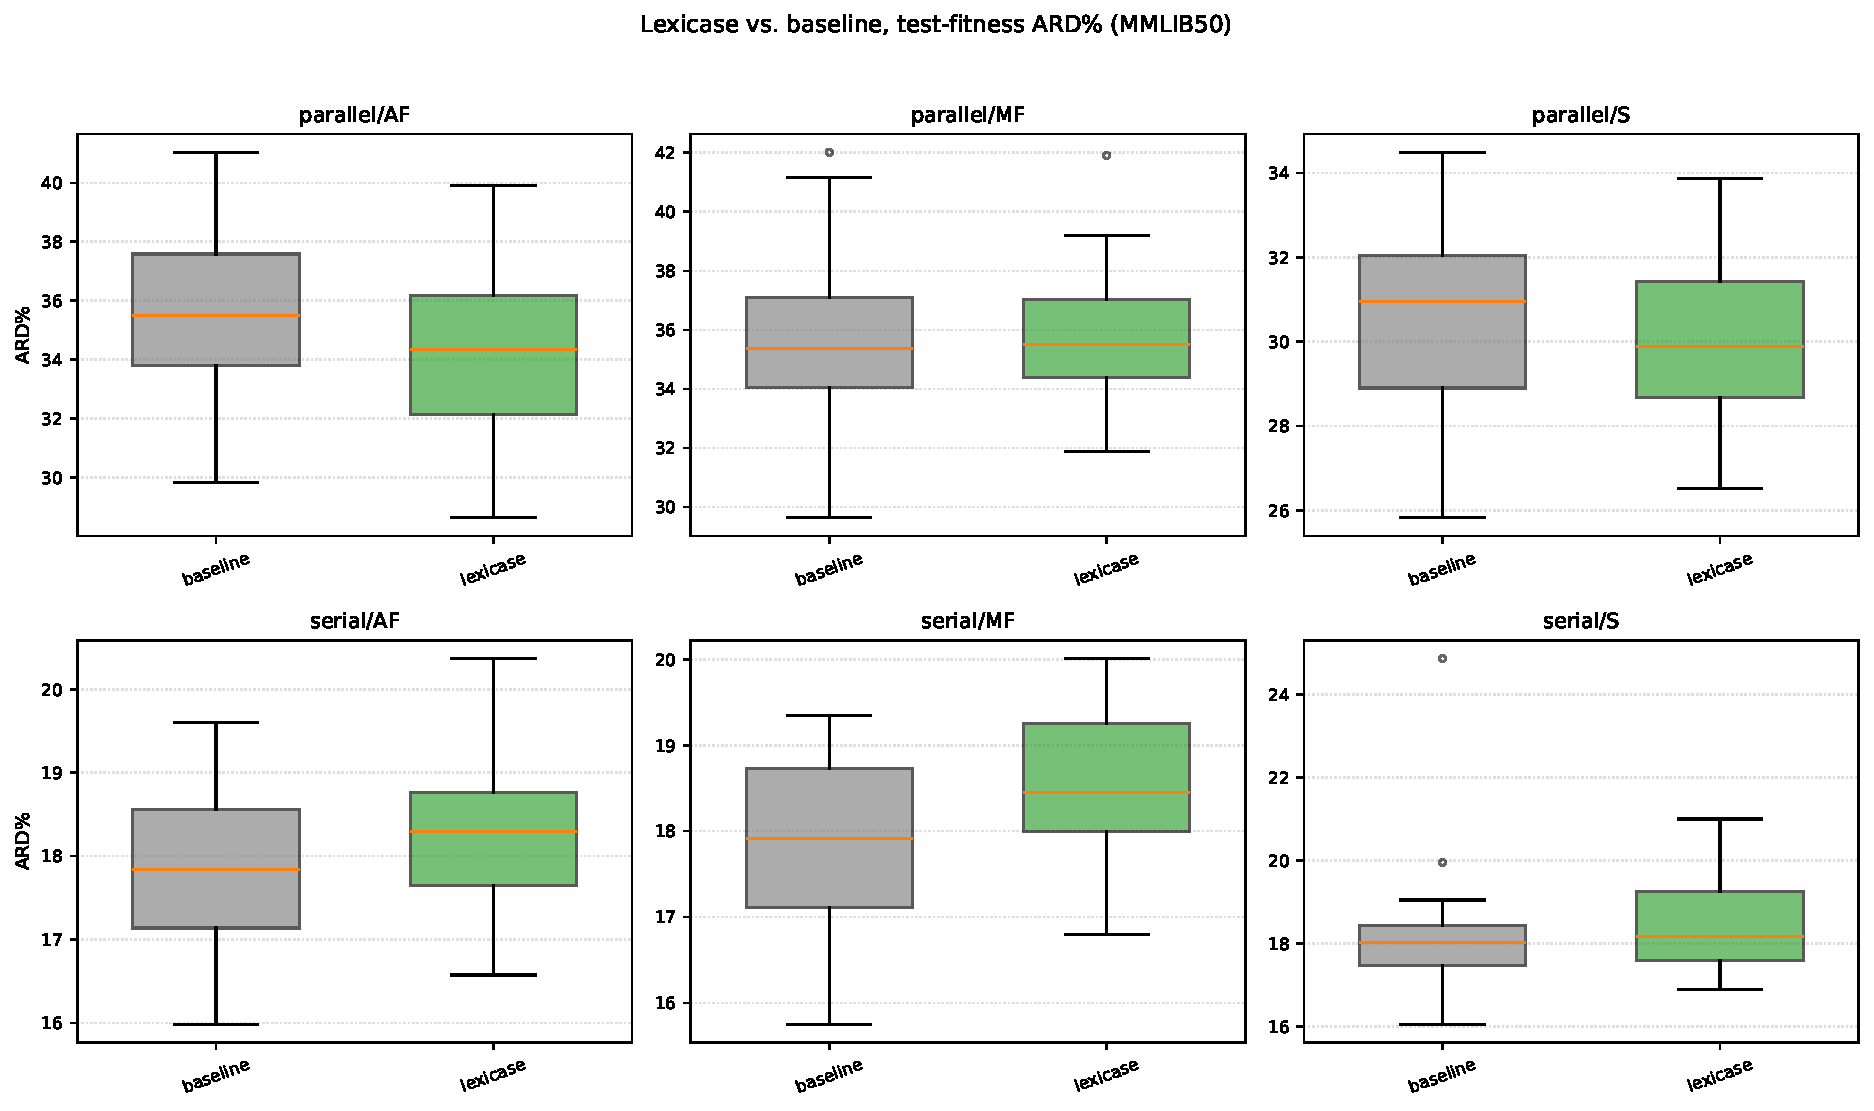
\includegraphics[width=0.95\textwidth]{img/generated/lexicase_boxplot_mmlib50.pdf}
  \caption{Distribution of test-fitness ARD\%, lexicase vs.\ baseline,
  MMLIB50, one panel per (SGS, strategy) cell, 30 seeds per box. Generated
  directly from the raw per-seed result files by
  \texttt{yuantian/experiments/generate\_thesis\_plots.py}.}
  \label{fig:lexicase-boxplot}
\end{figure}

\begin{figure}[htbp]
  \centering
  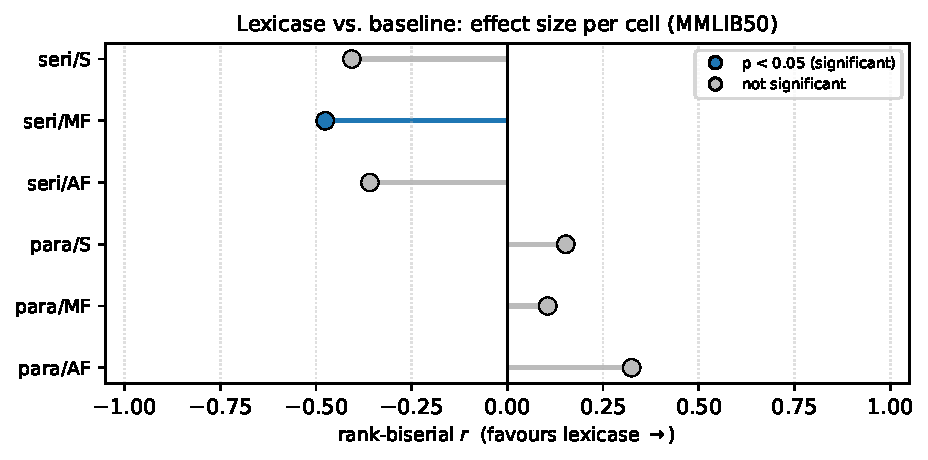
\includegraphics[width=0.85\textwidth]{img/generated/lexicase_effectsize_mmlib50.pdf}
  \caption[Effect-size summary, lexicase vs.\ baseline]{Effect-size summary,
  lexicase vs.\ baseline, MMLIB50: matched rank-biserial correlation $r$ per
  (SGS, strategy) cell (positive favours lexicase), filled markers denote
  $p<0.05$. A full critical-difference diagram is not drawn for this
  two-condition comparison, since with only two conditions the Nemenyi
  post-hoc a CD diagram relies on degenerates to the paired Wilcoxon test
  already reported in Table~\ref{tab:lexicase-significance}; this per-cell
  effect-size view is the more informative visual summary for $k=2$.}
  \label{fig:lexicase-cd}
\end{figure}

\begin{table}[htbp]
  \centering
  \small
  \shrinktofit{%
  \caption[Lexicase vs.\ baseline on MMLIB100]{Mean ARD\% (\%), baseline
  vs.\ epsilon-lexicase selection, MMLIB100 (scalability validation),
  $n=30$ seeds per cell.}
  \label{tab:lexicase-vs-baseline-mmlib100}
  \begin{tabular}{llrrrr}
    \toprule
    \textbf{SGS} & \textbf{Strategy} & \textbf{Baseline (test)} & \textbf{Lexicase (test)} & \textbf{Baseline (train)} & \textbf{Lexicase (train)} \\
    \midrule
    Parallel & AF & 25.40 & 26.24\,\ArrWorse & 19.21 & 20.18\,\ArrWorse \\
    Parallel & MF & 28.04 & 28.00\,\ArrBetter & 20.75 & 20.82\,\ArrWorse \\
    Parallel & S  & 23.28 & 22.76\,\ArrBetter & 16.55 & 16.43\,\ArrBetter \\
    Serial   & AF & 14.64 & 15.37\,\ArrWorse & 12.38 & 12.00\,\ArrBetter \\
    Serial   & MF & 14.88 & 15.39\,\ArrWorse & 12.42 & 11.95\,\ArrBetter \\
    Serial   & S  & 14.68 & 14.38\,\ArrBetter & 12.58 & 12.30\,\ArrBetter \\
    \bottomrule
  \end{tabular}%
  }
\end{table}

\begin{table}[htbp]
  \centering
  \small
  \shrinktofit{%
  \caption[Statistical significance: lexicase vs.\ baseline, MMLIB100]{Two-sided
  paired Wilcoxon signed-rank test and matched rank-biserial effect size
  $r$, lexicase vs.\ baseline, MMLIB100.}
  \label{tab:lexicase-significance-mmlib100}
  \begin{tabular}{lllrrl}
    \toprule
    \textbf{SGS} & \textbf{Strategy} & \textbf{Split} & \textbf{$p$} & \textbf{$r$} & \textbf{Verdict} \\
    \midrule
    Parallel & AF & Train & 0.0000 & $-0.966$ & Significant, favours baseline \\
    Parallel & AF & Test  & 0.0523 & $-0.406$ & Not significant (borderline, favours baseline) \\
    Parallel & MF & Train & 0.3818 & $-0.187$ & Not significant \\
    Parallel & MF & Test  & 0.5291 & $+0.135$ & Not significant \\
    Parallel & S  & Train & 0.2621 & $+0.239$ & Not significant \\
    Parallel & S  & Test  & 0.1909 & $+0.277$ & Not significant \\
    Serial   & AF & Train & 0.0001 & $+0.776$ & Significant, favours lexicase \\
    Serial   & AF & Test  & 0.0054 & $-0.570$ & Significant, favours baseline \\
    Serial   & MF & Train & 0.0000 & $+0.854$ & Significant, favours lexicase \\
    Serial   & MF & Test  & 0.0427 & $-0.424$ & Significant, favours baseline \\
    Serial   & S  & Train & 0.0010 & $+0.665$ & Significant, favours lexicase \\
    Serial   & S  & Test  & 0.1909 & $+0.277$ & Not significant \\
    \bottomrule
  \end{tabular}%
  }
\end{table}

\begin{figure}[htbp]
  \centering
  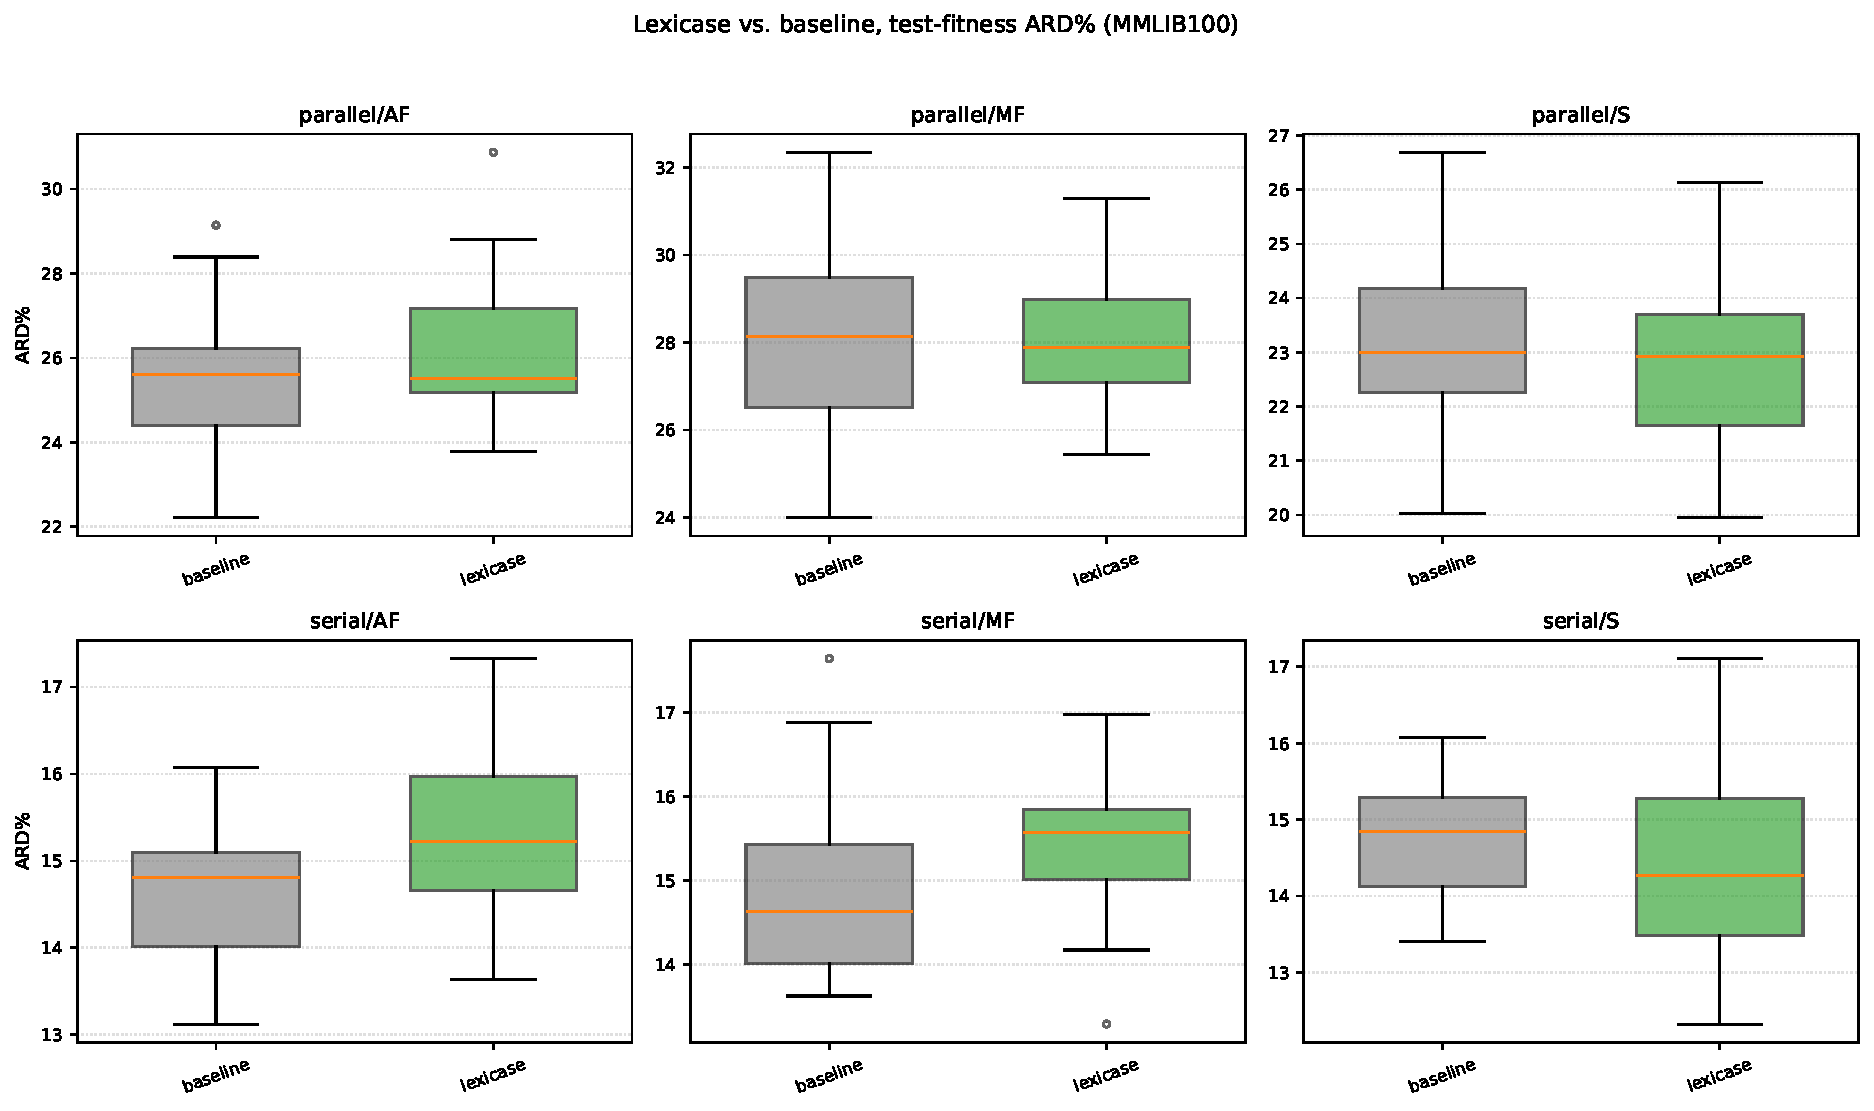
\includegraphics[width=0.95\textwidth]{img/generated/lexicase_boxplot_mmlib100.pdf}
  \caption{Distribution of test-fitness ARD\%, lexicase vs.\ baseline,
  MMLIB100, same layout as Figure~\ref{fig:lexicase-boxplot}.}
  \label{fig:lexicase-boxplot-mmlib100}
\end{figure}

\begin{figure}[htbp]
  \centering
  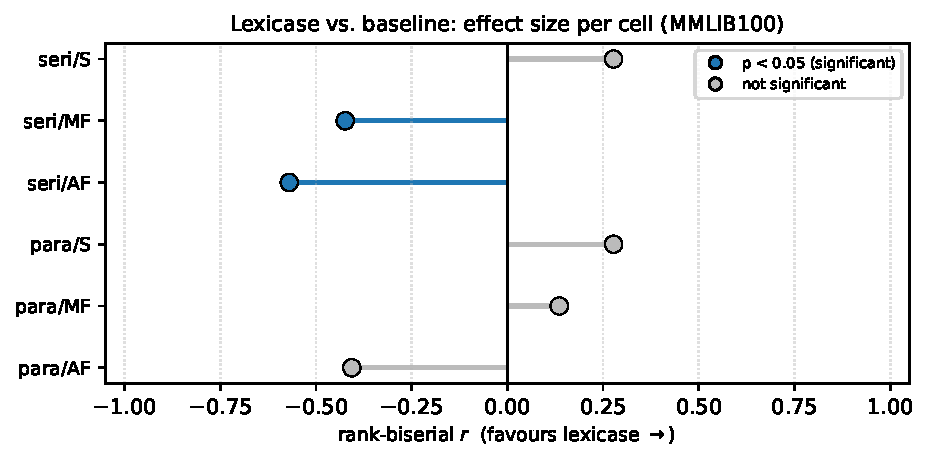
\includegraphics[width=0.85\textwidth]{img/generated/lexicase_effectsize_mmlib100.pdf}
  \caption[Effect-size summary, lexicase vs.\ baseline, MMLIB100]{Effect-size
  summary, lexicase vs.\ baseline, MMLIB100: compare against
  Figure~\ref{fig:lexicase-cd}'s MMLIB50 panel to see the serial-SGS cells
  shift further into unfavourable territory at the larger scale.}
  \label{fig:lexicase-cd-mmlib100}
\end{figure}

\changed{The fully powered comparison confirms, and considerably sharpens,
the pilot's qualitative finding.} On
\emph{training} fitness, lexicase selection shows a clear and consistent,
but direction-dependent, effect: under serial SGS it significantly
outperforms the baseline in all three decision strategies (activity-first
$p=0.0030$, $r=0.604$; mode-first $p=0.0248$, $r=0.467$; simultaneous
$p<0.0001$, $r=0.888$), while under parallel SGS it significantly
\emph{underperforms} the baseline in two of three strategies
(activity-first $p=0.0113$, mode-first $p=0.0327$, both favouring the
baseline). On \emph{test} fitness, \changed{the results} change again: the serial
advantage that was so clear on training data does not reliably survive the
generalisation step, one serial cell (mode-first) reverses into a
significant loss ($p=0.0252$, $r=-0.476$), a second (simultaneous) is a
borderline, non-significant loss ($p=0.0519$), and only the parallel cells
retain a (non-significant) direction favourable to lexicase. Averaged
across all six cells, lexicase's average rank on test fitness (2.33) ties
exactly with the baseline's own (2.33), well behind local search's 1.50
(Section~\ref{subsec:final-comparison}).

\changed{This is a more nuanced result than either the pilot screen or the
original motivation for trying lexicase selection anticipated.} Lexicase
selection reliably finds
GP trees that fit the specific training instances better, an effect large
and consistent enough, under serial SGS especially, to leave little doubt
that the mechanism is doing something real to the search. That advantage,
however, does not transfer reliably to the held-out test instances, and
under serial SGS it can reverse outright. \changed{In practical terms, the
two selection mechanisms are good at different goals: lexicase selection
is the better choice when the aim is to solve a fixed, known set of
instances as well as possible, which is exactly what training fitness
measures, whereas the goal pursued by a hyper-heuristic is a rule that
generalises to unseen instances, so the improvement must appear on the
test data, and there the tournament baseline remains at least as good.} A plausible reading is mild
overfitting: lexicase's case-by-case elimination rewards individuals that
handle the specific quirks of the 30 training instances well, including
quirks that do not generalise, whereas tournament selection's
aggregate-fitness pressure is, if anything, a coarser, more
generalisation-friendly signal precisely because it cannot fixate on any
single instance. Why this reversal is concentrated in serial SGS and not
parallel SGS is a genuinely open question; a candidate explanation, matched
to what changes about decoding between the two, is discussed in
Section~\ref{subsec:localsearch-eval} and returned to in
Chapter~\ref{chap:conclusion}. \changed{Overall, MMLIB50 does not offer
clean evidence that lexicase selection alone is an unambiguous improvement
over the baseline.}

\textbf{Scalability validation.} Table~\ref{tab:lexicase-significance-mmlib100}
answers the question posed above directly: the training-fitness advantage
under serial SGS not only persists at MMLIB100's larger instance size, it
remains significant in all three decision strategies with comparable
effect sizes to MMLIB50 ($r=0.665$--$0.854$, against $r=0.467$--$0.888$ on
MMLIB50). \changed{The test-fitness results, however, do not merely hold
steady, they \emph{sharpen in the unfavourable direction}:} on MMLIB50 only one of
three serial cells reached significance on test fitness (mode-first,
$p=0.0252$); on MMLIB100, two of three do (activity-first, $p=0.0054$,
$r=-0.570$; mode-first, $p=0.0427$, $r=-0.424$), and the third
(simultaneous) sits at a non-significant but still unfavourable-leaning
$r=+0.277$ (a sign flip from MMLIB50's $r=-0.406$, so this one cell alone
does not confirm the pattern). Read together, MMLIB100 strengthens rather
than weakens the mild-overfitting interpretation offered \changed{above}: a larger
instance size did not give lexicase's serial-SGS training advantage more
room to generalise, if anything the training/test gap widened. This is the
clearer of this chapter's two scalability findings: MMLIB100 does not just
fail to overturn the MMLIB50 concern about lexicase's generalisation under
serial SGS, it actively corroborates it.

\changedB{For a concrete picture of the priority rules these statistics
summarise, Figure~\ref{fig:lexicase-evolved-tree} shows a compact rule pair
evolved under lexicase selection. Because lexicase changes only the selection
operator and not the terminal set, the evolved trees draw purely on the
standard baseline vocabulary, so, unlike the NR-aware rule of
Figure~\ref{fig:nr-evolved-tree}, no terminal is highlighted: the difference
lexicase makes is in which individuals survive, not in what they can
express.} \changedC{The pair is also readable once its functionally neutral
code is stripped away: in the activity tree, \texttt{LF}\,\%\,\texttt{LF}
(protected division of a terminal by itself) is the constant $1$ and
$\max(\texttt{LF}, \texttt{LF})$ is simply \texttt{LF}, both typical of the
neutral material GP trees accumulate. What remains is driven almost
entirely by the CPM time-window terminals \texttt{LS} and \texttt{LF}:
since the SGS schedules the activity with the \emph{smallest} rule value
(Section~\ref{subsec:sgs}), the rule prefers activities whose
precedence-feasible window closes early, with the $\texttt{TSC}/\texttt{LF}$
term additionally favouring activities with many transitive successors. The
mode tree is a product of \texttt{GRD}, mode duration and average
requirement, so it prefers short modes with light resource demands.}

\begin{figure}[htbp]
  \centering
  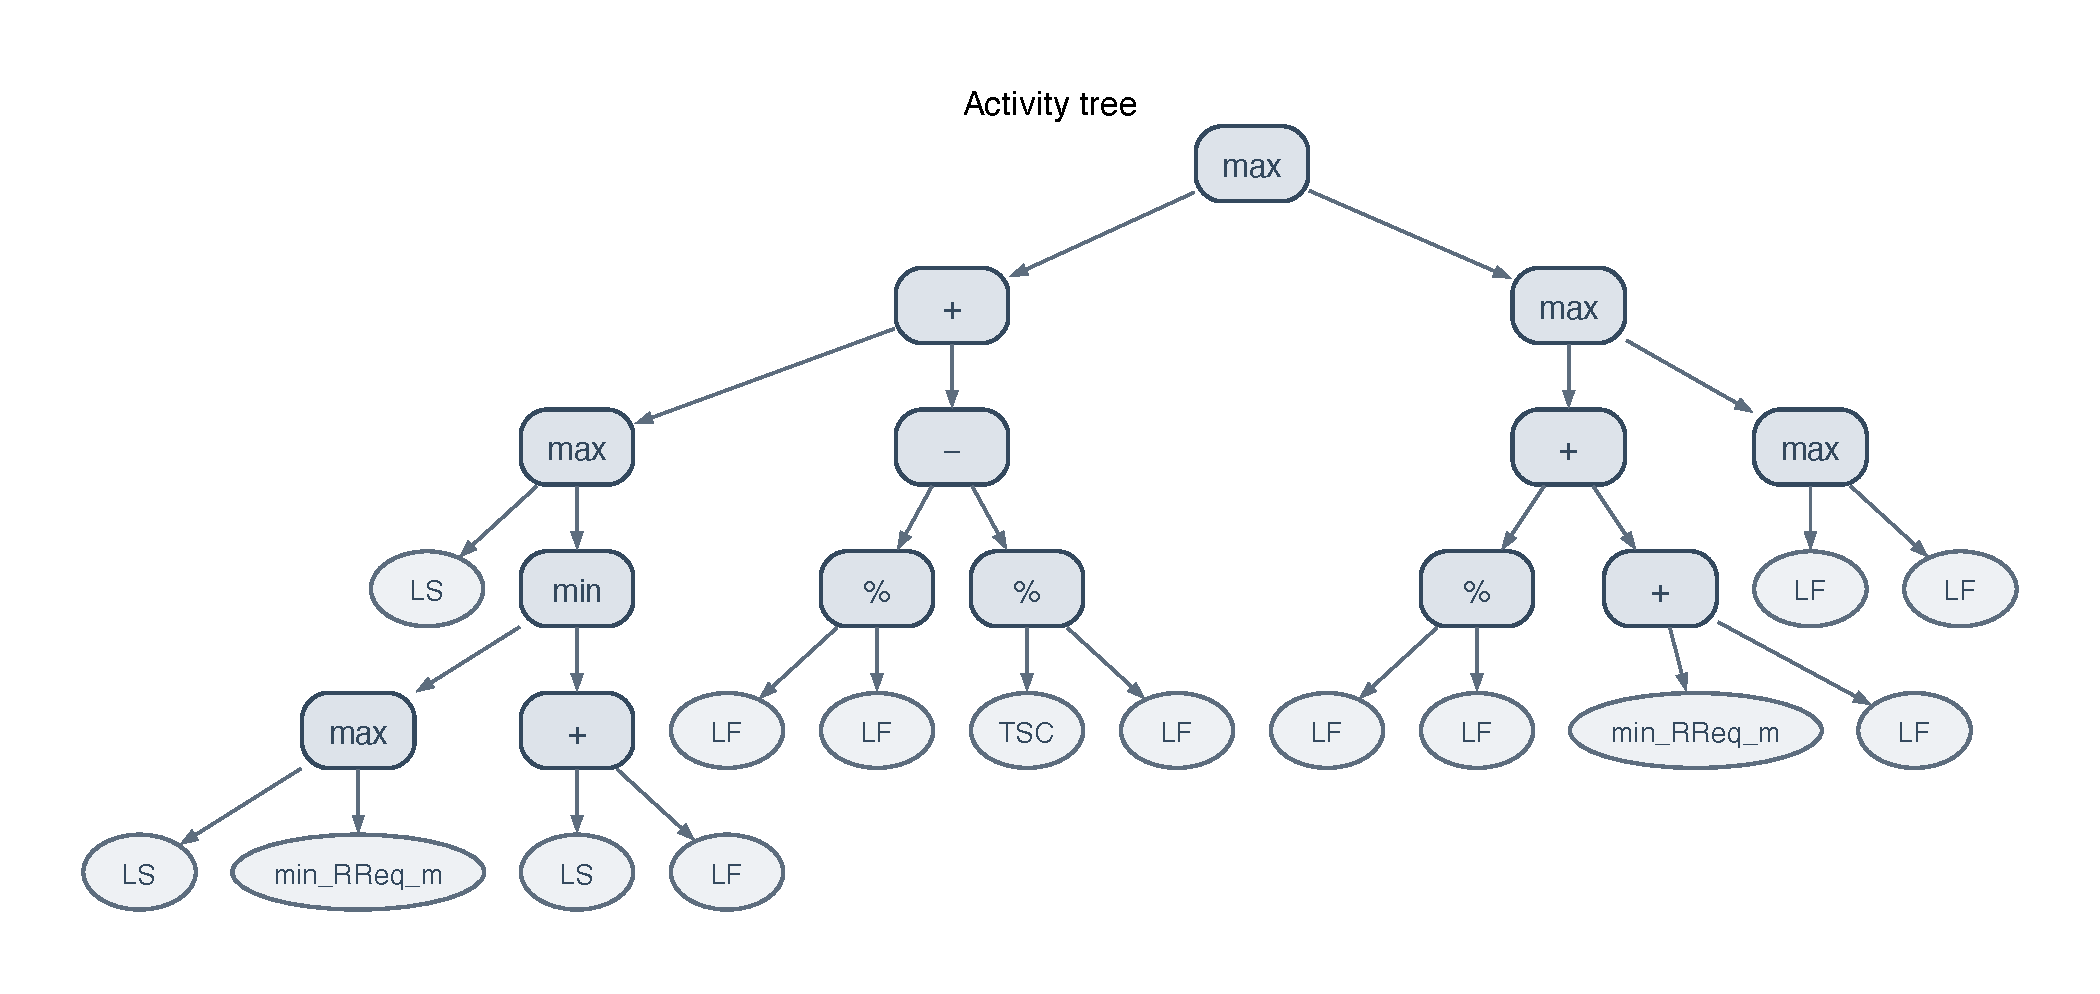
\includegraphics[width=0.98\textwidth]{img/generated/gp_tree_lexicase_activity.pdf}\\[1.5ex]
  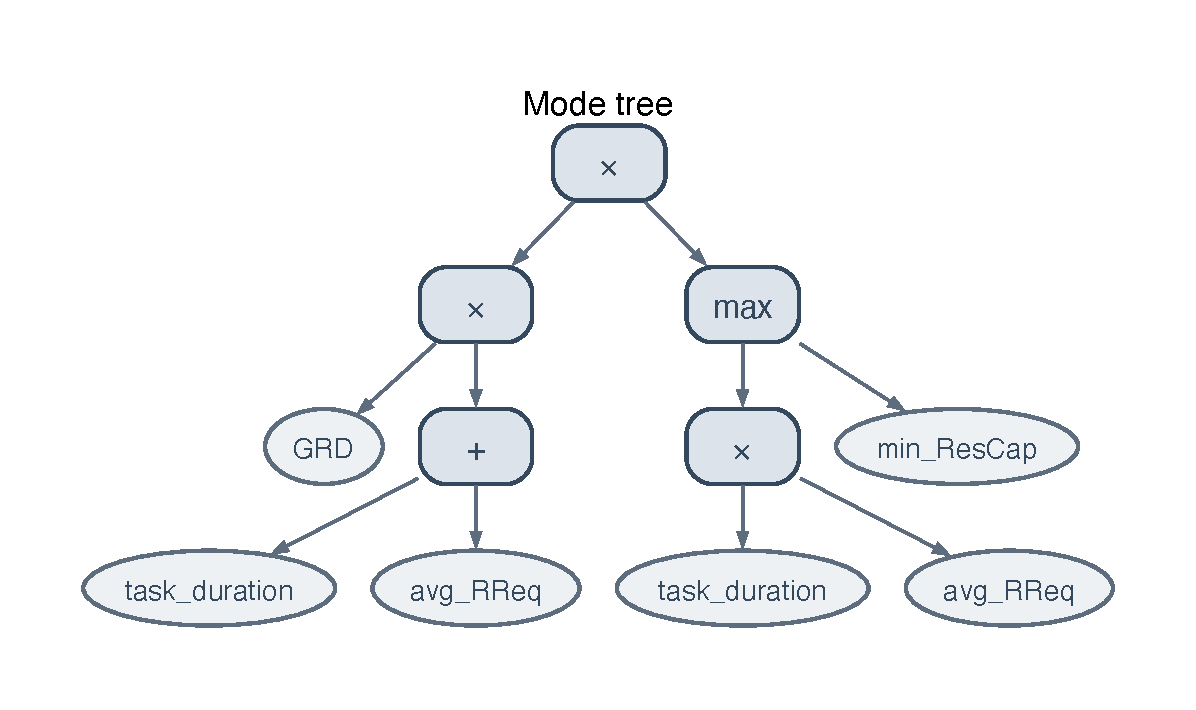
\includegraphics[width=0.5\textwidth]{img/generated/gp_tree_lexicase_mode.pdf}
  \caption[Evolved rule pair under lexicase selection]{\changedB{A compact
  evolved rule pair under lexicase selection (parallel/activity-first,
  MMLIB100), selected as the smallest feasible individual. Top: the activity
  tree; bottom: the mode tree. Operator nodes are blue and terminals grey;
  the standard baseline terminal set is used throughout (no NR terminals).
  Operators as in Figure~\ref{fig:nr-evolved-tree}.}}
  \label{fig:lexicase-evolved-tree}
\end{figure}

\subsection{Comprehensive evaluation of local search with critical path}
\label{subsec:localsearch-eval}

Local search is an attractive complement to a GP-evolved priority rule
because the two operate at different levels: the GP tree decides, in
general, which activity and mode to prefer, while the \changed{Baldwinian}, per-elite
refinement step defined in full in Section~\ref{subsec:localsearch-definition}
can exploit information specific to the one schedule that tree actually
produced on this instance. This section evaluates that mechanism, unchanged,
against the baseline at full statistical power.

\begin{table}[htbp]
  \centering
  \small
  \shrinktofit{%
  \caption[Local search vs.\ baseline on MMLIB50]{Mean ARD\% (\%), baseline
  vs.\ critical-path local search, MMLIB50, $n=30$ seeds per cell.}
  \label{tab:localsearch-vs-baseline-mmlib50}
  \begin{tabular}{llrrrr}
    \toprule
    \textbf{SGS} & \textbf{Strategy} & \textbf{Baseline (test)} & \textbf{Local search (test)} & \textbf{Baseline (train)} & \textbf{Local search (train)} \\
    \midrule
    Parallel & AF & 35.77 & 33.64\,\ArrBetter & 15.94 & 15.72\,\ArrBetter \\
    Parallel & MF & 35.78 & 35.57\,\ArrBetter & 16.61 & 16.87\,\ArrWorse \\
    Parallel & S  & 30.43 & 29.79\,\ArrBetter & 14.20 & 13.95\,\ArrBetter \\
    Serial   & AF & 17.81 & 18.24\,\ArrWorse &  9.83 &  9.85\,\ArrWorse \\
    Serial   & MF & 17.89 & 18.37\,\ArrWorse &  9.82 &  9.87\,\ArrWorse \\
    Serial   & S  & 18.08 & 17.77\,\ArrBetter & 10.29 & 10.29\,\ArrSame \\
    \bottomrule
  \end{tabular}%
  }
\end{table}

\begin{table}[htbp]
  \centering
  \small
  \shrinktofit{%
  \caption[Descriptive statistics: local search vs.\ baseline]{Standard
  deviation accompanying Table~\ref{tab:localsearch-vs-baseline-mmlib50}.
  Feasibility rate is 1.00 for both conditions in every cell.}
  \label{tab:localsearch-descriptive-stats}
  \begin{tabular}{lllrr}
    \toprule
    \textbf{SGS} & \textbf{Strategy} & \textbf{Split} & \textbf{Baseline std} & \textbf{Local search std} \\
    \midrule
    Parallel & AF & Train & 0.58 & 0.55 \\
    Parallel & AF & Test  & 2.74 & 2.61 \\
    Parallel & MF & Train & 0.66 & 0.70 \\
    Parallel & MF & Test  & 2.77 & 2.41 \\
    Parallel & S  & Train & 0.64 & 0.57 \\
    Parallel & S  & Test  & 2.24 & 2.34 \\
    Serial   & AF & Train & 0.25 & 0.25 \\
    Serial   & AF & Test  & 0.91 & 0.91 \\
    Serial   & MF & Train & 0.26 & 0.25 \\
    Serial   & MF & Test  & 0.91 & 0.94 \\
    Serial   & S  & Train & 0.24 & 0.23 \\
    Serial   & S  & Test  & 1.51 & 0.74 \\
    \bottomrule
  \end{tabular}%
  }
\end{table}

\begin{table}[htbp]
  \centering
  \small
  \shrinktofit{%
  \caption[Statistical significance: local search vs.\ baseline]{Two-sided
  paired Wilcoxon signed-rank test and matched rank-biserial effect size
  $r$ (positive favours local search), local search vs.\ baseline, MMLIB50,
  $n=30$ per cell.}
  \label{tab:localsearch-significance}
  \begin{tabular}{lllrrl}
    \toprule
    \textbf{SGS} & \textbf{Strategy} & \textbf{Split} & \textbf{$p$} & \textbf{$r$} & \textbf{Verdict} \\
    \midrule
    Parallel & AF & Train & 0.0803 & $+0.368$ & Not significant \\
    Parallel & AF & Test  & 0.0026 & $+0.613$ & Significant, favours local search \\
    Parallel & MF & Train & 0.1191 & $-0.329$ & Not significant \\
    Parallel & MF & Test  & 0.9677 & $+0.011$ & Not significant \\
    Parallel & S  & Train & 0.1241 & $+0.325$ & Not significant \\
    Parallel & S  & Test  & 0.1981 & $+0.273$ & Not significant \\
    Serial   & AF & Train & 0.8553 & $-0.041$ & Not significant \\
    Serial   & AF & Test  & 0.1274 & $-0.324$ & Not significant \\
    Serial   & MF & Train & 0.4645 & $-0.157$ & Not significant \\
    Serial   & MF & Test  & 0.0961 & $-0.351$ & Not significant \\
    Serial   & S  & Train & 0.8078 & $+0.054$ & Not significant \\
    Serial   & S  & Test  & 0.6263 & $+0.105$ & Not significant \\
    \bottomrule
  \end{tabular}%
  }
\end{table}

\begin{figure}[htbp]
  \centering
  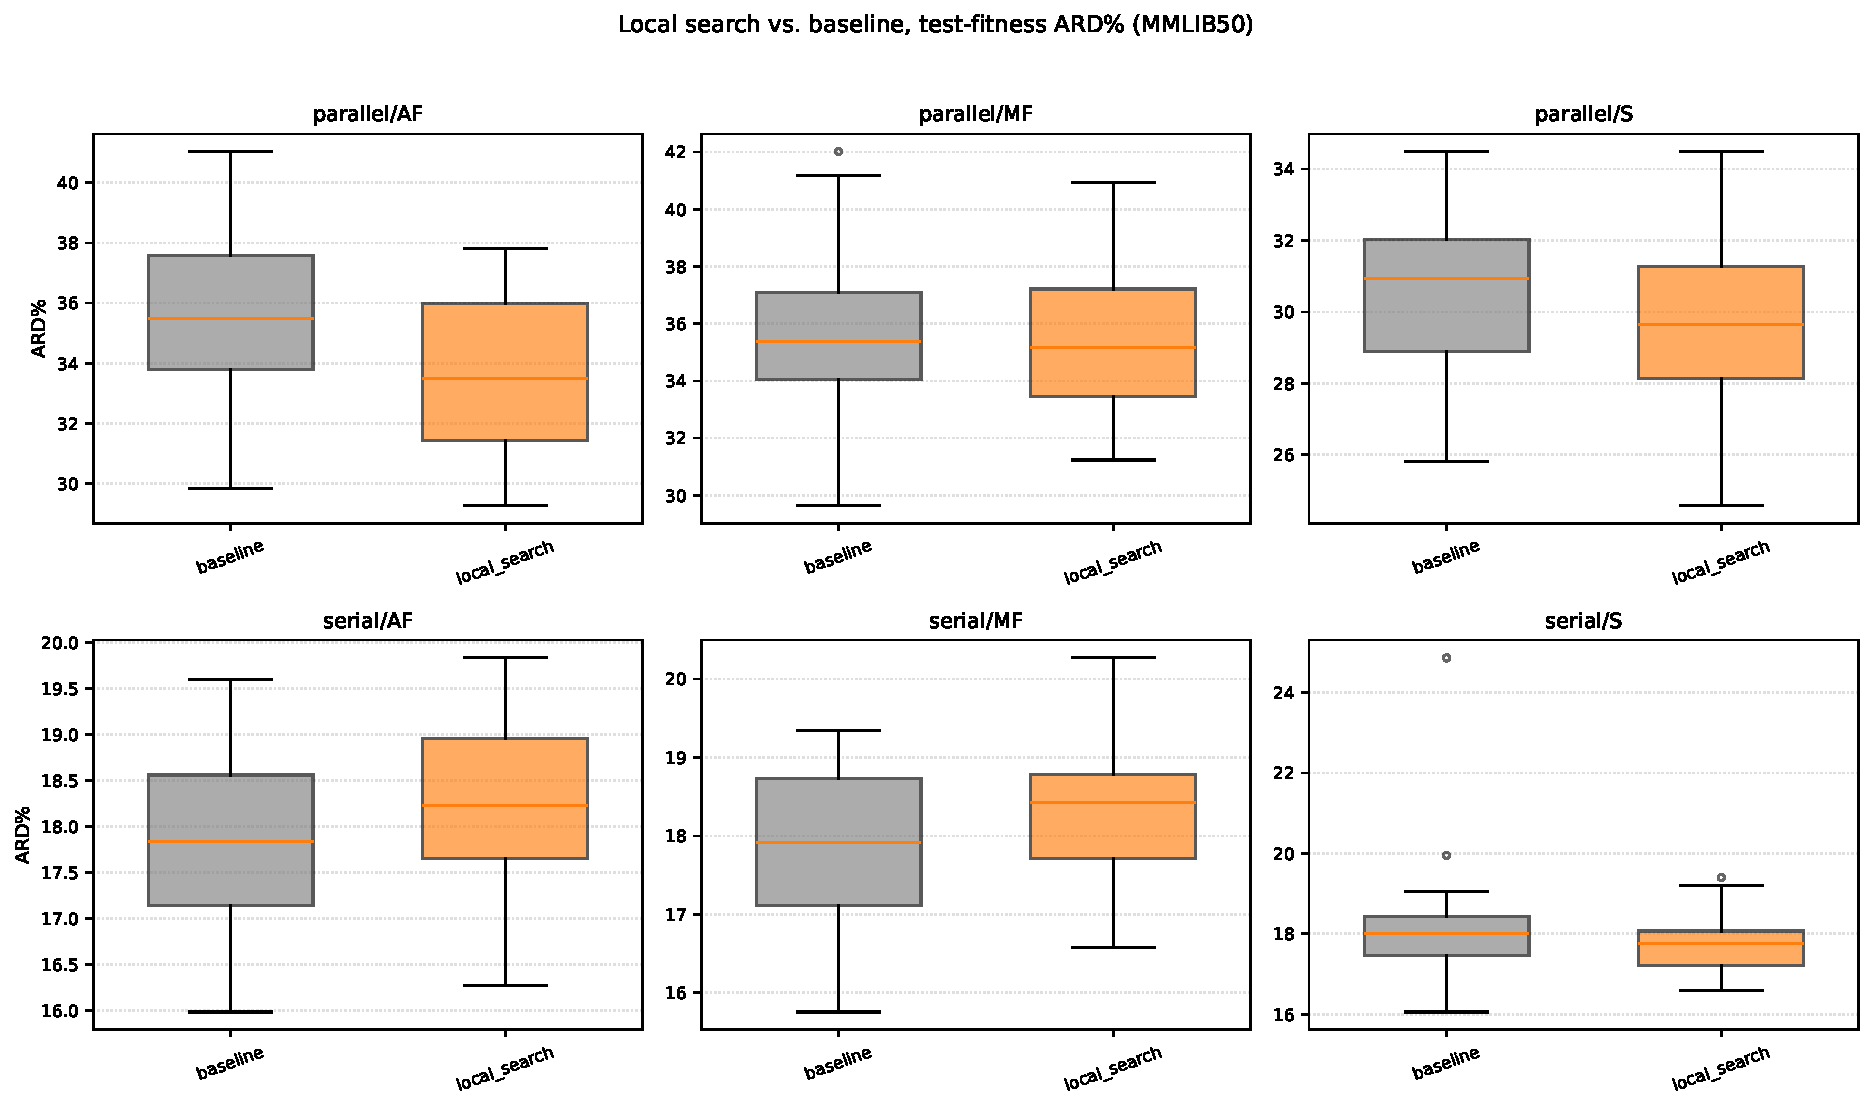
\includegraphics[width=0.95\textwidth]{img/generated/localsearch_boxplot_mmlib50.pdf}
  \caption{Distribution of test-fitness ARD\%, local search vs.\ baseline,
  MMLIB50, one panel per (SGS, strategy) cell, 30 seeds per box.}
  \label{fig:localsearch-boxplot}
\end{figure}

\begin{figure}[htbp]
  \centering
  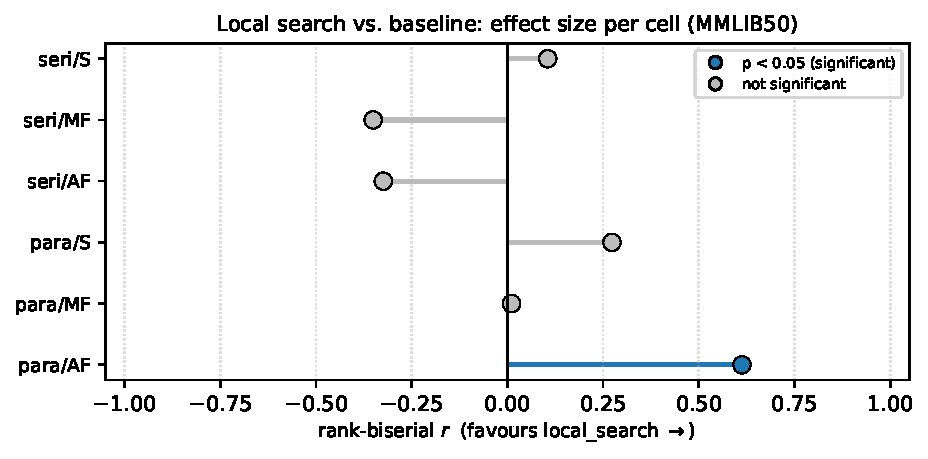
\includegraphics[width=0.85\textwidth]{img/generated/localsearch_effectsize_mmlib50.pdf}
  \caption[Effect-size summary, local search vs.\ baseline]{Effect-size
  summary, local search vs.\ baseline, MMLIB50: matched rank-biserial
  correlation $r$ per (SGS, strategy) cell (positive favours local search),
  filled markers denote $p<0.05$; see Figure~\ref{fig:lexicase-cd}'s caption
  for why a per-cell effect-size plot, not a Nemenyi CD diagram, is used for
  this two-condition comparison.}
  \label{fig:localsearch-cd}
\end{figure}

\begin{table}[htbp]
  \centering
  \small
  \shrinktofit{%
  \caption[Local search vs.\ baseline on MMLIB100]{Mean ARD\% (\%), baseline
  vs.\ critical-path local search, MMLIB100 (scalability validation), $n=30$
  seeds per cell.}
  \label{tab:localsearch-vs-baseline-mmlib100}
  \begin{tabular}{llrrrr}
    \toprule
    \textbf{SGS} & \textbf{Strategy} & \textbf{Baseline (test)} & \textbf{Local search (test)} & \textbf{Baseline (train)} & \textbf{Local search (train)} \\
    \midrule
    Parallel & AF & 25.40 & 25.90\,\ArrWorse & 19.21 & 19.45\,\ArrWorse \\
    Parallel & MF & 28.04 & 28.40\,\ArrWorse & 20.75 & 21.01\,\ArrWorse \\
    Parallel & S  & 23.28 & 23.60\,\ArrWorse & 16.55 & 16.79\,\ArrWorse \\
    Serial   & AF & 14.64 & 14.71\,\ArrWorse & 12.38 & 12.38\,\ArrSame \\
    Serial   & MF & 14.88 & 14.78\,\ArrBetter & 12.42 & 12.35\,\ArrBetter \\
    Serial   & S  & 14.68 & 14.68\,\ArrSame & 12.58 & 12.75\,\ArrWorse \\
    \bottomrule
  \end{tabular}%
  }
\end{table}

\begin{table}[htbp]
  \centering
  \small
  \shrinktofit{%
  \caption[Statistical significance: local search vs.\ baseline, MMLIB100]{Two-sided
  paired Wilcoxon signed-rank test and matched rank-biserial effect size
  $r$, local search vs.\ baseline, MMLIB100.}
  \label{tab:localsearch-significance-mmlib100}
  \begin{tabular}{lllrrl}
    \toprule
    \textbf{SGS} & \textbf{Strategy} & \textbf{Split} & \textbf{$p$} & \textbf{$r$} & \textbf{Verdict} \\
    \midrule
    Parallel & AF & Train & 0.3285 & $-0.209$ & Not significant \\
    Parallel & AF & Test  & 0.2621 & $-0.239$ & Not significant \\
    Parallel & MF & Train & 0.0699 & $-0.381$ & Not significant \\
    Parallel & MF & Test  & 0.2367 & $-0.252$ & Not significant \\
    Parallel & S  & Train & 0.2286 & $-0.256$ & Not significant \\
    Parallel & S  & Test  & 0.5561 & $-0.127$ & Not significant \\
    Serial   & AF & Train & 0.7000 & $-0.084$ & Not significant \\
    Serial   & AF & Test  & 0.8872 & $-0.032$ & Not significant \\
    Serial   & MF & Train & 0.5158 & $+0.140$ & Not significant \\
    Serial   & MF & Test  & 0.9193 & $+0.024$ & Not significant \\
    Serial   & S  & Train & 0.0803 & $-0.368$ & Not significant \\
    Serial   & S  & Test  & 0.8022 & $+0.054$ & Not significant \\
    \bottomrule
  \end{tabular}%
  }
\end{table}

\begin{figure}[htbp]
  \centering
  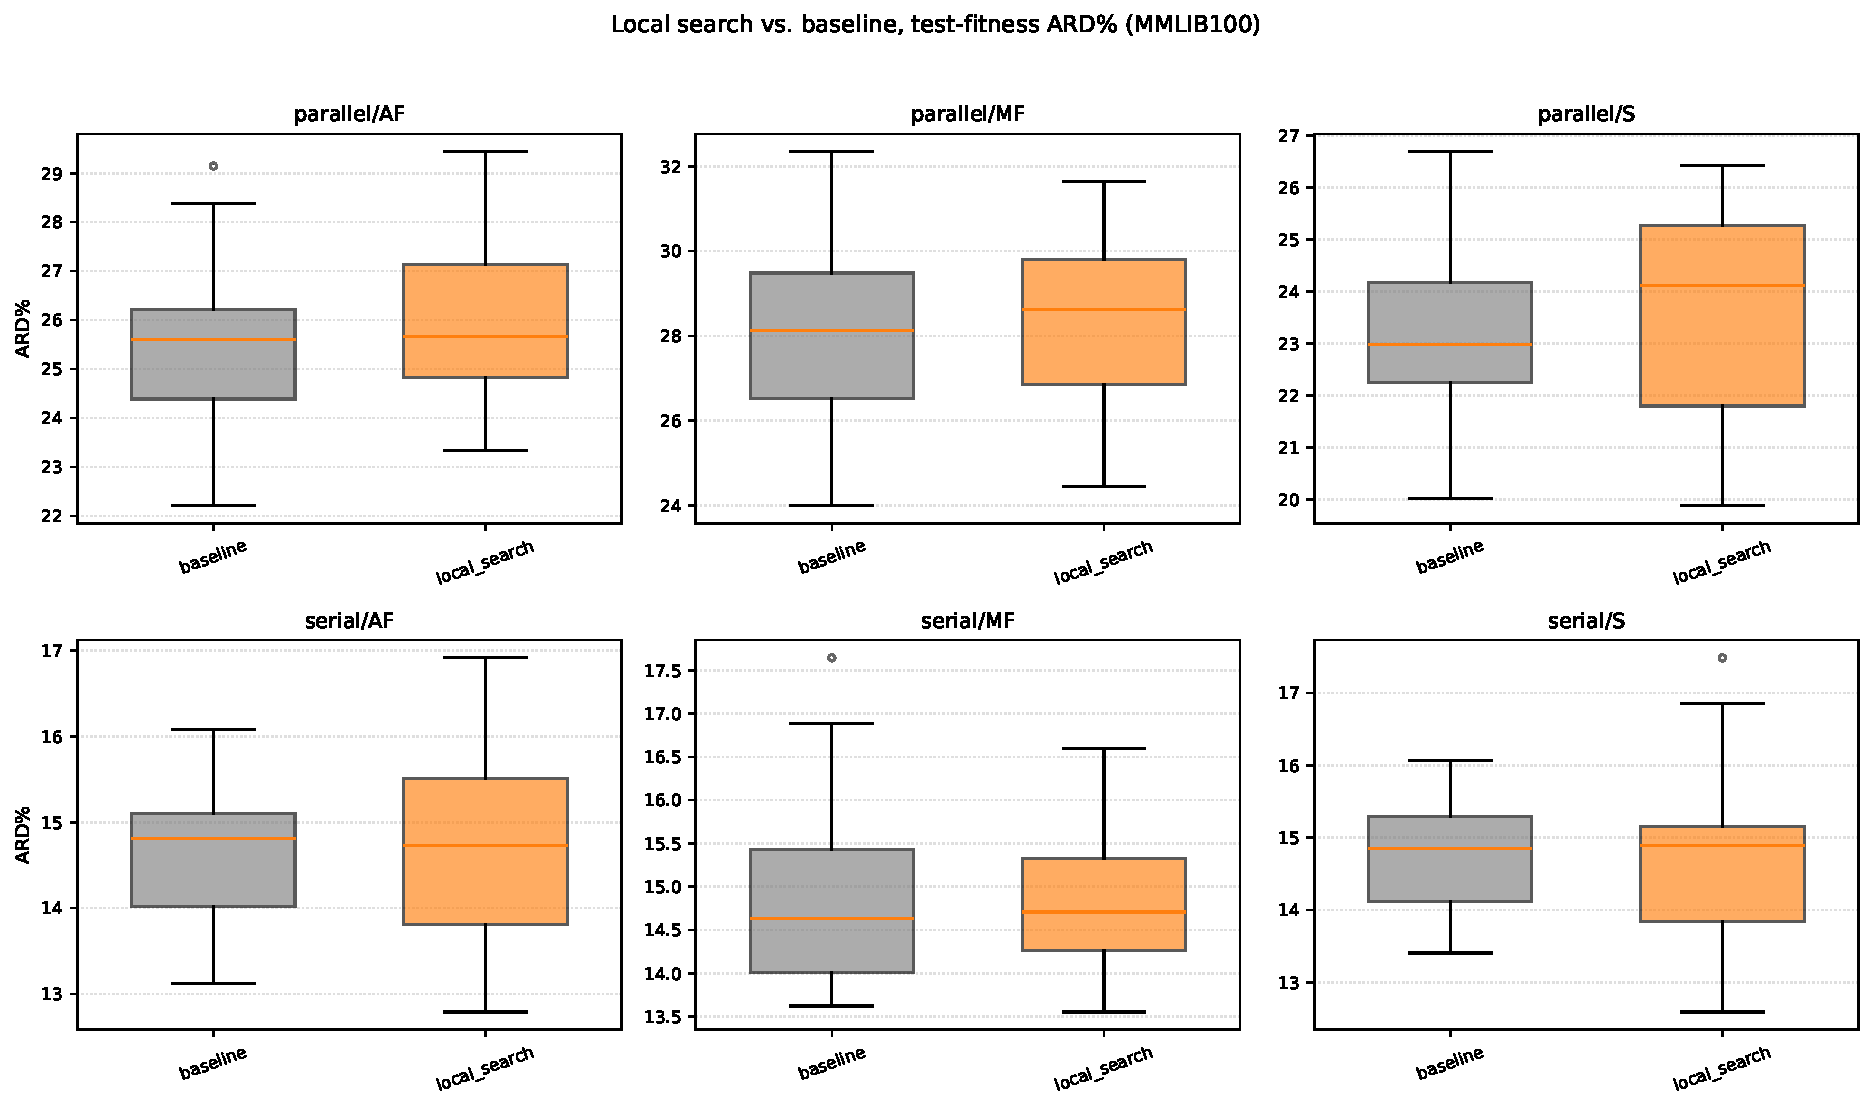
\includegraphics[width=0.95\textwidth]{img/generated/localsearch_boxplot_mmlib100.pdf}
  \caption{Distribution of test-fitness ARD\%, local search vs.\ baseline,
  MMLIB100, same layout as Figure~\ref{fig:localsearch-boxplot}.}
  \label{fig:localsearch-boxplot-mmlib100}
\end{figure}

\begin{figure}[htbp]
  \centering
  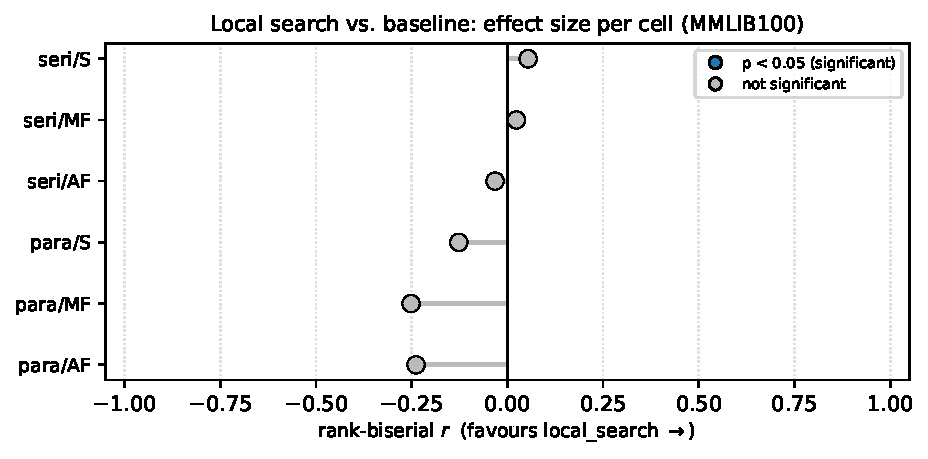
\includegraphics[width=0.85\textwidth]{img/generated/localsearch_effectsize_mmlib100.pdf}
  \caption[Effect-size summary, local search vs.\ baseline, MMLIB100]{Effect-size
  summary, local search vs.\ baseline, MMLIB100: every cell sits much closer
  to zero than its MMLIB50 counterpart in Figure~\ref{fig:localsearch-cd},
  visualising the loss of the one significant MMLIB50 win.}
  \label{fig:localsearch-cd-mmlib100}
\end{figure}

Table~\ref{tab:localsearch-significance} tells a more qualified story than
the section's motivation might suggest. Exactly one of the twelve
train/test comparisons reaches significance: parallel/activity-first test
fitness improves from 35.77\% to 33.64\% ($p=0.0026$, $r=0.613$, a
moderately large effect). No other cell, train or test, serial or parallel,
reaches conventional significance, and the \emph{direction} of the
(non-significant) effect itself depends systematically on SGS: all three
parallel test cells favour local search (activity-first significantly so,
mode-first and simultaneous non-significantly), while two of the three
serial test cells favour the baseline instead. Averaged across all six
cells, local search nonetheless achieves the best average test-fitness rank
of any of the four directly comparable conditions (1.50, ahead of baseline
and lexicase at 2.33 each and hybrid at 3.83,
Section~\ref{subsec:final-comparison}), driven by consistently
favourable, even if individually non-significant, performance under
parallel SGS.

A plausible explanation for this SGS-dependent pattern lies in how much
room each decoding scheme leaves for a post-hoc, per-instance refinement
step to exploit. Parallel SGS advances a single global clock and commits
several activities to the same time step at once, which tends to leave more
slack, and more genuinely improvable local structure, in the resulting
schedule for the resource-shift move to find and exploit. Serial SGS's
greedy, one-activity-at-a-time construction already resolves many of the
same local trade-offs as it builds the schedule, leaving comparatively
little for a subsequent hill-climb to improve on, and occasionally
disturbing a schedule that was already close to locally optimal for that
decoding scheme. This reading is consistent with, and offers one candidate
explanation for, Section~\ref{subsec:lexicase-eval}'s otherwise puzzling
observation that lexicase's train/test gap was also concentrated in serial
SGS: if serial-SGS schedules are, in this sense, closer to a local optimum
of the decoding scheme itself, then a training-fitness gain obtained
against them (whether via selection or via local search) may more often
represent fitting to idiosyncrasies of the specific training instances
rather than a generalisable improvement in the underlying priority rule.
Confirming this would require directly instrumenting the local search's
accepted-move statistics per SGS, which was not done for this thesis and is
noted as future work (Section~\ref{sec:future-work}).

\changed{In summary, the result is more measured than the mechanism's
motivation promised.} The mechanism is
sound, produces one clearly significant, moderately sized improvement, and
its overall effect direction is favourable more often than not; but at this
scale and this evaluation budget, it does not deliver a broad,
strategy-independent improvement over the baseline, and its benefit appears
concentrated in exactly the decoding scheme (parallel) where more
improvable structure remains in the schedule after construction.

\textbf{Scalability validation.} \changed{This finding does \emph{not}
survive scaling up.} Table~\ref{tab:localsearch-significance-mmlib100}
shows \emph{no} significant cell anywhere, train or test, parallel or
serial: MMLIB50's one significant win, parallel/activity-first test fitness
($p=0.0026$, $r=0.613$), is not merely weaker at MMLIB100, it is essentially
absent ($p=0.2621$, $r=-0.239$, now leaning in the \emph{unfavourable}
direction). The parallel-favours-local-search, serial-does-not asymmetry
\changed{that motivated the candidate explanation above} (parallel SGS leaving more exploitable
slack) does partially reappear as a direction, five of six MMLIB100 cells
still lean the same way as their MMLIB50 counterparts, but none of the six
individual comparisons clears significance at this instance size, and the
one comparison that did clear it on MMLIB50 specifically fails to replicate.
\changed{Critical-path local search's MMLIB50 benefit, already the most
narrowly supported of the three comprehensive-stage results, therefore
does not scale cleanly to MMLIB100 in this evaluation, which qualifies its
favourable average rank in the final comparison
(Section~\ref{subsec:final-comparison} returns to this point directly).}

\changedB{As with lexicase, Figure~\ref{fig:localsearch-evolved-tree} gives a
concrete example of a rule pair evolved under the critical-path local search.
The mechanism is Baldwinian: local search improves the schedule an
individual decodes to but leaves its terminal set unchanged, so here too the
evolved trees use only the standard baseline vocabulary and no terminal is
highlighted.} \changedC{The single smallest local-search individual is
uninformative to read: because \texttt{LS} and \texttt{EF} are never
negative, its activity tree collapses to the bare terminal \texttt{LS}, the
classic minimum-\emph{LST} rule, which is sensible in itself (the
activities whose time window closes earliest are scheduled first) but shows
nothing beyond a single terminal.
Figure~\ref{fig:localsearch-evolved-tree} therefore shows, from two
champions of the same serial/mode-first MMLIB100 cell, the most compact
genuinely composite example of each tree type. The activity tree computes
$\min(\texttt{LS},\, \max(\texttt{LS}/\texttt{SC},\,
\texttt{ES} + \texttt{PC}))$ (the duplicated $\max(\texttt{LS},
\texttt{LS})$ \changedD{simplifies to} \texttt{LS}): a latest-start-time rule
at its core, in which an activity with several immediate successors
(\texttt{SC} large, so $\texttt{LS}/\texttt{SC}$ small) and an early
earliest start can score below its own \texttt{LS} and so move forward in
the queue. The mode tree does not collapse to a single terminal either,
but both arguments of its root $\min$ grow with \texttt{EFFT} and
\texttt{RR}, so it consistently prefers modes that can finish early and
request few resource types.}

\changedC{The displayed pairs are hand-picked for compactness, so it is
fair to ask how representative they are of what evolution produces at
large. A check across every comprehensive-stage champion (all 2\,160
best-of-run individuals; script
\texttt{yuantian/experiments/champion\_tree\_analysis.py}, which tests
order-equivalence by sampling random terminal assignments) shows that a
complete collapse to a single terminal, like that of the smallest
local-search individual just described, is rare, roughly $1$--$3\%$ of
two-tree champions per condition, and when it does happen the surviving
terminal is always \texttt{LS} under serial SGS and almost always
\texttt{LF} under parallel SGS. The
vocabulary of the displayed pairs is, however, entirely typical: under
serial SGS practically every champion's activity tree recruits
\texttt{LS} ($99$--$100\%$ across the four renewable-instance
conditions, with \texttt{LF} second at $85$--$88\%$), under parallel SGS
\texttt{LF} leads ($92$--$97\%$), and the mode trees recruit
\texttt{EFFT} universally under serial SGS alongside the resource-demand
aggregates (\texttt{avg\_RReq}, \texttt{GRD}, \texttt{task\_duration}).
What the evolved rules decide by is thus consistent across the
population: CPM time-window terminals rank activities, and early-finish,
low-demand terminals rank modes; the figures differ from the population
only in how little else they carry around that core.}

\begin{figure}[htbp]
  \centering
  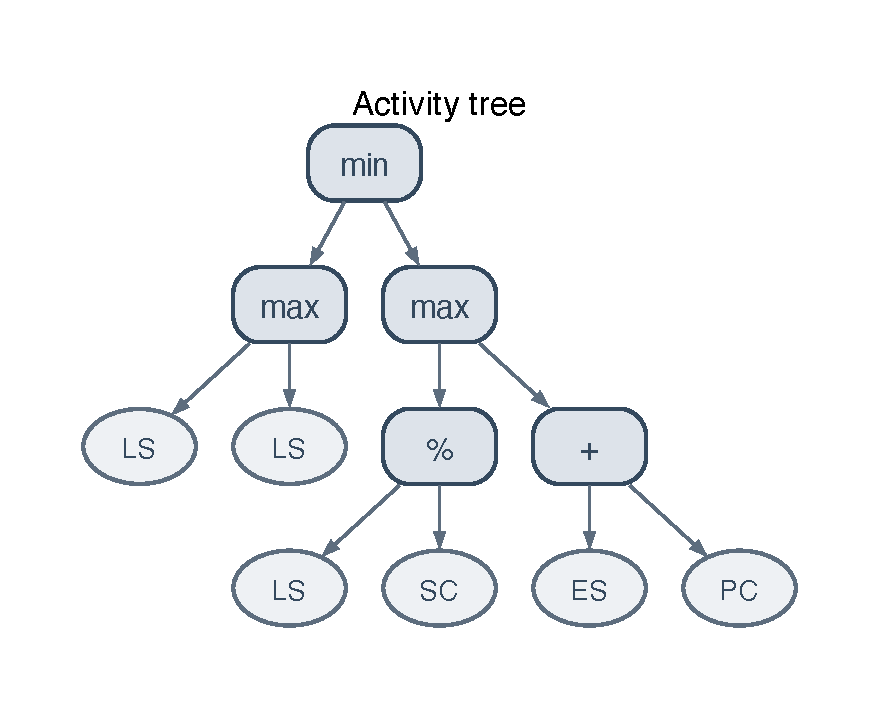
\includegraphics[width=0.5\textwidth]{img/generated/gp_tree_localsearch_activity.pdf}\\[1.5ex]
  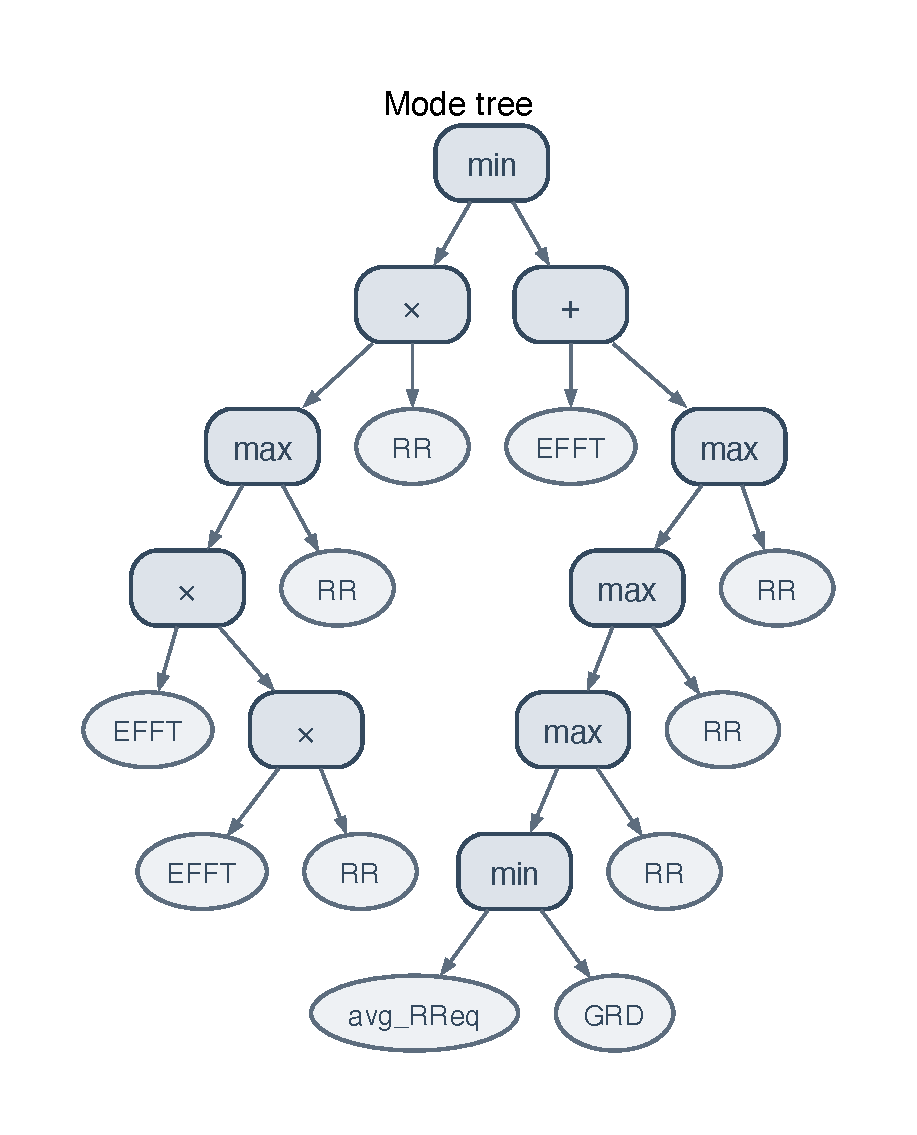
\includegraphics[width=0.78\textwidth]{img/generated/gp_tree_localsearch_mode.pdf}
  \caption[Evolved activity and mode tree under critical-path local
  search]{\changedC{Compact evolved trees under critical-path local search
  (serial/mode-first, MMLIB100). The two panels are from two champions of
  that cell, each chosen as the most compact interpretable example of its
  tree type, since the smallest single individual's activity tree collapses
  to the bare minimum-LST terminal \texttt{LS}. Top: an activity tree,
  $\min(\texttt{LS}, \max(\texttt{LS}/\texttt{SC},
  \texttt{ES} + \texttt{PC}))$, a minimum-latest-start-time rule that lets
  activities with several immediate successors move forward (the duplicated
  $\max(\texttt{LS}, \texttt{LS})$ \changedD{simplifies to} \texttt{LS}).
  Bottom: a mode tree, which prefers modes that finish early (\texttt{EFFT})
  and request few resource types (\texttt{RR}).} \changedB{Colours and
  operators as in Figure~\ref{fig:nr-evolved-tree}; the standard baseline
  terminal set is used throughout.}}
  \label{fig:localsearch-evolved-tree}
\end{figure}

\subsection{Comprehensive evaluation of NR terminals}
\label{subsec:nr-eval}

NR terminals (defined in full in Section~\ref{subsec:nr-terminals-definition}:
\texttt{NR\_STOCK\_RATIO}, \texttt{NR\_MODE\_DEMAND\_RATIO}, and
\texttt{NR\_BUDGET\_PRESSURE}) close the baseline terminal set's one
significant blind spot, visibility into non-renewable resource state, and
are evaluated here for the first time at full statistical power. Because
these terminals are only meaningful on instances that still carry their
non-renewable resources, this condition is evaluated on NR-preserving
instances rather than \changedC{the renewable-only-converted set of the
baseline paper (Tian et al.~\cite{Tian2024GPHH})} used
everywhere else in this chapter, against \texttt{baseline\_nr}, the
unmodified baseline algorithm run on the same NR-preserving instances, as
its matched control. The two conditions are directly comparable to each
other, but their ARD\% figures are \emph{not} comparable in magnitude to
the baseline/lexicase/local-search figures above, because the CPM lower
bound used for normalisation ignores resource constraints entirely
(Section~\ref{sec:eval-metrics}), and is consequently far looser, relative
to true achievable makespan, on NR-preserving instances than on the
renewable-only-converted ones. \changedC{Because infeasible schedules have
no meaningful makespan, every ARD\% figure in the tables of this section
(as everywhere in this chapter,
Section~\ref{subsec:statistical-methodology}) is a mean over the instances
a rule scheduled feasibly; the instances it failed on are not
\changedD{included in} the mean but reported separately, as the feasibility rate in
Table~\ref{tab:nr-descriptive-stats} for MMLIB50 and
Table~\ref{tab:nr-descriptive-stats-mmlib100} for MMLIB100. This matters here more than in the
two comparisons above, where feasibility was uniformly $1.00$: when
conditions differ in feasibility, their feasible-only means are computed
over different instance subsets, which is why the two metrics must always
be read together.}

\begin{table}[htbp]
  \centering
  \small
  \shrinktofit{%
  \caption[NR terminals vs.\ baseline on MMLIB50]{Mean ARD\% (\%),
  \texttt{baseline\_nr} vs.\ NR terminals, MMLIB50 (NR-preserving
  instances), $n=30$ seeds per cell.}
  \label{tab:nr-vs-baseline-mmlib50}
  \begin{tabular}{llrrrr}
    \toprule
    \textbf{SGS} & \textbf{Strategy} & \textbf{\texttt{baseline\_nr} (test)} & \textbf{NR terminals (test)} & \textbf{\texttt{baseline\_nr} (train)} & \textbf{NR terminals (train)} \\
    \midrule
    Parallel & AF & 140.92 & 121.74\,\ArrBetter & 121.89 & 102.99\,\ArrBetter \\
    Parallel & MF & 143.14 & 124.85\,\ArrBetter & 123.11 & 105.66\,\ArrBetter \\
    Parallel & S  & 144.86 & 129.27\,\ArrBetter & 123.27 & 108.49\,\ArrBetter \\
    Serial   & AF & 140.36 & 109.23\,\ArrBetter & 120.86 &  88.10\,\ArrBetter \\
    Serial   & MF & 139.05 & 113.54\,\ArrBetter & 119.86 &  90.13\,\ArrBetter \\
    Serial   & S  & 144.34 & 110.37\,\ArrBetter & 123.71 &  87.41\,\ArrBetter \\
    \bottomrule
  \end{tabular}%
  }
\end{table}

\begin{table}[htbp]
  \centering
  \small
  \shrinktofit{%
  \caption[Descriptive statistics: NR terminals vs.\ baseline]{Standard
  deviation and, unlike the two comparisons above, a clearly
  \emph{non-uniform} feasibility rate: NR terminals raise held-out test
  feasibility from roughly 68--70\% to roughly 82--86\% across every cell,
  in addition to improving the feasible-only mean ARD\% reported in
  Table~\ref{tab:nr-vs-baseline-mmlib50}.}
  \label{tab:nr-descriptive-stats}
  \begin{tabular}{lllrrrr}
    \toprule
    \textbf{SGS} & \textbf{Strategy} & \textbf{Split} & \textbf{\texttt{baseline\_nr} std} & \textbf{NR std} & \textbf{\texttt{baseline\_nr} feas.} & \textbf{NR feas.} \\
    \midrule
    Parallel & AF & Train &  8.60 & 8.61 & 0.93 & 1.00 \\
    Parallel & AF & Test  & 14.84 & 11.69 & 0.69 & 0.85 \\
    Parallel & MF & Train &  6.49 & 5.67 & 0.93 & 1.00 \\
    Parallel & MF & Test  & 10.98 & 9.77 & 0.69 & 0.82 \\
    Parallel & S  & Train &  5.74 & 4.70 & 0.94 & 1.00 \\
    Parallel & S  & Test  &  8.15 & 8.34 & 0.68 & 0.82 \\
    Serial   & AF & Train &  4.76 & 5.47 & 1.00 & 1.00 \\
    Serial   & AF & Test  &  6.05 & 9.77 & 0.69 & 0.82 \\
    Serial   & MF & Train &  7.59 & 6.88 & 1.00 & 1.00 \\
    Serial   & MF & Test  & 13.25 & 8.96 & 0.68 & 0.83 \\
    Serial   & S  & Train &  4.71 & 7.54 & 0.98 & 1.00 \\
    Serial   & S  & Test  &  6.57 & 10.89 & 0.70 & 0.86 \\
    \bottomrule
  \end{tabular}%
  }
\end{table}

\begin{table}[htbp]
  \centering
  \small
  \shrinktofit{%
  \caption[Statistical significance: NR terminals vs.\ baseline]{Two-sided
  paired Wilcoxon signed-rank test and matched rank-biserial effect size
  $r$, NR terminals vs.\ \texttt{baseline\_nr}, MMLIB50, $n=30$ per cell.
  Every one of the twelve train/test comparisons is significant at
  $p<0.0001$ with a large effect size ($r \geq 0.815$).}
  \label{tab:nr-significance}
  \begin{tabular}{lllrrl}
    \toprule
    \textbf{SGS} & \textbf{Strategy} & \textbf{Split} & \textbf{$p$} & \textbf{$r$} & \textbf{Verdict} \\
    \midrule
    Parallel & AF & Train & $<0.0001$ & $+0.923$ & Significant, favours NR terminals \\
    Parallel & AF & Test  & $<0.0001$ & $+0.815$ & Significant, favours NR terminals \\
    Parallel & MF & Train & $<0.0001$ & $+0.987$ & Significant, favours NR terminals \\
    Parallel & MF & Test  & $<0.0001$ & $+0.927$ & Significant, favours NR terminals \\
    Parallel & S  & Train & $<0.0001$ & $+0.948$ & Significant, favours NR terminals \\
    Parallel & S  & Test  & $<0.0001$ & $+0.948$ & Significant, favours NR terminals \\
    Serial   & AF & Train & $<0.0001$ & $+1.000$ & Significant, favours NR terminals \\
    Serial   & AF & Test  & $<0.0001$ & $+1.000$ & Significant, favours NR terminals \\
    Serial   & MF & Train & $<0.0001$ & $+1.000$ & Significant, favours NR terminals \\
    Serial   & MF & Test  & $<0.0001$ & $+0.966$ & Significant, favours NR terminals \\
    Serial   & S  & Train & $<0.0001$ & $+1.000$ & Significant, favours NR terminals \\
    Serial   & S  & Test  & $<0.0001$ & $+1.000$ & Significant, favours NR terminals \\
    \bottomrule
  \end{tabular}%
  }
\end{table}

\begin{figure}[htbp]
  \centering
  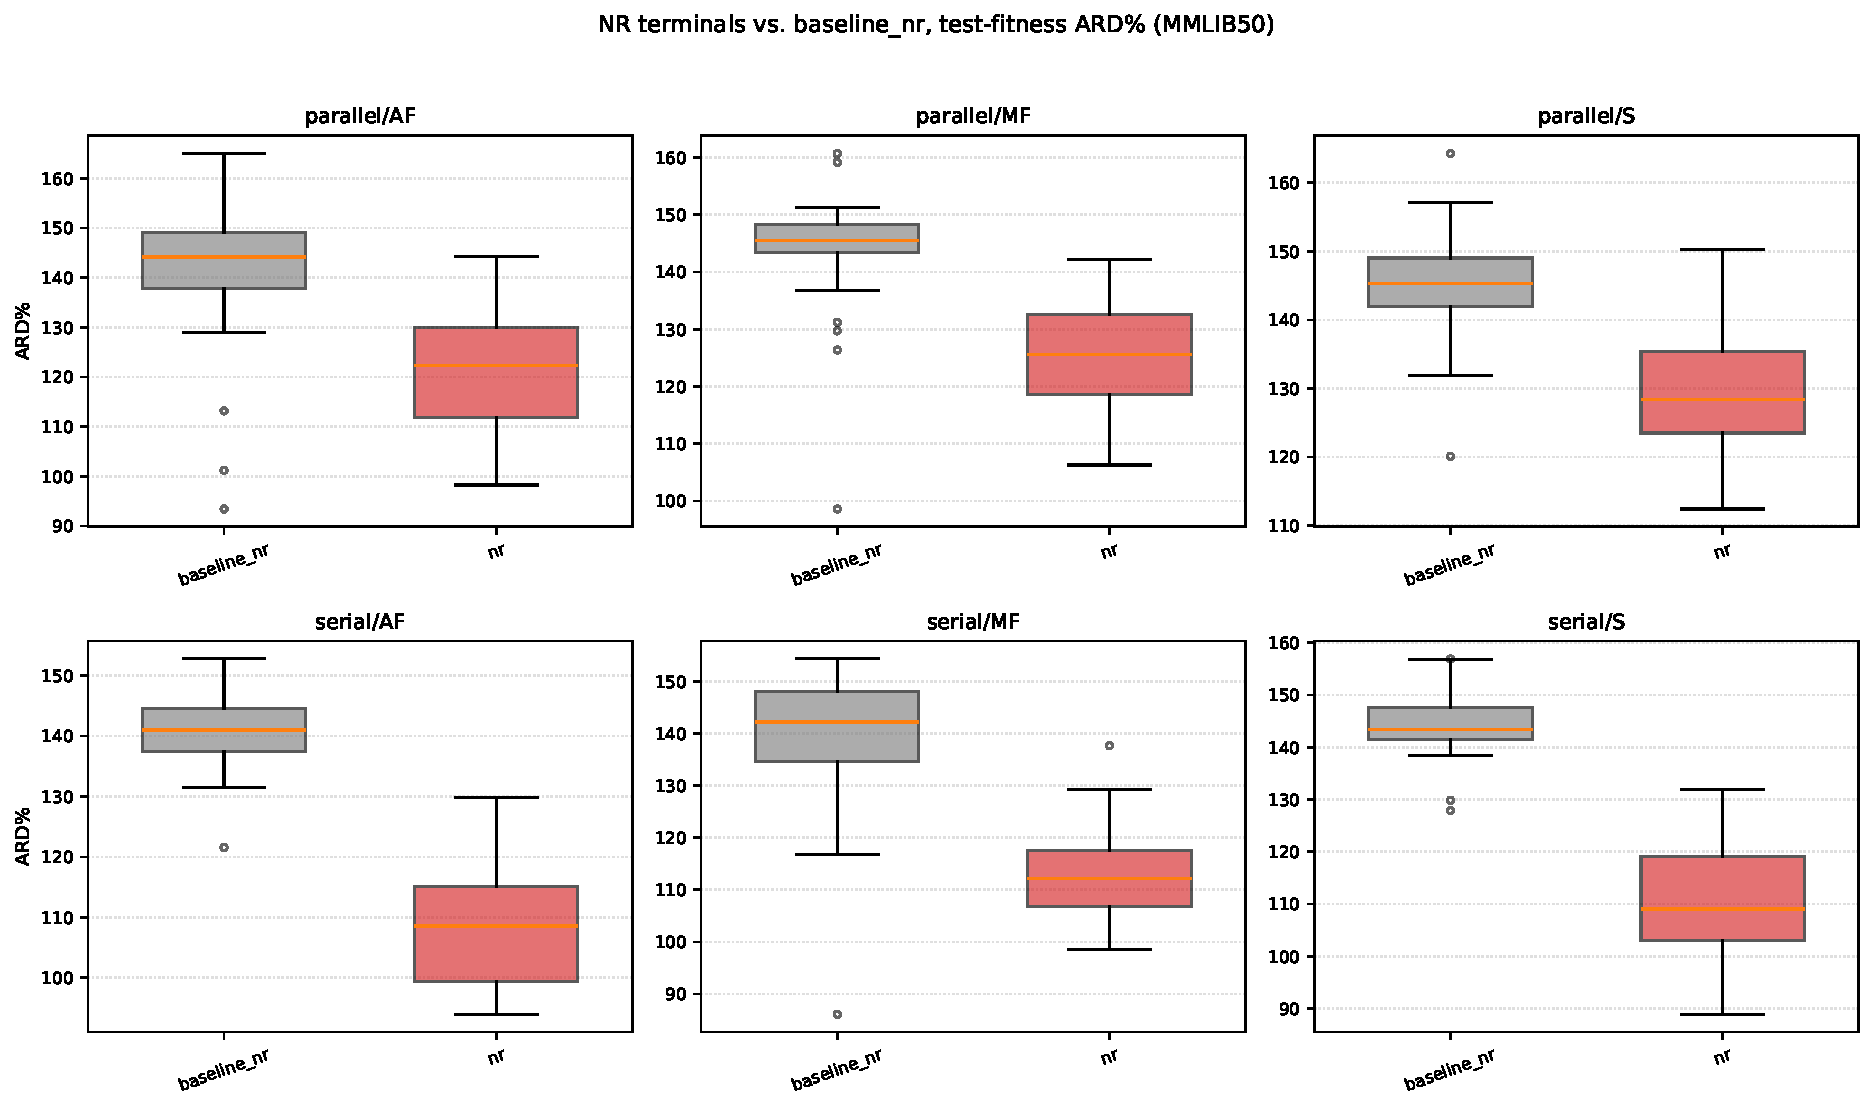
\includegraphics[width=0.95\textwidth]{img/generated/nr_boxplot_mmlib50.pdf}
  \caption{Distribution of test-fitness ARD\%, NR terminals vs.\
  \texttt{baseline\_nr}, MMLIB50 NR-preserving instances, one panel per
  (SGS, strategy) cell, 30 seeds per box. Note the much larger ARD\% scale
  than Figures~\ref{fig:lexicase-boxplot}/\ref{fig:localsearch-boxplot},
  a consequence of the looser CPM lower bound on NR-preserving instances
  (Section~\ref{subsec:threats-construct}), not of the algorithms
  themselves.}
  \label{fig:nr-boxplot}
\end{figure}

\begin{figure}[htbp]
  \centering
  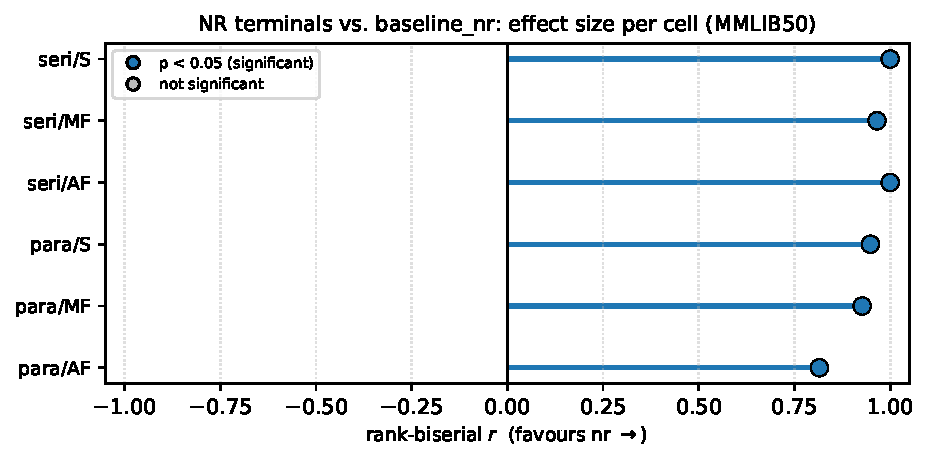
\includegraphics[width=0.85\textwidth]{img/generated/nr_effectsize_mmlib50.pdf}
  \caption[Effect-size summary, NR terminals vs.\ baseline\_nr]{Effect-size
  summary, NR terminals vs.\ \texttt{baseline\_nr}, MMLIB50: matched
  rank-biserial correlation $r$ per (SGS, strategy) cell (positive favours
  NR terminals), filled markers denote $p<0.05$; every cell is significant
  and favourable, see Figure~\ref{fig:lexicase-cd}'s caption for why a
  per-cell effect-size plot, not a Nemenyi CD diagram, is used for this
  two-condition comparison.}
  \label{fig:nr-cd}
\end{figure}

\begin{table}[htbp]
  \centering
  \small
  \shrinktofit{%
  \caption[NR terminals vs.\ baseline on MMLIB100]{Mean ARD\% (\%),
  \texttt{baseline\_nr} vs.\ NR terminals, MMLIB100 (NR-preserving
  instances, scalability validation), $n=30$ seeds per cell.
  \changedC{Each mean is taken only over the instances a rule scheduled
  feasibly; infeasible instances receive no penalty value and are instead
  reported separately as the feasibility rate in
  Table~\ref{tab:nr-descriptive-stats-mmlib100}. Because the two
  conditions differ in feasibility, their means cover different instance
  subsets, so the two tables must be read together.}}
  \label{tab:nr-vs-baseline-mmlib100}
  \begin{tabular}{llrrrr}
    \toprule
    \textbf{SGS} & \textbf{Strategy} & \textbf{\texttt{baseline\_nr} (test)} & \textbf{NR terminals (test)} & \textbf{\texttt{baseline\_nr} (train)} & \textbf{NR terminals (train)} \\
    \midrule
    Parallel & AF & 114.37 & 113.77\,\ArrBetter & 107.46 & 108.28\,\ArrWorse \\
    Parallel & MF & 113.68 & 114.34\,\ArrWorse & 106.25 & 108.46\,\ArrWorse \\
    Parallel & S  & 124.88 & 110.56\,\ArrBetter & 115.22 & 105.15\,\ArrBetter \\
    Serial   & AF & 118.46 &  90.07\,\ArrBetter & 110.18 &  83.68\,\ArrBetter \\
    Serial   & MF & 116.98 &  89.85\,\ArrBetter & 108.51 &  83.45\,\ArrBetter \\
    Serial   & S  & 124.49 &  83.16\,\ArrBetter & 116.33 &  78.59\,\ArrBetter \\
    \bottomrule
  \end{tabular}%
  }
\end{table}

\begin{table}[htbp]
  \centering
  \small
  \shrinktofit{%
  \caption[Descriptive statistics: NR terminals vs.\ baseline, MMLIB100]{\changedC{Standard
  deviation and feasibility rate accompanying
  Table~\ref{tab:nr-vs-baseline-mmlib100}, MMLIB100. The feasibility gain
  replicates at the larger scale in every cell, though from a higher
  baseline and by a smaller margin than on MMLIB50: held-out test
  feasibility rises from roughly 75--88\% under \texttt{baseline\_nr} to
  roughly 87--93\% under NR terminals.}}
  \label{tab:nr-descriptive-stats-mmlib100}
  \begin{tabular}{lllrrrr}
    \toprule
    \textbf{SGS} & \textbf{Strategy} & \textbf{Split} & \textbf{\texttt{baseline\_nr} std} & \textbf{NR std} & \textbf{\texttt{baseline\_nr} feas.} & \textbf{NR feas.} \\
    \midrule
    Parallel & AF & Train &  8.66 &  6.43 & 0.91 & 0.99 \\
    Parallel & AF & Test  & 11.42 &  8.17 & 0.75 & 0.89 \\
    Parallel & MF & Train & 11.76 &  7.82 & 0.91 & 0.98 \\
    Parallel & MF & Test  & 14.32 &  8.27 & 0.75 & 0.87 \\
    Parallel & S  & Train & 11.52 &  7.10 & 0.91 & 1.00 \\
    Parallel & S  & Test  & 14.97 &  9.77 & 0.78 & 0.88 \\
    Serial   & AF & Train &  9.16 &  4.52 & 0.99 & 1.00 \\
    Serial   & AF & Test  & 11.43 &  4.64 & 0.83 & 0.93 \\
    Serial   & MF & Train &  8.12 &  4.02 & 1.00 & 1.00 \\
    Serial   & MF & Test  &  9.98 &  5.04 & 0.85 & 0.90 \\
    Serial   & S  & Train &  8.21 & 10.31 & 0.98 & 1.00 \\
    Serial   & S  & Test  & 11.00 & 12.89 & 0.88 & 0.91 \\
    \bottomrule
  \end{tabular}%
  }
\end{table}

\begin{table}[htbp]
  \centering
  \small
  \shrinktofit{%
  \caption[Statistical significance: NR terminals vs.\ baseline, MMLIB100]{Two-sided
  paired Wilcoxon signed-rank test and matched rank-biserial effect size
  $r$, NR terminals vs.\ \texttt{baseline\_nr}, MMLIB100.}
  \label{tab:nr-significance-mmlib100}
  \begin{tabular}{lllrrl}
    \toprule
    \textbf{SGS} & \textbf{Strategy} & \textbf{Split} & \textbf{$p$} & \textbf{$r$} & \textbf{Verdict} \\
    \midrule
    Parallel & AF & Train & 0.6408 & $-0.101$ & Not significant \\
    Parallel & AF & Test  & 0.7151 & $+0.080$ & Not significant \\
    Parallel & MF & Train & 0.4400 & $-0.166$ & Not significant \\
    Parallel & MF & Test  & 0.7766 & $-0.062$ & Not significant \\
    Parallel & S  & Train & 0.0005 & $+0.695$ & Significant, favours NR terminals \\
    Parallel & S  & Test  & 0.0002 & $+0.742$ & Significant, favours NR terminals \\
    Serial   & AF & Train & $<0.0001$ & $+1.000$ & Significant, favours NR terminals \\
    Serial   & AF & Test  & $<0.0001$ & $+1.000$ & Significant, favours NR terminals \\
    Serial   & MF & Train & $<0.0001$ & $+1.000$ & Significant, favours NR terminals \\
    Serial   & MF & Test  & $<0.0001$ & $+0.996$ & Significant, favours NR terminals \\
    Serial   & S  & Train & $<0.0001$ & $+1.000$ & Significant, favours NR terminals \\
    Serial   & S  & Test  & $<0.0001$ & $+1.000$ & Significant, favours NR terminals \\
    \bottomrule
  \end{tabular}%
  }
\end{table}

\begin{figure}[htbp]
  \centering
  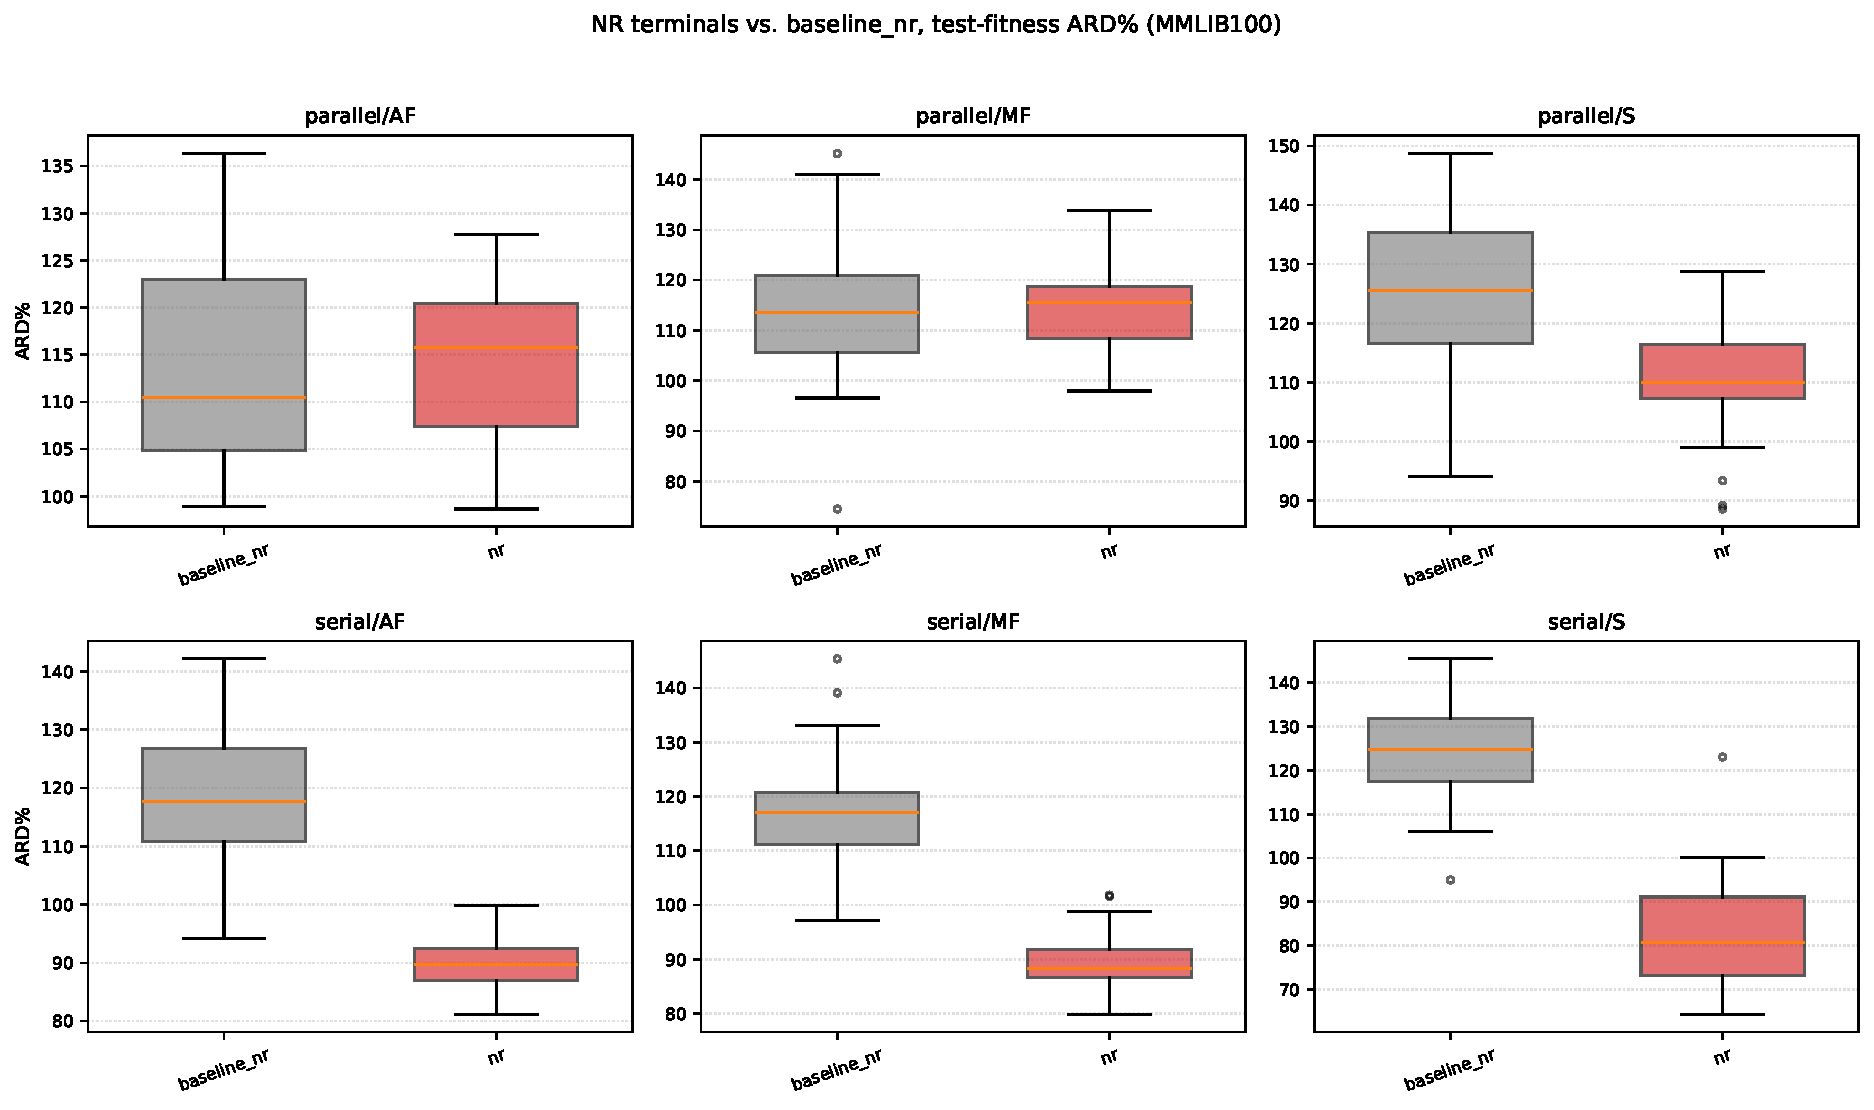
\includegraphics[width=0.95\textwidth]{img/generated/nr_boxplot_mmlib100.pdf}
  \caption{Distribution of test-fitness ARD\%, NR terminals vs.\
  \texttt{baseline\_nr}, MMLIB100, same layout as Figure~\ref{fig:nr-boxplot}.
  Note the visibly overlapping boxes in the two parallel/AF and parallel/MF
  panels, contrasting with the clear separation in the other four.}
  \label{fig:nr-boxplot-mmlib100}
\end{figure}

\begin{figure}[htbp]
  \centering
  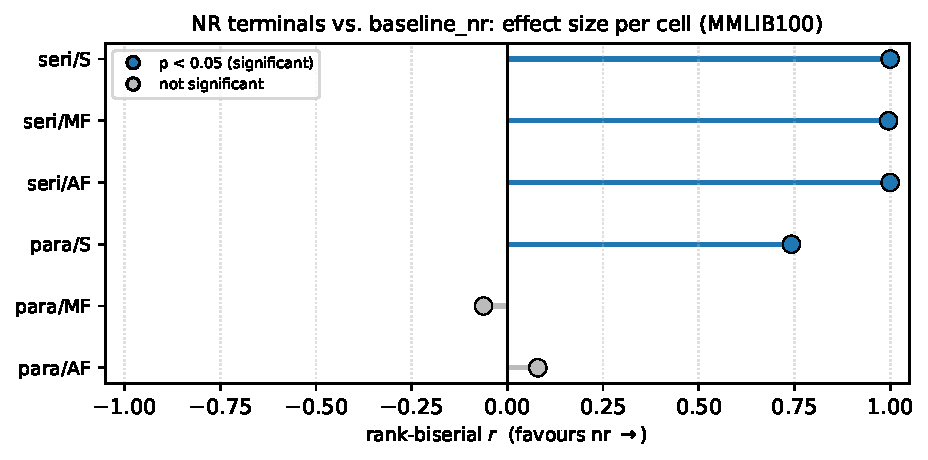
\includegraphics[width=0.85\textwidth]{img/generated/nr_effectsize_mmlib100.pdf}
  \caption[Effect-size summary, NR terminals vs.\ baseline\_nr, MMLIB100]{Effect-size
  summary, NR terminals vs.\ \texttt{baseline\_nr}, MMLIB100: four cells
  remain strongly favourable and significant, while parallel/AF and
  parallel/MF collapse toward zero, the visual counterpart of
  Table~\ref{tab:nr-significance-mmlib100}.}
  \label{fig:nr-cd-mmlib100}
\end{figure}

On \textbf{MMLIB50}, this is, by a wide margin, the most robust result in
this chapter. Every one of the twelve train/test comparisons across all six
(SGS, strategy) cells reaches significance at $p<0.0001$ with a large
effect size ($r \geq 0.815$), and, unlike either selection or local search,
the effect is stable in both sign and magnitude across every decoding
scheme and every GP decision strategy: there is no SGS-dependent reversal
here of the kind seen in Sections~\ref{subsec:lexicase-eval}
and~\ref{subsec:localsearch-eval}. \changedC{The mechanism behind this is
straightforward:}
without any NR signal, the baseline can only avoid exhausting the project's
non-renewable budget by chance, and Table~\ref{tab:nr-descriptive-stats}
shows this directly in the feasibility rate, not just the mean. Held-out
test feasibility rises from roughly 68--70\% under \texttt{baseline\_nr} to
roughly 82--86\% under NR terminals in every single cell, meaning the
improvement is not solely a matter of NR terminals producing modestly
better schedules on the instances both conditions could already solve; it
is also solving a meaningfully larger share of instances that the baseline
could not solve at all. \changedB{One qualification to this feasibility
gain is established later: re-evaluated on the complete 108-class test
set, it proves largely confined to the instance classes seen during
training, while the schedule-quality advantage carries over in full
(Section~\ref{subsec:full108}).}

\textbf{Scalability validation.} Table~\ref{tab:nr-significance-mmlib100}
qualifies \changed{these results} in a specific and informative way rather than
simply confirming them. Four of the six MMLIB100 cells, both serial/AF,
serial/MF, serial/S and, notably, parallel/S, replicate MMLIB50's result
almost exactly, large, significant effects on both train and test fitness
($r=0.695$--$1.000$). The remaining two cells, parallel/AF and
parallel/MF, do not: at MMLIB100 scale neither the training-fitness nor the
test-fitness advantage reaches significance ($p=0.44$--$0.78$, $|r|\leq
0.17$), a marked change from MMLIB50's own parallel/AF and parallel/MF rows,
which were both significant there ($r=0.815$--$0.987$). This is a genuine,
specific scale-dependence, not a uniform weakening: NR terminals' benefit
is confirmed as robust to instance size under serial SGS (all three
strategies) and under parallel/simultaneous, but does not clearly survive
scaling from MMLIB50 to MMLIB100 under parallel/activity-first or
parallel/mode-first. \changedC{The feasibility side of the result is more
uniform: Table~\ref{tab:nr-descriptive-stats-mmlib100} shows NR terminals
raising the held-out feasibility rate in all six cells at MMLIB100,
including the two whose fitness advantage vanishes, so what fails to
replicate in parallel/AF and parallel/MF is the schedule-quality gain,
not the ability to find feasible schedules. Read together with the
feasible-only convention stated above, those two cells' near-equal mean
ARD\% is if anything conservative: the NR condition achieves it while
feasibly scheduling a larger, and therefore presumably harder, share of
the test instances.}

The cells that fail share a specific structural property the cells that
succeed do not, which points to a concrete mechanism rather than a vague
``more complexity'' explanation. Activity-first and mode-first both split
the decision into two independently evolved trees (Section~\ref{subsec:individual-representation}):
the activity tree sees \texttt{NR\_STOCK\_RATIO}/\texttt{NR\_BUDGET\_PRESSURE},
the mode tree sees \texttt{NR\_MODE\_DEMAND\_RATIO}, and the two trees can
only coordinate an NR-aware trade-off implicitly, through the shared
fitness signal, never within a single expression. Simultaneous mode uses
one integrated tree that scores each (activity, mode) pair jointly, so it
can encode a rule like ``favour this activity only if some mode of it
keeps NR demand low'' directly, with both signals visible to the same
expression at the same time. Parallel SGS is precisely the decoding scheme
that stresses the split-tree architecture's coordination gap: unlike serial
SGS, which commits one activity/mode pair at a time and updates the
remaining NR budget immediately afterwards, parallel SGS advances a single
global clock and can commit \emph{several} activities' mode choices within
the same time step, all drawing against the same NR budget before it is
next updated. Coordinating that many simultaneous, mutually competing
NR-relevant choices correctly is exactly the kind of joint reasoning an
integrated tree can express directly and two decoupled trees can only
approximate through indirect selection pressure. MMLIB100's larger
instances make this \changed{harder}:
more activities per instance means more candidate activities are typically
eligible, and hence more simultaneous mode decisions are competing for the
same shrinking NR budget within a single parallel-SGS time step, than on
MMLIB50's smaller instances. Simultaneous mode is insulated from this
because it never had to solve the coordination problem in the first place;
serial SGS is insulated because it never presents the simultaneous
contention that makes the coordination problem hard. Activity-first and
mode-first under parallel SGS are the one combination exposed to both the
coordination gap and \changed{the scale at which it becomes decisive. This
account is consistent with} Section~\ref{subsec:localsearch-eval}'s
observation that parallel SGS's simultaneous commits leave more exploitable
structure in the resulting schedule than serial SGS's one-at-a-time
construction: the same architectural difference between the two decoding
schemes that gives local search more to work with under parallel SGS is
what gives a split-tree NR rule more simultaneous contention to fail to
coordinate. Directly testing this account, for instance by comparing how
often activity-first/mode-first's two trees make internally consistent
NR-aware choices within the same parallel-SGS time step versus how often
they contradict each other, is left as future work
(Section~\ref{sec:future-work}). Even with this qualification, NR terminals
remain this thesis's strongest and most broadly replicated result: unlike
lexicase (which weakens further at MMLIB100) or local search (whose one
significant MMLIB50 win disappears entirely), four of NR terminals' six
cells replicate cleanly, and none reverses direction.

Two further caveats qualify, without undermining, this result. First,
because \texttt{nr} necessarily runs on a different instance set
(NR-preserving) than \texttt{baseline}, \texttt{lexicase}, and
\texttt{local\_search} above, this comparison cannot be \changedD{included in} the
same six-cell, four-condition ranking used in
Section~\ref{subsec:final-comparison}\changed{; it is therefore reported
here as its own, self-contained result}. Second,
generalisation to instances harder than MMLIB100, in particular MMLIB+'s
tighter NR budgets, is not established by this section; a separate,
smaller-scale, instance-matched study (referenced in the repository's own
experiment log) found the same direction of effect on MMLIB+ but with
markedly higher test infeasibility for both conditions, a question
Section~\ref{sec:future-work} returns to.

\changedB{Beyond the aggregate statistics, it is worth looking at what the
NR-aware GPHH actually evolves. Figure~\ref{fig:nr-evolved-tree} shows a
compact evolved rule pair from the serial/activity-first cell, chosen as the
smallest run (by total node count) that still recruits the non-renewable
terminals in both trees, so the mechanism is legible without the visual
clutter of a larger individual. Both trees reference the new terminals
without any prompting: the activity tree gates its priority on
\texttt{NR\_STOCK\_RATIO}, so activities are ordered partly by how much of
the non-renewable budget remains, while the mode tree is dominated by
\texttt{NR\_MODE\_DEMAND\_RATIO}\changedC{, penalising modes whose
non-renewable demand is high relative to what is left. The evolved
individual references that terminal four times, but two of the four form a
subtree dividing it by itself, which under protected division is the
constant $1$, a typical piece of functionally neutral code that GP trees
accumulate;
Figure~\ref{fig:nr-evolved-tree} omits one of that subtree's two identical
operands for legibility, so the terminal is drawn three times there. The
two \changedD{remaining} references each divide \texttt{NR\_MODE\_DEMAND\_RATIO} by
the resource-count terminal \texttt{RR}. This is direct evidence that the
improvement reported above comes from the rule actually using the new
information rather than from some incidental side effect of enlarging the
terminal set:} given visibility into the non-renewable state,
evolution places those terminals at \changedD{important} positions in the rule
rather than leaving them as unused vocabulary.}
\changedC{Nor is this recruitment specific to the displayed pair: across
all of the \texttt{nr} condition's champions (the champion-wide analysis
of Section~\ref{subsec:localsearch-eval}),
\texttt{NR\_MODE\_DEMAND\_RATIO} is recruited by every single mode and
integrated tree ($100\%$ under both SGS), \texttt{NR\_STOCK\_RATIO}
appears in $81\%$ of the parallel activity trees, and
\texttt{NR\_BUDGET\_PRESSURE} in about three quarters of the serial
ones, so the new terminals are, population-wide, among the most
recruited vocabulary the rules have.}

\begin{figure}[htbp]
  \centering
  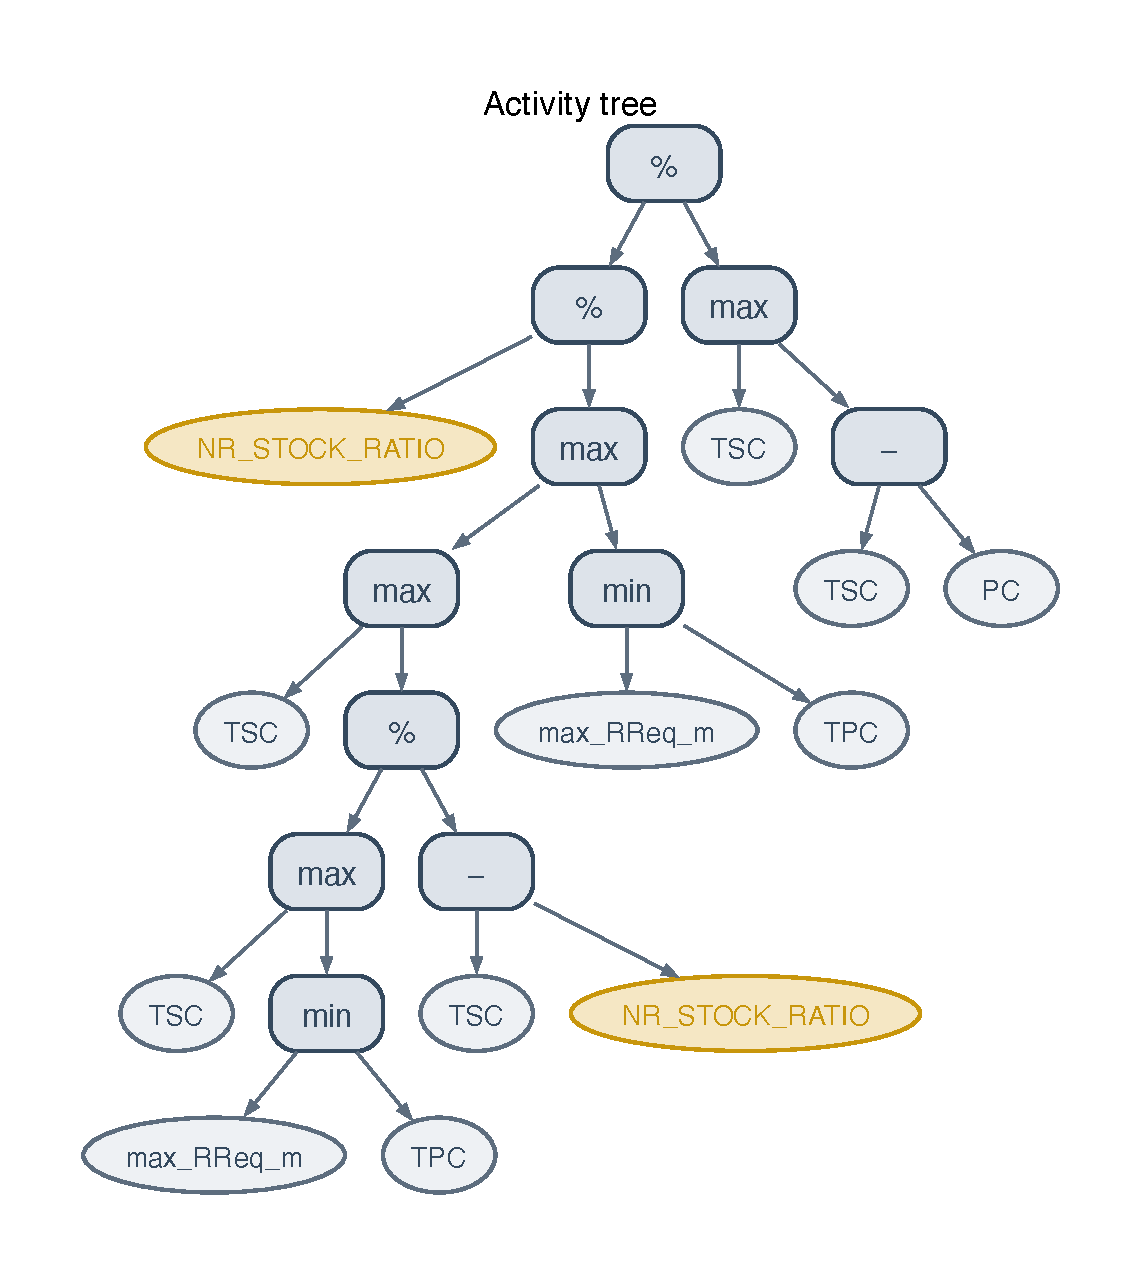
\includegraphics[width=0.62\textwidth]{img/generated/gp_tree_evolved_activity.pdf}\\[1.5ex]
  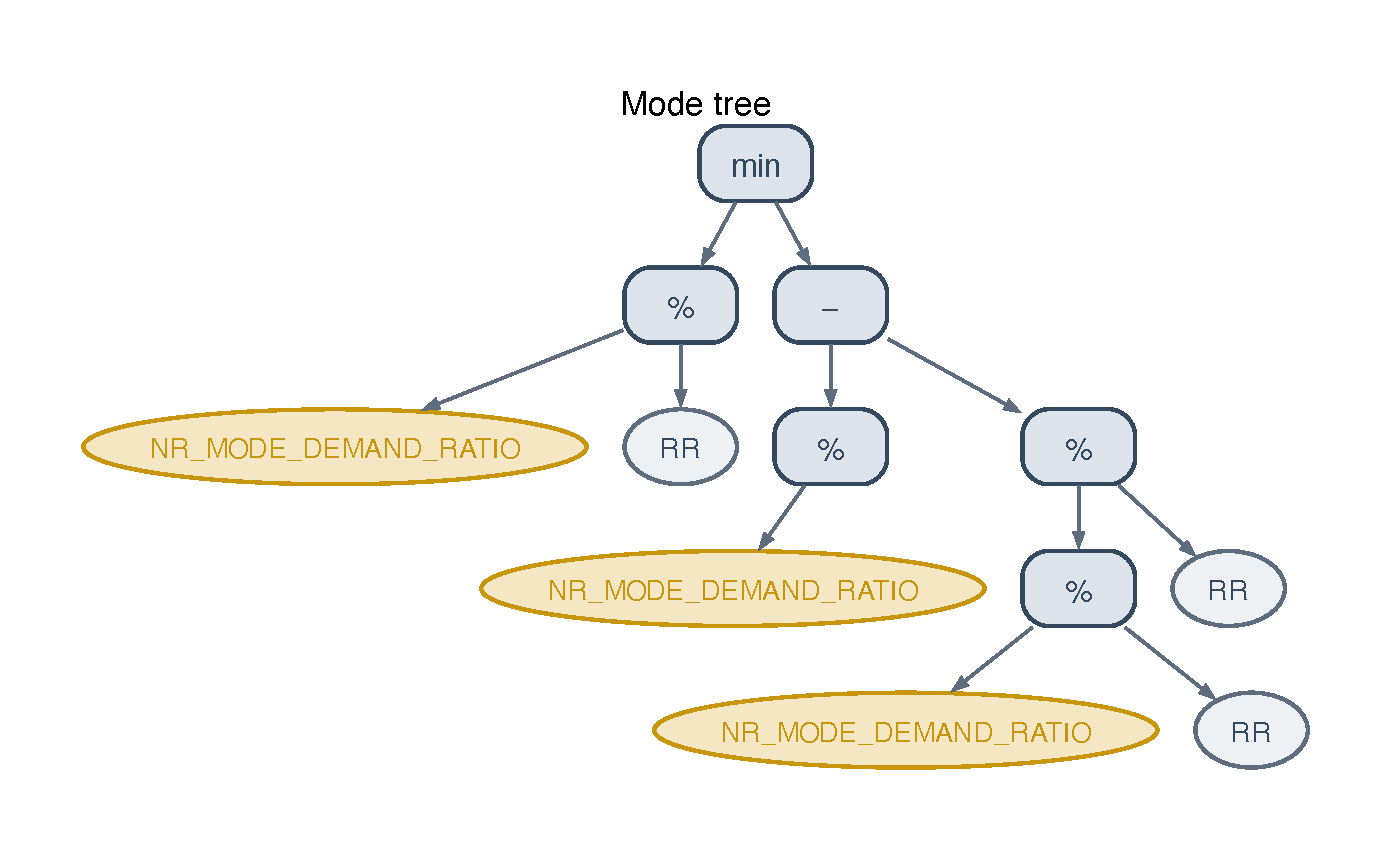
\includegraphics[width=0.98\textwidth]{img/generated/gp_tree_evolved_mode.pdf}
  \caption[Evolved NR-aware rule pair]{\changedB{A compact evolved NR-aware
  rule pair (serial/activity-first, MMLIB50), selected as the smallest
  individual that recruits the non-renewable terminals in both trees.
  Top: the activity tree, which selects the next activity to schedule.
  Bottom: the mode tree, which selects its execution mode. Operator nodes are
  blue; ordinary terminals are grey; the non-renewable terminals contributed
  by this work (\texttt{NR\_STOCK\_RATIO},
  \texttt{NR\_MODE\_DEMAND\_RATIO}) are highlighted in gold. The GP function
  set is $\{+, -, \times, \%, \min, \max\}$, where $\%$ denotes protected
  division.}}
  \label{fig:nr-evolved-tree}
\end{figure}

\section{Benchmark evaluation and baseline comparison}
\label{sec:benchmark-comparison}

Sections~\ref{subsec:lexicase-eval} through~\ref{subsec:nr-eval} each
compared one candidate modification against its own matched baseline in
isolation, which answers whether that specific modification helps but not
how the modifications compare against one another or which, if any, would
be the single configuration worth recommending. This section closes that
gap: it ranks baseline, lexicase, local search, and hybrid jointly on the
same six-cell grid, reports NR terminals' result alongside for qualitative
reference, and summarises what the comprehensive stage as a whole,
MMLIB50's complete grid together with MMLIB100's scalability check,
supports as this thesis's final, evidence-based verdict.

\subsection{Final comparison and summary}
\label{subsec:final-comparison}

\changed{The four jointly ranked conditions are baseline, lexicase, local
search, and hybrid (lexicase selection and local search applied together),
compared with the average-rank and Friedman methodology of
Section~\ref{subsec:statistical-methodology}.}

\begin{table}[htbp]
  \centering
  \small
  \shrinktofit{%
  \caption[Method rankings]{Average rank (1 = best, 4 = worst) across the
  six (SGS, strategy) cells, MMLIB50, test and train fitness. The test-rank
  Friedman test is significant ($\chi^2 = 10.20$, $p = 0.0169$, 6 blocks, 4
  conditions); the train-rank Friedman test is not ($\chi^2 = 0.20$,
  $p = 0.978$).}
  \label{tab:method-rankings}
  \begin{tabular}{lrrrr}
    \toprule
    \textbf{Condition} & \textbf{Avg.\ rank (test)} & \textbf{Avg.\ rank (train)} \\
    \midrule
    Local search & 1.50 & 2.67 \\
    Baseline     & 2.33 & 2.50 \\
    Lexicase     & 2.33 & 2.50 \\
    Hybrid       & 3.83 & 2.33 \\
    \bottomrule
  \end{tabular}%
  }
\end{table}

\begin{table}[htbp]
  \centering
  \small
  \shrinktofit{%
  \caption[Final comparison on MMLIB50]{Final side-by-side comparison of
  all four jointly ranked conditions, mean test-fitness ARD\% (\%),
  MMLIB50, the same six rows underlying Table~\ref{tab:method-rankings}'s
  ranks. *NR terminals' own result is appended for qualitative reference
  only: it runs on NR-preserving instances against \texttt{baseline\_nr},
  not the renewable-only-converted instances the other four columns share,
  so it is \emph{not} on the same ARD\% scale and must not be compared
  numerically against the other columns (Section~\ref{subsec:nr-eval}).}
  \label{tab:final-comparison-mmlib50}
  \begin{tabular}{llrrrrr}
    \toprule
    \textbf{SGS} & \textbf{Strategy} & \textbf{Baseline} & \textbf{Lexicase} & \textbf{Local search} & \textbf{Hybrid} & \textbf{NR terminals*} \\
    \midrule
    Parallel & AF & 35.77 & 34.36\,\ArrBetter & 33.64\,\ArrBetter & 34.51\,\ArrBetter & 121.74 \\
    Parallel & MF & 35.78 & 35.50\,\ArrBetter & 35.57\,\ArrBetter & 36.08\,\ArrWorse & 124.85 \\
    Parallel & S  & 30.43 & 30.08\,\ArrBetter & 29.79\,\ArrBetter & 30.72\,\ArrWorse & 129.27 \\
    Serial   & AF & 17.81 & 18.33\,\ArrWorse & 18.24\,\ArrWorse & 18.56\,\ArrWorse & 109.23 \\
    Serial   & MF & 17.89 & 18.52\,\ArrWorse & 18.37\,\ArrWorse & 19.08\,\ArrWorse & 113.54 \\
    Serial   & S  & 18.08 & 18.41\,\ArrWorse & 17.77\,\ArrBetter & 18.43\,\ArrWorse & 110.37 \\
    \bottomrule
  \end{tabular}%
  }
\end{table}

\begin{figure}[htbp]
  \centering
  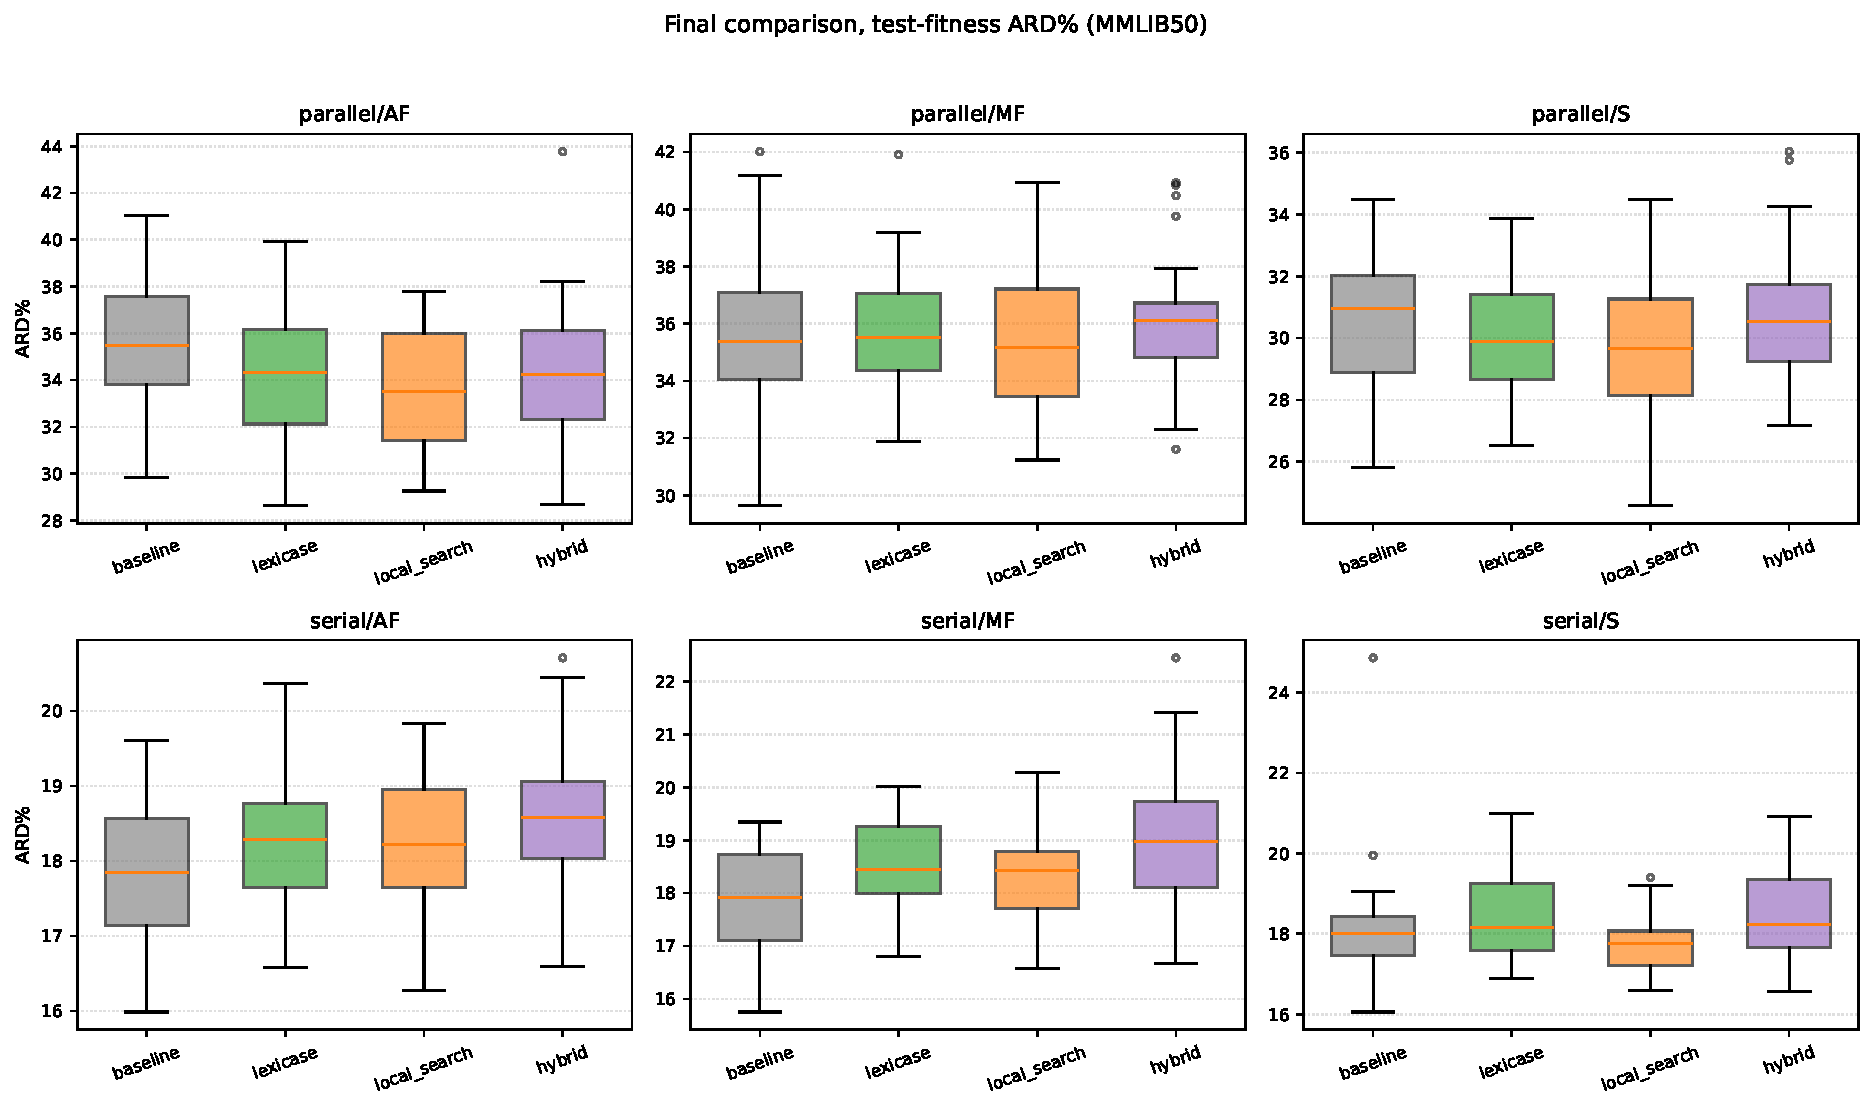
\includegraphics[width=0.95\textwidth]{img/generated/final_comparison_boxplot_mmlib50.pdf}
  \caption{Final comparison boxplot, all four jointly ranked conditions,
  MMLIB50, one panel per (SGS, strategy) cell.}
  \label{fig:final-comparison-boxplot}
\end{figure}

\begin{figure}[htbp]
  \centering
  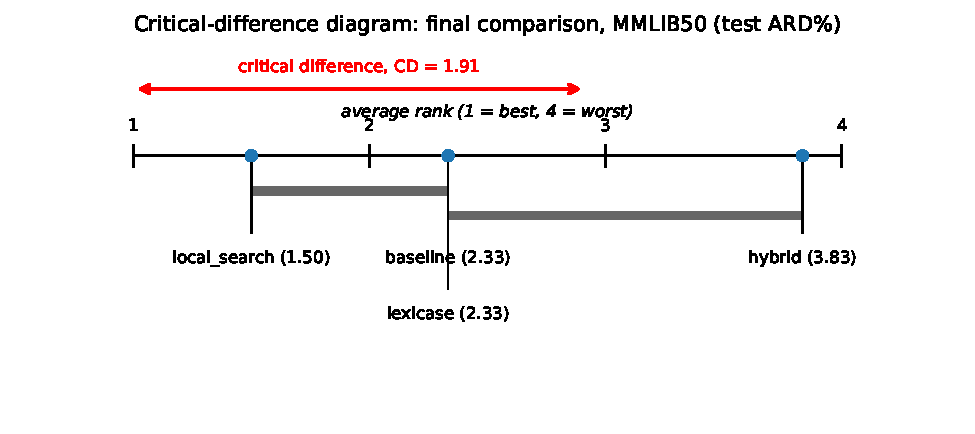
\includegraphics[width=0.85\textwidth]{img/generated/final_comparison_cd_mmlib50.pdf}
  \caption[Critical-difference diagram, final comparison, MMLIB50]{Critical-difference
  diagram, final comparison, MMLIB50 (test ARD\%). The Friedman test is
  significant ($p=0.0169$), so this diagram is meaningful: local search
  separates from hybrid by more than the critical difference (CD $=1.91$),
  while baseline and lexicase, tied at average rank 2.33, sit between them
  and are not statistically distinguishable from either.}
  \label{fig:final-comparison-cd}
\end{figure}

Figure~\ref{fig:final-comparison-cd} packs several pieces of information
into one plot, so it is worth reading it element by element. The
horizontal axis is average rank across the six (SGS, strategy) cells,
running from 1 (best, i.e.\ lowest mean ARD\%) to 4 (worst); each
condition's dot marks its own average rank from
Table~\ref{tab:method-rankings} (local search 1.50, baseline and lexicase
tied at 2.33, hybrid 3.83). The red double-headed arrow at the top is not a
comparison between two specific conditions: it is a ruler, showing how long
one critical difference (CD $=1.91$ rank units, computed from the Nemenyi
formula for $k=4$ conditions and $N=6$ blocks/cells) is on this axis, so
the reader can visually judge distances between dots against it. The thick
grey bars beneath the axis are the actual pairwise verdicts: a bar spanning
two or more dots means those conditions' average ranks are \emph{closer
together than one CD}, i.e.\ not distinguishable from chance at this
sample size; conditions with \emph{no} bar connecting them (here, local
search and hybrid, $3.83-1.50=2.33 > \mathrm{CD}$) are the pairs the
diagram identifies as genuinely different. Reading the two bars together:
local search's rank is close enough to baseline/lexicase's to share a bar
with them, and baseline/lexicase's rank is in turn close enough to
hybrid's to share a second, separate bar with it, but local search and
hybrid themselves, at the two ends, are far enough apart that no single bar
spans both, which is exactly what \changedC{``local search significantly
outranks hybrid, with baseline and lexicase in between and not clearly
separable from either neighbour''} looks like in this convention.

\begin{table}[htbp]
  \centering
  \small
  \caption[Method rankings, MMLIB100]{Average rank (1 = best, 4 = worst)
  across the six (SGS, strategy) cells, MMLIB100, test and train fitness.
  Neither Friedman test is significant (test: $\chi^2 = 1.40$, $p = 0.706$;
  train: $\chi^2 = 4.20$, $p = 0.241$; 6 blocks, 4 conditions).}
  \label{tab:method-rankings-mmlib100}
  \begin{tabular}{lrr}
    \toprule
    \textbf{Condition} & \textbf{Avg.\ rank (test)} & \textbf{Avg.\ rank (train)} \\
    \midrule
    Baseline     & 2.00 & 2.50 \\
    Lexicase     & 2.50 & 1.67 \\
    Hybrid       & 2.67 & 2.67 \\
    Local search & 2.83 & 3.17 \\
    \bottomrule
  \end{tabular}
\end{table}

\begin{figure}[htbp]
  \centering
  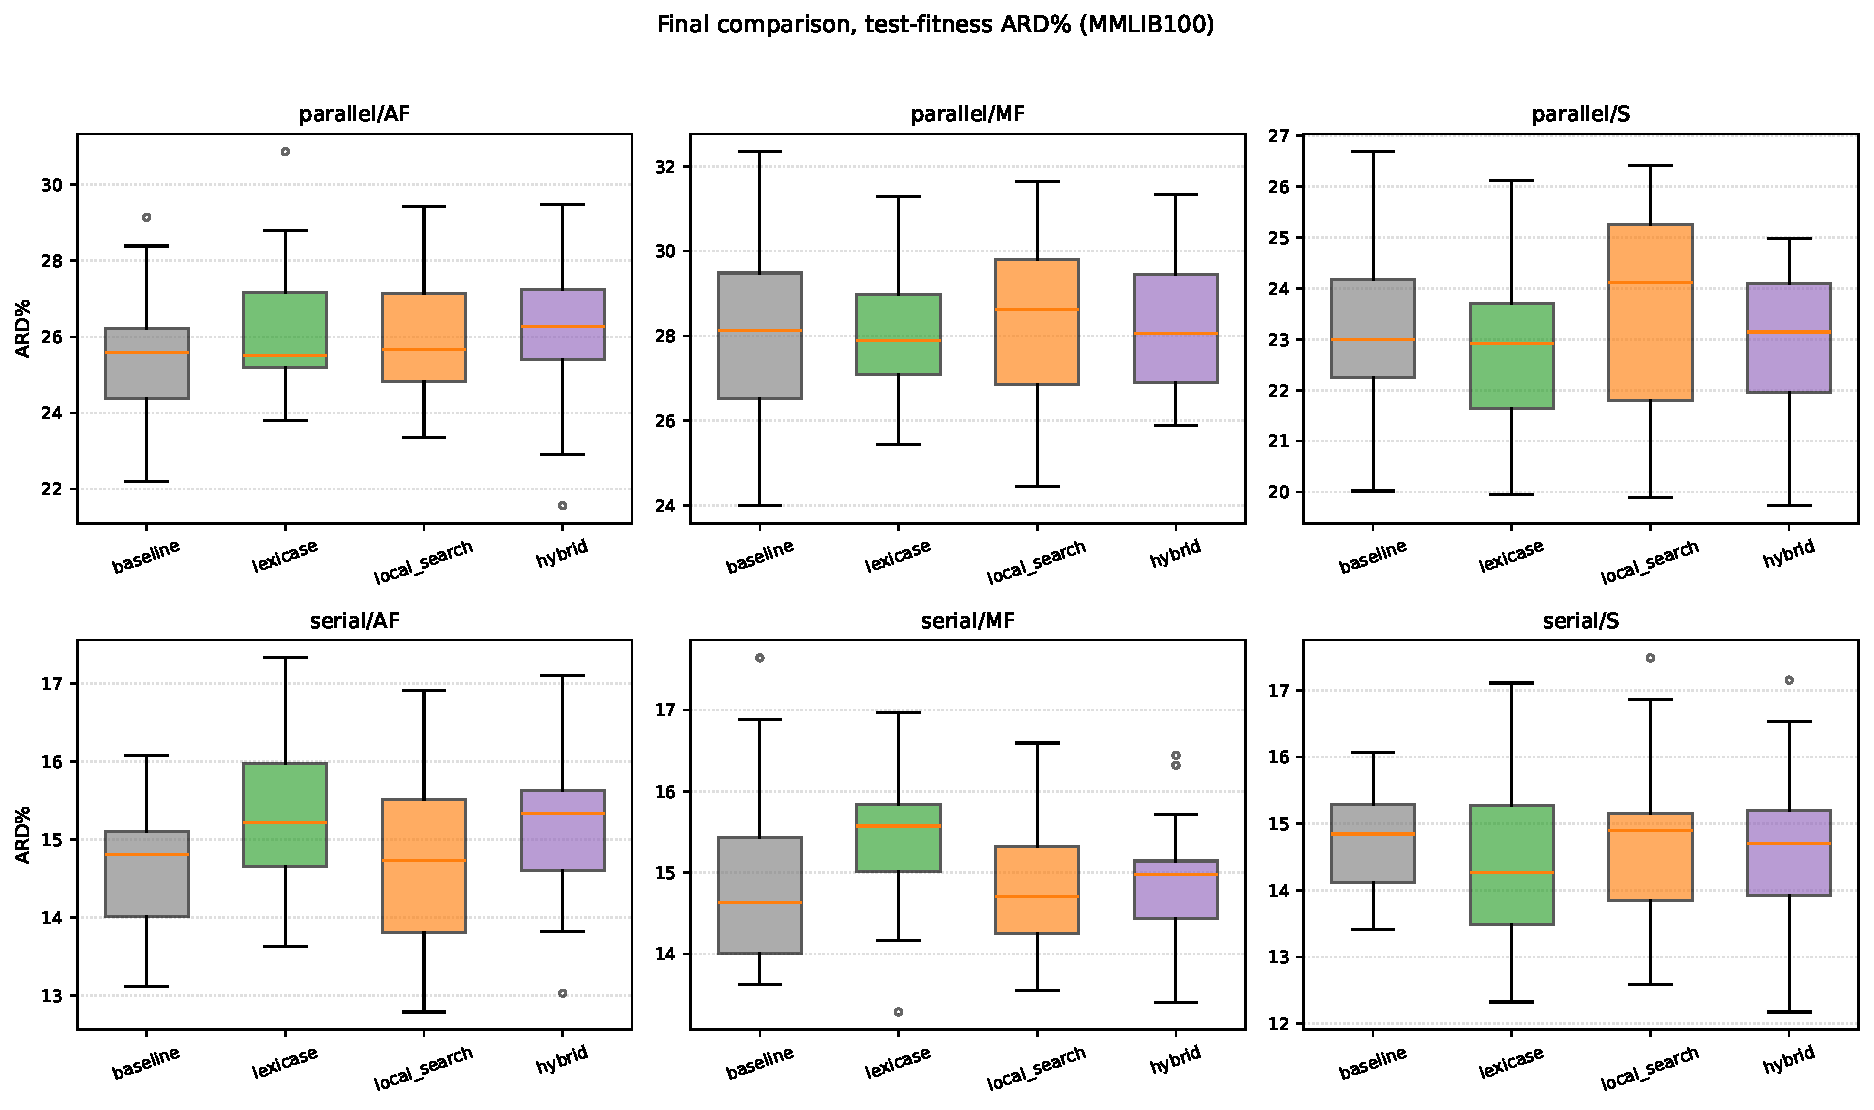
\includegraphics[width=0.95\textwidth]{img/generated/final_comparison_boxplot_mmlib100.pdf}
  \caption{Final comparison boxplot, all four jointly ranked conditions,
  MMLIB100, one panel per (SGS, strategy) cell, same layout as
  Figure~\ref{fig:final-comparison-boxplot}. Note local search's spread
  overlapping baseline's in every panel, consistent with
  Table~\ref{tab:method-rankings-mmlib100}'s non-significant Friedman test.}
  \label{fig:final-comparison-boxplot-mmlib100}
\end{figure}

A critical-difference diagram is deliberately \emph{not} presented for
MMLIB100's ranking, consistent with the convention fixed in
Section~\ref{subsec:statistical-methodology}: a CD diagram is only drawn
where the underlying Friedman test is itself significant, and neither
MMLIB100 Friedman test clears that bar (Table~\ref{tab:method-rankings-mmlib100}).

The joint ranking adds a finding that none of the three pairwise
subsections could show on its own: the Friedman test across the six cells
is significant ($p=0.0169$), so the difference between local search's
average rank (1.50) and hybrid's (3.83) is not attributable to chance, even
though neither individual pairwise comparison against baseline reached
significance in every cell. Two observations stand out. First, local
search alone achieves the best average test-fitness rank of the four, a
more favourable summary than Section~\ref{subsec:localsearch-eval}'s
cell-by-cell significance table might suggest on its own, precisely because
ranking rewards a method that is consistently a little better even where
no single cell clears the $p<0.05$ bar. Second, and more strikingly,
\emph{hybrid}, lexicase and local search combined, ranks worst of the four,
not best: Table~\ref{tab:lexicase-significance}-style pairwise tests (not
reproduced in full here for space) show hybrid significantly worse than
baseline on test fitness in three of six cells (all three under serial
SGS), against a single significant win under parallel/activity-first.
Combining the two individually defensible mechanisms does not add their
benefits; if anything, it compounds whatever is producing lexicase's
serial-SGS generalisation gap (Section~\ref{subsec:lexicase-eval}), since
hybrid inherits lexicase's selection mechanism on top of local search's own
refinement step. \changed{A plausible-looking combination of two components
that each showed some individual promise thus underperforms both
components individually, and is not recommended by this evidence as the
thesis's final proposed configuration.}

\textbf{Scalability validation.} This is the second, and more consequential,
instance in this chapter of an MMLIB50 finding not surviving the move to
MMLIB100. Table~\ref{tab:method-rankings-mmlib100} shows local search
falling from the \emph{best} average test-fitness rank on MMLIB50 (1.50) to
the \emph{worst} on MMLIB100 (2.83), with baseline itself now ranking best
(2.00); neither MMLIB100 Friedman test reaches significance, so, unlike
MMLIB50, the ranking differences at this scale are not distinguishable from
chance in the first place. Lexicase's relative position is more stable, it
ranks second-worst on MMLIB100 test fitness (2.50, tied with its own
MMLIB50 rank) while actually improving to the best rank on MMLIB100
\emph{training} fitness (1.67), consistent with
Section~\ref{subsec:lexicase-eval}'s finding that its training advantage is
real and, if anything, strengthens with scale even as its test advantage
does not. The practical implication is that this chapter's MMLIB50-only
final ranking, in particular its endorsement of local search as the
best-performing single condition, should not be read as a scale-independent
verdict: at MMLIB100, no condition in this four-way comparison
distinguishes itself from baseline with statistical confidence, and the
one candidate that appeared to (local search) \changed{owed its favourable
average rank to a consistent but individually non-significant advantage
across cells, an advantage that inverts once the same protocol is applied
to larger instances.}
Of the three comprehensive-stage candidates, this leaves NR terminals
(Section~\ref{subsec:nr-eval}), evaluated separately from this ranking for
the instance-set reasons already stated, as the only one whose evidence for
a real effect strengthens rather than weakens under scaling.

\textbf{Breakdown by instance characteristics.}
\changed{Because every test class corresponds to one OS/RF/RS combination
(Section~\ref{subsec:instance-sampling}), the per-class results show
directly how the conditions behave across instance characteristics.
Table~\ref{tab:per-class-breakdown} reports, for each of the ten MMLIB50
test instances, its indicators (computed directly from the instance; RS is
the mean over the two renewable resources) and the mean held-out deviation
of the four jointly ranked conditions (serial SGS, activity-first, 30
seeds, feasible runs). Two observations stand out. First, difficulty is
driven far more by the instance characteristics than by the choice of
condition: the tightly resource-constrained, high-RF classes
(\texttt{J5011}: OS 0.25, RF 1.00, RS 0.25; \texttt{J501};
\texttt{J5081}) dominate the aggregate ARD\%, while every condition
solves the loosely constrained classes ($\mathrm{RS} \ge 0.75$) at or
near the CPM bound. Second, the differences between conditions within a
class are small relative to the differences across classes, consistent
with the non-significant aggregate ranking at this scale; no condition is
systematically better on any particular OS/RF/RS regime.}

\begin{table}[htbp]
  \centering
  \small
  \shrinktofit{%
  \caption[Per-class breakdown of the final comparison]{\changed{Mean
  held-out deviation (\%) per test class, MMLIB50, serial SGS,
  activity-first, with each class's OS/RF/RS indicators computed from the
  instance. Rows are the ten stratified test instances (one per class).}}
  \label{tab:per-class-breakdown}
  \begin{tabular}{lrrrrrrr}
    \toprule
    \textbf{Instance} & \textbf{OS} & \textbf{RF} & \textbf{RS} & \textbf{Baseline} & \textbf{Lexicase} & \textbf{Local search} & \textbf{Hybrid} \\
    \midrule
    \texttt{J501\_5}  & 0.25 & 0.50 & 0.36 &  33.61 &  36.11 &  36.11 &  36.94 \\
    \texttt{J5011\_5} & 0.25 & 1.00 & 0.25 & 102.71 & 101.67 & 102.50 & 102.92 \\
    \texttt{J5021\_5} & 0.25 & 1.00 & 0.50 &   8.33 &   8.33 &   8.12 &   8.12 \\
    \texttt{J5031\_5} & 0.25 & 1.00 & 0.75 &   0.00 &   0.00 &   0.00 &   0.00 \\
    \texttt{J5041\_5} & 0.50 & 0.50 & 0.44 &   4.24 &   4.44 &   3.94 &   4.75 \\
    \texttt{J5051\_5} & 0.50 & 0.50 & 0.90 &   0.00 &   0.00 &   0.00 &   0.00 \\
    \texttt{J5061\_5} & 0.50 & 0.50 & 1.27 &   0.24 &   0.24 &   0.60 &   0.71 \\
    \texttt{J5071\_5} & 0.50 & 1.00 & 0.75 &   0.00 &   0.00 &   0.00 &   0.37 \\
    \texttt{J5081\_5} & 0.75 & 1.00 & 0.25 &  26.67 &  28.53 &  27.98 &  27.60 \\
    \texttt{J5091\_5} & 0.75 & 1.00 & 0.50 &   2.29 &   4.00 &   3.14 &   4.19 \\
    \bottomrule
  \end{tabular}%
  }
\end{table}

\subsection{Re-evaluation on the full 108-class test set}
\label{subsec:full108}

\changedB{Every test figure reported so far rests on a deliberately small
held-out set. To keep the comprehensive stage within the available compute
budget, each cell was trained and tested on a stratified subset of ten
classes out of each benchmark's 108 (Section~\ref{subsec:instance-sampling}),
and because that reduction applies to the test split as well, every mean test
ARD\% above is an average over just ten instances, one per sampled class. A
reasonable worry is that ten instances are too few to characterise a rule's
true test behaviour, and that some of the conclusions drawn above are
sensitive to which ten classes were sampled. This section addresses that
worry directly by re-evaluating the evolved rules on the complete 108-class
test set.}

\changedB{The procedure is cheap and changes nothing about how
the rules were produced. For every one of the 2160 cells (six conditions,
six SGS/strategy combinations, two benchmarks, thirty seeds) we take the
rule that cell already deployed, the validation-selected best individual that
produced its reported test figure, and re-evaluate it, with no further
evolution, on case 5 of every class from 1 to 108. This gives 108 held-out
test instances per benchmark in place of the original ten. The re-evaluation
reuses each condition's own conventions unchanged: the NR-preserving
instances and the NR terminal set for \texttt{nr} and \texttt{baseline\_nr},
the paper's renewable-only conversion for the other four conditions, and the
cell's own SGS and decision strategy. The metrics are unchanged as well:
ARD\%, the makespan's percentage deviation from the critical-path lower
bound averaged over the instances a rule schedules feasibly, and the
feasibility rate, the fraction of the 108 instances scheduled feasibly. No
population and no generations are involved, only one schedule construction
per instance, so the whole 2160-cell re-evaluation runs on a single
workstation without special resources.}

\begin{table}[htbp]
  \centering
  \small
  \caption[Full 108-class re-evaluation, renewable conditions]{\changedB{Test
  ARD\% on the full 108-class held-out set for the four conditions that share
  the renewable-only instance set. Baseline's ten-class figure is repeated
  from the tables above as the reference point for the shift; the other three
  conditions' ten-class figures lie within $1.2$ percentage points of
  baseline's in every cell and are omitted. All four conditions are
  $100\%$ feasible on both the ten-class and the 108-class test set.}}
  \label{tab:full108-renewable}
  \begin{tabular}{lrrrrr}
    \toprule
    & \multicolumn{2}{c}{\textbf{baseline}} & \textbf{lexicase}
    & \textbf{loc.\ search} & \textbf{hybrid} \\
    \cmidrule(lr){2-3}\cmidrule(lr){4-4}\cmidrule(lr){5-5}\cmidrule(lr){6-6}
    \textbf{SGS/strat.} & \textbf{10 cls} & \textbf{108 cls}
    & \textbf{108 cls} & \textbf{108 cls} & \textbf{108 cls} \\
    \midrule
    \multicolumn{6}{l}{\textit{MMLIB50}} \\
    Serial/AF   & 18.3 & 13.1 & 13.2 & 13.1 & 13.2 \\
    Serial/MF   & 18.1 & 13.1 & 13.0 & 13.1 & 13.1 \\
    Serial/S    & 18.3 & 13.1 & 13.3 & 13.3 & 13.5 \\
    Parallel/AF & 34.7 & 23.5 & 24.0 & 23.0 & 24.1 \\
    Parallel/MF & 36.0 & 24.7 & 24.8 & 24.9 & 24.7 \\
    Parallel/S  & 31.6 & 21.1 & 21.2 & 20.6 & 21.1 \\
    \midrule
    \multicolumn{6}{l}{\textit{MMLIB100}} \\
    Serial/AF   & 14.4 & 11.7 & 11.7 & 11.8 & 11.5 \\
    Serial/MF   & 14.6 & 11.9 & 11.8 & 11.9 & 11.6 \\
    Serial/S    & 14.6 & 11.8 & 11.9 & 11.9 & 11.9 \\
    Parallel/AF & 25.5 & 19.8 & 19.7 & 19.8 & 19.6 \\
    Parallel/MF & 28.0 & 21.3 & 21.1 & 21.3 & 21.1 \\
    Parallel/S  & 23.2 & 17.3 & 17.0 & 17.2 & 17.1 \\
    \bottomrule
  \end{tabular}
\end{table}

\changedB{Table~\ref{tab:full108-renewable} gives the outcome for the four
conditions on the renewable-only instances, and two facts hold across all
twelve cells. First, enlarging the test set from ten classes to 108 lowers
ARD\% everywhere, by $6.2$ percentage points on average and by between $2.1$
and $11.4$ points depending on the cell. \changedC{The shift is chiefly a
\changedD{sampling} effect: easy and hard instances are not represented in the ten
stratified classes in their true benchmark proportions, and the ten happen
to over-sample the tightly constrained, high-ARD\% end of the OS/RF/RS
grid (visible directly in Table~\ref{tab:per-class-breakdown}), whereas
the 108-class set contains every class and so restores the benchmark's
actual mix of easy and hard instances.} The ten-class test set was thus a
small and, as it turns out, somewhat pessimistic sample, so the absolute test
figures reported earlier are, if anything, conservative rather than
flattering. Second, and more important for the argument of this chapter, the
four conditions stay indistinguishable at full test scale exactly as they
were at ten classes: on 108 classes lexicase, local search, and hybrid each
remain within $0.65$ percentage points of baseline in every cell. The
near-null result for these three modifications on the renewable instances is
therefore not an artefact of the reduced test set; it survives evaluation on
the complete held-out distribution.}

\begin{table}[htbp]
  \centering
  \small
  \caption[Full 108-class re-evaluation, NR conditions]{\changedB{The NR pair
  on their NR-preserving instances. ARD\% is on the full 108-class test set;
  feasibility is shown for both the ten-class (\emph{feas.\ 10}) and the
  108-class (\emph{feas.\ 108}) sets so the change of scale is visible. Lower
  ARD\% and higher feasibility are better.}}
  \label{tab:full108-nr}
  \begin{tabular}{lrrrrrr}
    \toprule
    & \multicolumn{3}{c}{\textbf{\texttt{baseline\_nr}}}
    & \multicolumn{3}{c}{\textbf{NR terminals}} \\
    \cmidrule(lr){2-4}\cmidrule(lr){5-7}
    \textbf{SGS/strat.} & \textbf{ARD\%} & \textbf{feas.\,10}
    & \textbf{feas.\,108} & \textbf{ARD\%} & \textbf{feas.\,10}
    & \textbf{feas.\,108} \\
    \midrule
    \multicolumn{7}{l}{\textit{MMLIB50}} \\
    Serial/AF   & 126.4 & 70\% & 84\% & 88.4  & 84\% & 70\% \\
    Serial/MF   & 125.7 & 68\% & 84\% & 94.5  & 83\% & 75\% \\
    Serial/S    & 132.0 & 70\% & 89\% & 94.1  & 85\% & 85\% \\
    Parallel/AF & 115.8 & 67\% & 80\% & 107.2 & 85\% & 79\% \\
    Parallel/MF & 117.9 & 68\% & 83\% & 105.7 & 82\% & 79\% \\
    Parallel/S  & 120.0 & 67\% & 82\% & 113.6 & 83\% & 90\% \\
    \midrule
    \multicolumn{7}{l}{\textit{MMLIB100}} \\
    Serial/AF   & 116.1 & 85\% & 86\% & 87.6  & 98\% & 84\% \\
    Serial/MF   & 116.1 & 88\% & 88\% & 90.2  & 98\% & 87\% \\
    Serial/S    & 122.9 & 91\% & 89\% & 97.9  & 99\% & 96\% \\
    Parallel/AF & 111.1 & 78\% & 83\% & 93.8  & 89\% & 85\% \\
    Parallel/MF & 110.1 & 81\% & 85\% & 93.7  & 88\% & 82\% \\
    Parallel/S  & 118.7 & 81\% & 88\% & 97.8  & 87\% & 87\% \\
    \bottomrule
  \end{tabular}
\end{table}

\changedB{Table~\ref{tab:full108-nr} tells a more nuanced story for the NR
pair. The schedule-quality advantage of NR terminals is untouched by the
change of scale: their 108-class ARD\% is below \texttt{baseline\_nr}'s in
all twelve cells, by margins from about $6$ to nearly $40$ percentage points,
in line with the ten-class result of Section~\ref{subsec:nr-eval}. What does
not carry over cleanly is the feasibility advantage. On the ten-class test
set NR terminals scheduled a larger fraction of instances feasibly than
\texttt{baseline\_nr} in every one of the twelve cells; on the full 108-class
set this gap closes to near-parity on MMLIB100 and reverses on MMLIB50, where
NR terminals' feasibility sits at or below \texttt{baseline\_nr}'s in five of
the six cells. The reading consistent with both metrics is that NR terminals
produce markedly better schedules on the instances they solve, but that part
of their feasibility gain on the ten sampled classes is an in-distribution
effect: the rule, evolved on three cases of those same ten classes, extends
its quality advantage to the 98 unseen classes far more reliably than it
extends its feasibility advantage. This qualifies, without overturning, the
feasibility claim of Section~\ref{subsec:nr-eval}; the central and larger
schedule-quality result is unaffected.}

\changedB{The feasibility reversal appears only at the larger test scale
because the ten sampled classes are the very classes each rule was trained
on, so the ten-class figure measures in-distribution feasibility, while the
98 classes added to reach 108 are unseen. Splitting the 108-class feasibility
into these two parts (Table~\ref{tab:full108-nr-generalisation}) isolates the
effect. On the ten seen classes NR terminals are far more feasible than
\texttt{baseline\_nr} ($84\%$ against $68\%$ on MMLIB50, $93\%$ against
$84\%$ on MMLIB100), which is the gain reported in
Section~\ref{subsec:nr-eval}. On the 98 unseen classes that gain disappears:
NR terminals fall to $79\%$ and $86\%$ while \texttt{baseline\_nr} rises to
$85\%$ and $87\%$, so the two are level or NR terminals sit marginally
behind. The asymmetry is mechanistic. \texttt{baseline\_nr} cannot see the
non-renewable state, so it has no class-specific budget management to overfit
and its feasibility simply tracks class difficulty, and because the sampled
ten classes are harder than the benchmark average (the same reason ARD\%
falls when the test set is enlarged) its feasibility rises on the broader
set. NR terminals give the rule exactly the expressiveness needed to secure
feasibility on the classes it trains on, and that part of the benefit does
not carry to unseen classes. Schedule quality transfers because a good
relative priority ordering generalises across classes; the absolute
non-renewable budget thresholds that decide feasibility do not.}

\begin{table}[htbp]
  \centering
  \small
  \caption[Feasibility on seen versus unseen classes]{\changedB{Feasibility
  rate of the NR pair split into the ten training-adjacent (seen) classes and
  the 98 unseen classes that make up the rest of the 108-class test set.
  The \emph{all 108} column is the feasibility of
  Table~\ref{tab:full108-nr}. NR terminals' feasibility advantage is confined
  to the seen classes.}}
  \label{tab:full108-nr-generalisation}
  \begin{tabular}{llrrr}
    \toprule
    \textbf{Benchmark} & \textbf{Condition} & \textbf{seen (10)}
    & \textbf{unseen (98)} & \textbf{all 108} \\
    \midrule
    \multirow{2}{*}{MMLIB50}
      & \texttt{baseline\_nr} & 68\% & 85\% & 84\% \\
      & NR terminals          & 84\% & 79\% & 80\% \\
    \addlinespace
    \multirow{2}{*}{MMLIB100}
      & \texttt{baseline\_nr} & 84\% & 87\% & 86\% \\
      & NR terminals          & 93\% & 86\% & 87\% \\
    \bottomrule
  \end{tabular}
\end{table}

\changedC{\textbf{Breakdown by instance characteristics.} With 108 test
instances per benchmark, the re-evaluation is also large enough to be
split by instance characteristics, which the ten-class test set was not.
Because every class realises one OS/RF/RS combination and the indicators
are computed directly from each instance (as in
Table~\ref{tab:per-class-breakdown}),
Tables~\ref{tab:full108-os}--\ref{tab:full108-rs} report the same
108-class test results separately for every value of each indicator: each
entry is the mean test ARD\% computed only over the instances with the
given OS, RF, or RS value, pooled across all six (SGS, strategy) cells
and 30 seeds. OS and RF take exactly three and two values on the MMLIB
grid; RS is continuous, so it is grouped into tight
($\mathrm{RS} \le 0.5$), medium ($0.5 < \mathrm{RS} \le 1$) and
effectively unconstrained ($\mathrm{RS} > 1$) instances. The four
renewable-instance conditions are $100\%$ feasible everywhere, so only
ARD\% is shown for them; for the NR pair, which runs on the NR-preserving
instances and is not comparable in magnitude to the other four, the
feasibility rate over the group is given in parentheses.}

\begin{table}[htbp]
  \centering
  \small
  \caption[108-class breakdown by order strength]{\changedC{Test ARD\%
  on the full 108-class set, computed only over instances with the given
  order strength (OS), pooled over all six (SGS, strategy) cells and 30
  seeds. NR-pair entries (their own NR-preserving instance set) carry the
  group's feasibility rate in parentheses; the four renewable conditions
  are $100\%$ feasible throughout.}}
  \label{tab:full108-os}
  \begin{tabular}{lrrr}
    \toprule
    \textbf{Condition} & $\mathrm{OS} = 0.25$ & $\mathrm{OS} = 0.50$ & $\mathrm{OS} = 0.75$ \\
    \midrule
    \multicolumn{4}{l}{\textit{MMLIB50}} \\
    Baseline & 23.6 & 18.3 & 12.3 \\
    Lexicase & 23.8 & 18.4 & 12.6 \\
    Local search & 23.6 & 18.2 & 12.2 \\
    Hybrid & 24.0 & 18.3 & 12.5 \\
    \texttt{baseline\_nr} & 122.0 (85\%) & 125.5 (84\%) & 126.6 (82\%) \\
    NR terminals & 106.9 (83\%) & 103.0 (81\%) & 97.5 (75\%) \\
    \midrule
    \multicolumn{4}{l}{\textit{MMLIB100}} \\
    Baseline & 14.8 & 19.1 & 13.0 \\
    Lexicase & 14.5 & 18.8 & 13.2 \\
    Local search & 14.8 & 19.1 & 13.1 \\
    Hybrid & 14.5 & 18.9 & 13.0 \\
    \texttt{baseline\_nr} & 115.0 (88\%) & 126.9 (88\%) & 109.4 (83\%) \\
    NR terminals & 95.9 (95\%) & 99.9 (87\%) & 86.1 (79\%) \\
    \bottomrule
  \end{tabular}
\end{table}

\begin{table}[htbp]
  \centering
  \small
  \caption[108-class breakdown by resource factor]{\changedC{Test ARD\%
  on the full 108-class set, computed only over instances with the given
  resource factor (RF); layout as in Table~\ref{tab:full108-os}.}}
  \label{tab:full108-rf}
  \begin{tabular}{lrr}
    \toprule
    \textbf{Condition} & $\mathrm{RF} = 0.50$ & $\mathrm{RF} = 1.00$ \\
    \midrule
    \multicolumn{3}{l}{\textit{MMLIB50}} \\
    Baseline & 8.2 & 28.0 \\
    Lexicase & 8.3 & 28.2 \\
    Local search & 8.2 & 27.8 \\
    Hybrid & 8.3 & 28.3 \\
    \texttt{baseline\_nr} & 104.8 (83\%) & 144.0 (85\%) \\
    NR terminals & 83.9 (77\%) & 120.0 (83\%) \\
    \midrule
    \multicolumn{3}{l}{\textit{MMLIB100}} \\
    Baseline & 6.1 & 25.1 \\
    Lexicase & 6.0 & 25.0 \\
    Local search & 6.2 & 25.1 \\
    Hybrid & 5.9 & 25.1 \\
    \texttt{baseline\_nr} & 95.4 (83\%) & 137.4 (90\%) \\
    NR terminals & 76.7 (85\%) & 110.9 (89\%) \\
    \bottomrule
  \end{tabular}
\end{table}

\begin{table}[htbp]
  \centering
  \small
  \caption[108-class breakdown by resource strength]{\changedC{Test ARD\%
  on the full 108-class set, computed only over instances in the given
  resource-strength (RS) range; layout as in
  Table~\ref{tab:full108-os}.}}
  \label{tab:full108-rs}
  \begin{tabular}{lrrr}
    \toprule
    \textbf{Condition} & $\mathrm{RS} \le 0.5$ & $0.5 < \mathrm{RS} \le 1$ & $\mathrm{RS} > 1$ \\
    \midrule
    \multicolumn{4}{l}{\textit{MMLIB50}} \\
    Baseline & 43.7 & 4.6 & 0.5 \\
    Lexicase & 43.9 & 4.8 & 0.4 \\
    Local search & 43.6 & 4.5 & 0.4 \\
    Hybrid & 44.1 & 4.7 & 0.4 \\
    \texttt{baseline\_nr} & 157.9 (78\%) & 109.5 (87\%) & 103.0 (90\%) \\
    NR terminals & 135.0 (75\%) & 87.8 (81\%) & 80.2 (86\%) \\
    \midrule
    \multicolumn{4}{l}{\textit{MMLIB100}} \\
    Baseline & 31.2 & 2.8 & 0.5 \\
    Lexicase & 30.9 & 2.9 & 0.5 \\
    Local search & 31.3 & 2.8 & 0.5 \\
    Hybrid & 31.1 & 2.7 & 0.3 \\
    \texttt{baseline\_nr} & 140.5 (83\%) & 99.3 (90\%) & 97.1 (87\%) \\
    NR terminals & 113.8 (81\%) & 80.4 (91\%) & 77.2 (96\%) \\
    \bottomrule
  \end{tabular}
\end{table}

\changedC{Three observations follow. First, difficulty is driven
overwhelmingly by the resource indicators, not by the network shape:
moving from $\mathrm{RF} = 0.50$ to $\mathrm{RF} = 1.00$ roughly triples
the renewable conditions' ARD\% (8.2 to 28.0 on MMLIB50), and moving
from tight to effectively unconstrained RS spans almost the entire
observed range (43.7 down to 0.5), while OS produces the smallest and
least systematic differences (on MMLIB100 the middle level
$\mathrm{OS} = 0.50$ is the hardest). Second, the four renewable
conditions remain indistinguishable \emph{within every single indicator
level}: the largest spread between them in any cell of the three tables
is $0.5$ percentage points, so the earlier per-class observation that no
condition is systematically better on any particular OS/RF/RS regime
(Table~\ref{tab:per-class-breakdown}) holds on the complete test
distribution, not just the ten stratified classes. Third, NR terminals'
schedule-quality advantage over \texttt{baseline\_nr} is present at
every value of every indicator on both benchmarks (by 15--29 points on
MMLIB50 and 19--27 points on MMLIB100), while their MMLIB50 feasibility
shortfall is spread fairly evenly across the levels rather than
concentrated in one regime, consistent with
Table~\ref{tab:full108-nr-generalisation}'s reading that the shortfall
follows class identity (seen versus unseen), not any particular
instance characteristic.}

\changedD{The feasibility rates of Table~\ref{tab:full108-rs} show one
further pattern: as RS grows and the renewable constraints loosen, the
NR-aware rules schedule an increasing share of instances feasibly, on
MMLIB100 rising from $81\%$ on the tight instances to $96\%$ on the
effectively unconstrained ones, while \texttt{baseline\_nr} shows no such
progression there ($83$--$90\%$, with no gain at $\mathrm{RS} > 1$). This
is what the terminals' mechanism predicts: the looser the renewable
constraints, the more feasibility is decided by the non-renewable budget
alone, which is precisely the state the NR terminals expose and the
baseline cannot see. On MMLIB50 both conditions' feasibility improves with
RS at a similar rate, so the separation is clearly visible only at the
larger instance size.}

Taken together, Sections~\ref{sec:parameter-sensitivity}
through~\ref{sec:benchmark-comparison} tell a coherent
story. Of a wide field of candidate ideas, screened
cheaply and then narrowed to three, only NR terminals produced a result
that is large, consistent, and free of the SGS-dependent reversals that
qualify the other two; lexicase selection and critical-path local search
each show a genuine, mechanistically interpretable signal, but a signal
that is smaller, direction-dependent, and, in lexicase's case, prone to not
generalising past the training set; and the naive combination of the two
weaker methods performs worse than either alone. Chapter~\ref{chap:conclusion}
takes up the question of what this pattern of results implies for the
thesis's research questions and for GPHH-based scheduling research more
broadly.

\section{Complexity analysis and limitations}
\label{sec:complexity-limitations}

The cost of a single GP run is dominated by fitness evaluation: each of the
$N_{\text{pop}}$ individuals must decode a schedule via the SGS on every
training instance, once per generation, so a single run's cost scales as
$O(N_{\text{pop}} \times N_{\text{gen}} \times N_{\text{inst}} \times
C_{\text{decode}})$, where $C_{\text{decode}}$ itself grows with the
number of activities and modes per instance. This is why MMLIB100 costs
substantially more per run
than MMLIB50 at the same population and generation budget, purely from
doubling the activity count, and why \changed{the training times reported
by Tian et al.~\cite{Tian2024GPHH}} range from a few
hundred seconds for parallel SGS on MMLIB50 up to tens of thousands of
seconds for serial SGS on the largest MMLIB+ instances at the full
pop=1\,000/gen=50 budget. \changed{This cost structure is why the
comprehensive stage evaluates every condition on a
stratified $n_{\text{classes}}=10$ subsample of each dataset's full 108
classes rather than on all of them
(Section~\ref{subsec:instance-sampling}): all planned runs on that
subsample were completed, but reproducing the paper's
own full-class evaluation for the baseline alone, let alone six conditions
across two SGS types and three decision strategies, \changedC{would have
taken several hundred days of computation, more than could be completed
within the time frame of this thesis (MetaCentrum itself imposes no such
limit; the constraint was the thesis's schedule)}.}

\changed{The realised cost of the comprehensive stage can be stated
exactly, since every result file records its own wall-clock running time.
The 2\,160 comprehensive-stage runs (1\,080 per benchmark) took a combined
$17\,187$ hours of wall-clock time, about $716$ days, corresponding to
roughly $5\,700$ CPU-days at the 8 cores allocated per run. A single
MMLIB50 run took $3.4$ hours on average (median $2.3$, range
$0.7$--$25.1$); a single MMLIB100 run took $12.5$ hours on average (median
$10.2$, range $2.8$--$55.9$), confirming the cost increase from doubling
the instance size. By condition, \texttt{local\_search} and \texttt{hybrid}
were indeed the most expensive, averaging $4.5$--$4.6$ hours per MMLIB50
run and $15.7$--$16.3$ hours per MMLIB100 run against the baseline's
$2.8$ and $10.0$ hours; by decoding scheme, serial-SGS runs took roughly
twice as long as parallel ones on average ($5.0$ versus $1.8$ hours on
MMLIB50, $16.7$ versus $8.4$ hours on MMLIB100). Including the
exploratory stage, preliminary and repeated jobs, and all side
experiments, the MetaCentrum account used for this thesis executed
$30\,287$ jobs consuming roughly $11\,600$ CPU-days in total. These times
were measured on heterogeneous, scheduler-assigned grid nodes
(Table~\ref{tab:hw-sw-config}) and are therefore indicative rather than
exactly comparable across runs.}

The three proposed extensions add comparatively little to this base cost,
but not equally so. NR terminals are the cheapest: each of the three added
terminals is a constant-time lookup against a per-instance cache computed
once before the run begins, so the per-individual evaluation cost is
essentially unchanged from the baseline. Epsilon-lexicase selection is
more expensive per selection event than tournament selection, since it may
filter over as many training cases as it takes to narrow the candidate
pool to one survivor, rather than comparing a fixed, small tournament
sample, though this cost is still minor relative to fitness evaluation
itself. Critical-path local search is the most expensive of the three: its
hill-climb runs for up to ten iterations on the top 8\% of the population,
every generation, and each iteration re-decodes the candidate schedule to
check feasibility, which \changed{made \texttt{local\_search} and
\texttt{hybrid} the most expensive conditions in the walltime estimates
used for PBS job scheduling. One combination of the full
paper-scale grid, the \texttt{hybrid} condition under serial SGS with the
mode-first strategy on the largest MMLIB+ instances, was excluded from the
matrix entirely on this basis: \changedC{even a single seed's estimated
running time was so long that the full 30-seed cell could not have
finished before this thesis was due}.}

Two further limitations accompany the cost
model. First, every comprehensive-stage run in this chapter used
population 1\,000 and 50 generations, matching the paper's own
configuration; whether the qualitative pattern of results, in particular
lexicase's SGS-dependent train/test gap and local search's parallel/serial
asymmetry, holds at a substantially different population or generation
budget is not established here. Second, the cost model above is
specific to this thesis's own MetaCentrum allocation
(Table~\ref{tab:hw-sw-config}) and
should not be read as a general claim about how these extensions would
scale on different hardware or under a different parallelisation strategy
than the 8-core, population-level parallelism used throughout\changed{;
moreover, individual jobs were placed by the scheduler on heterogeneous
grid nodes, so even the running times observed within this thesis are only
approximately comparable to one another.}


\chapter*{Conclusion}
\addcontentsline{toc}{chapter}{Conclusion}
\label{chap:conclusion}

This thesis set out to improve a genetic-programming hyper-heuristic (GPHH)
baseline for the multi-mode resource-constrained project scheduling
problem, and pursued that goal through a two-stage methodology: a broad,
cheap exploratory screen of \changed{candidate algorithmic modifications}
(Section~\ref{sec:parameter-sensitivity}), followed by a fully powered,
comprehensive evaluation on MMLIB50 and, as a full-scale scalability check,
MMLIB100 (Section~\ref{sec:operator-evaluation}). \changed{Of the screened variants,
only epsilon-lexicase selection produced a positive signal that survived
dedicated, escalating follow-up experiments; the others, including all
three diagnosis-driven, graft-based DMGE-family variation schemes, did not
outperform the baseline and were set aside, verdicts an
independent-seed replication subsequently confirmed.} Against an
already-tuned, published baseline this is an unsurprising base rate, and
the screen's value lay in establishing it cheaply before the comprehensive
budget was committed, leaving lexicase selection to be carried forward on
the strength of its dedicated experiments, alongside two independently
motivated extensions: critical-path local search and non-renewable (NR)
resource terminals.

\changed{The comprehensive stage produced three distinct results.} NR
terminals deliver a large, statistically significant improvement in both
schedule quality and feasibility across the entire MMLIB50 grid, and the
effect replicates on MMLIB100 in \changed{four of the six combinations of
schedule generation scheme and decision strategy}, losing significance
only under parallel/activity-first and
parallel/mode-first. This is the thesis's strongest and most consistently
replicated result: giving the GP explicit visibility into a resource
constraint it previously could not see converts a substantial share of
otherwise-infeasible schedules into feasible ones while also improving
quality. \changedB{A final re-evaluation of every evolved rule on the
complete 108-class held-out test set (Section~\ref{subsec:full108})
sharpens this verdict in one respect: the schedule-quality advantage holds
in all twelve benchmark cells at full test scale, but the feasibility gain
proves largely confined to the instance classes seen during training, so
the quality improvement is the part of the result that generalises.}
Lexicase selection reliably improves training-set fitness on both
benchmark sizes, but the advantage does not transfer reliably to held-out
test fitness, and under serial SGS it can reverse into a significant loss,
more pronouncedly so on MMLIB100; the most plausible reading is
selection-induced overfitting, and this thesis's contribution is to show
that the trade-off is not just present but SGS-dependent and strengthens
under scaling. \changedC{Critical-path local search does improve the
baseline at MMLIB50's instance size: it produces a significant win under
parallel SGS and the best average test-fitness rank of the four jointly
ranked conditions, so for problems at that scale it is a worthwhile
extension. Its benefit is, however, specific to that scale: on MMLIB100 the
significant improvement disappears and its rank falls from best to worst.}
\changed{This comparison shows directly that a fully powered
result obtained on one benchmark cannot be assumed to hold at another
scale until it has been checked there.} Combining lexicase and local search naively, finally,
underperforms both components individually and is not recommended by this
evidence.

Read against the research questions: a staged,
exploratory-then-comprehensive methodology did reliably narrow a large
field of candidates to a small set worth rigorous evaluation, with the
caveat that a cheap screen speaks to its own precision, not to whether it
missed a genuine effect among the ideas it ruled out. Epsilon-lexicase
selection does not, on this combined evidence, improve generalised schedule
quality across the tested grid, despite a real and scale-persistent
training-fitness advantage. \changedC{Critical-path local search improves
generalised schedule quality on MMLIB50-sized instances, but the advantage
does not carry to MMLIB100.} Exposing non-renewable resource state
to the GP terminal set does improve schedule quality relative to a matched
baseline, robustly across scale for four of six strategy/SGS combinations.

This evidence carries the usual qualifications of a controlled
computational study. Internal validity is protected by every condition
sharing one code base and differing only in the mechanism under test,
though the stratified ten-class subsample ties the absolute numbers to
that particular sample. External validity is where the evidence is most
direct: two instance scales sufficed to show that scale-independence is
not a safe default for any of the three mechanisms, but not to establish a
trend, and generalisation beyond the MMLIB family is not established here.
\phantomsection\label{subsec:threats-construct}
Construct validity rests on ARD\% against an unconstrained CPM lower
bound, which is systematically looser on the NR-preserving instances than
on the renewable-only ones, so ARD\% magnitudes are never compared across
that instance-set boundary.
\phantomsection\label{subsec:threats-stat}
Statistical conclusion validity is qualified by the absence of a
multiple-comparisons correction across the thirty-six pairwise Wilcoxon
tests, under which one or two isolated significant cells are expected by
chance alone, and by the joint-ranking Friedman test's low block count,
which limits its power and makes its MMLIB100 non-significance weak
evidence of no difference.

Three broader implications follow. For scheduling research, a
resource-visibility gap in a hyper-heuristic's terminal set is worth
checking for and closing before reaching for elaborate search-side
modifications: the largest effect here came from giving the GP information
it lacked, not from changing how it searched. For genetic programming more
broadly, the SGS-dependent lexicase gap is a concrete data point in the
ongoing conversation about selection pressure and generalisation, worth
checking whenever lexicase is applied to a multi-instance training regime.
For experimental methodology, the two-stage design with an explicit
scalability check is offered as a template for GPHH studies facing a large
candidate space under a bounded compute budget.

\phantomsection\label{sec:future-work}
Several follow-ups are motivated directly by what this evidence left open;
both benchmarks are already evaluated at full scale, so all of them are
about explaining or extending what the evidence shows. The most
consequential open question is why local search's MMLIB50 benefit
vanished at MMLIB100, best answered by instrumenting the hill-climb's
accepted-move statistics on both benchmarks side by side. The two
non-replicating NR-terminal cells invite a direct test of the split-tree
coordination account proposed in Section~\ref{subsec:nr-eval}, for
instance via a decision-strategy-specific NR terminal. Evaluating on
MMLIB+, whose tighter non-renewable budgets are exactly the setting NR
terminals target, would extend the preliminary check already made there.
Local search could be made SGS-adaptive once instrumentation shows where
its budget is productive. The DMGE family's two candidate failure
explanations, category coarseness and graft disruptiveness, remain to be
distinguished, cheaply screenable with the same pilot methodology.
Lexicase's generalisation gap deserves direct study via per-seed
training/validation trajectories. And the hybrid's underperformance rules out
one naive combination, not the idea of combining selection-side and
search-side mechanisms more selectively.

Many ideas were investigated over the course of this thesis, and most did
not improve on the baseline. Systematic, staged experimentation, rather
than intuition or a single exhaustive sweep, is what separated the
directions genuinely worth pursuing from a much larger field of
plausible-looking alternatives, and what allowed one of them, non-renewable
resource terminals, to be confirmed as the thesis's strongest and most
consistent result. \changed{The final contribution is a carefully evaluated
and reproducible set of findings: one extension that robustly improves the
baseline across benchmark scales, and a documented account of which other
directions do not.}


%%% Declaration of AI usage (Charles University policy)
\input ai-statement.tex

%%% Bibliography
\include{bibliography}

%%% Figures used in the thesis (consider if this is needed)
\listoffigures

%%% Tables used in the thesis (consider if this is needed)
%%% In mathematical theses, it could be better to move the list of tables to the beginning of the thesis.
\listoftables

%%% Abbreviations used in the thesis, if any, including their explanation
%%% In mathematical theses, it could be better to move the list of abbreviations to the beginning of the thesis.
\chapwithtoc{List of Abbreviations}
\input abbreviations.tex

%%% Doctoral theses must contain a list of author's publications
\ifx\ThesisType\TypePhD
\chapwithtoc{List of Publications}
\fi

%%% Attachments to the thesis, if any. Each attachment must be referred to
%%% at least once from the text of the thesis. Attachments are numbered.
%%%
%%% The printed version should preferably contain attachments, which can be
%%% read (additional tables and charts, supplementary text, examples of
%%% program output, etc.). The electronic version is more suited for attachments
%%% which will likely be used in an electronic form rather than read (program
%%% source code, data files, interactive charts, etc.). Electronic attachments
%%% should be uploaded to SIS. Allowed file formats are specified in provision
%%% of the rector no. 72/2017. Exceptions can be approved by faculty's coordinator.
\appendix
\chapter{Attachments}

\section{Project repository}
\label{att:repository}

The complete project repository, including the benchmark data used, the
implementation of the baseline and of every proposed extension, the
experiment and analysis scripts, the raw per-seed result files, and the
\LaTeX{} sources of this thesis, is publicly available on GitHub:

\begin{itemize}
  \item \url{https://github.com/sabinasagova/master-thesis}
\end{itemize}

The exact version used to produce the results reported in
Chapter~\ref{chap:experiments} is archived under git commit
\texttt{a817f90} (``Add complete thesis experiment results''),
directly browsable at
\url{https://github.com/sabinasagova/master-thesis/tree/a817f90}; see
Section~\ref{subsec:reproducibility} for how any individual reported
number can be regenerated from it.

\section{Electronic attachment}
\label{att:zip}

\changedD{The attached ZIP archive contains the text of the thesis and
the source code of the project.}

\end{document}
